
\chapter{半空间反散射问题的逆时偏移算法} \label{chap:RTM}
从本章开始, 我们将研究半空间弹性波逆散射问题。 在地球物理反问题, 弹性介质的无损检测等领域中, 半空间弹性波模型得到了非常重要的实际应用。 不同于半空间声波模型, 半空间弹性波模型存在一种表面波, 这种波只在半空间表面传播且其波数比相应的弹性波体波要大。

我们先针对障碍物为一点源时,提出点扩散函数,并对点扩散函数进行分辨率分析及数值实验。 然后, 
我们提出了求解开半空间弹性介质中的障碍物成像问
题的单频逆时偏移算法。该算法能够对不同类型的障碍物进行有效成像,确定其
位置、大小和形状,并且不需要提前知道障碍物的先验信息。由于, 每一个散射波都可以利用 Green 积分公式看成是在障碍物表面的二次点源波的叠加,即为惠更斯原理。 于是我们可以利用点扩散函数及相应方程的正则性来研究逆时偏移成像函数的分辨率。 最后, 我们用大量的数值算例验证了开波导逆时偏移
算法对障碍物成像问题的有效性。
\section{问题介绍}
我们先来介绍半空间弹性波反散射问题的模型设置, 如图。 
\begin{figure}[htbp]
	\centering
	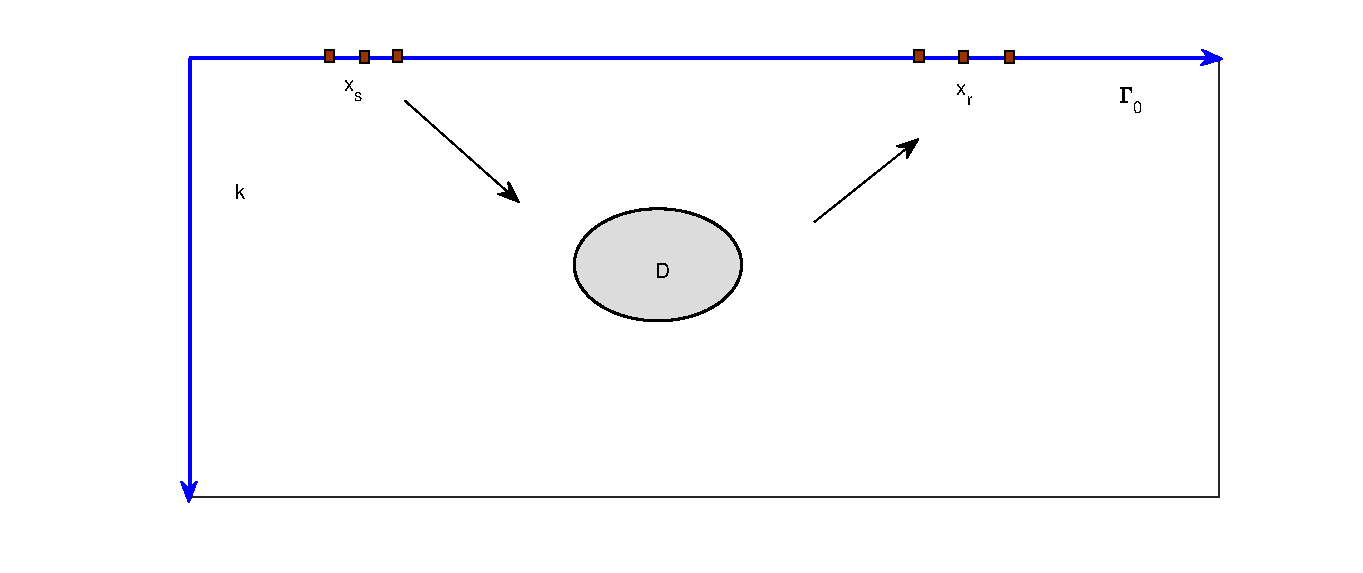
\includegraphics[width=\textwidth]{./Img/graphic/half_forward.eps}
	\caption{半空间弹性波障碍物散射模型} \label{figure_half}
\end{figure}
 令 $D\subset\R_+^2=\{(x_1,x_2)^T\in\R^2:x_2>0\}$ 是嵌入在半空间中的有界 Lipschitz 区域, 其中 $\nu$ 是边界 $\Ga_D$ 的单位外法向。 我们假设入射波是由位于半空间表面 $\Ga_0=\{(x_1,x_2)^T\in\R^2:x_2=0\}$ 上的 $x_s$ 的点源激发,且其激发的极化方向为 $q\in\R^2$。 假设半空间中的背景介质是弹性介质,且其表面满足自由边界条件 (Traction Free), 于是入射波即为半空间弹性波的 Neumann Green 函数 $\N(x,x_s)$ 。
假设接收点 $x_r\in \Ga_0$, 于是接受到的测量数据为 $u_q(x_r,x_s)=u^s_q(x_r,x_s)+\N(x_r,x_s)q, x_r\in\Ga_0$, 其中 $u_q^s(x,x_s)$ 是如下半空间弹性波方程的散射解。
\be
& &\Delta_e u_q^s(x,x_s)+ \rho\,\omega^2u_q^s(x,x_s)= 0 \ \ \ \ \mbox{in }\R_+^2\bks \bar{D},\label{p1}\\
& &u^s_q(x,x_s)=-\N(x,x_s)q \ \ \mbox{on} \ \Ga_D,\\
& & \sigma(u_q^s(x,x_s))e_2=0 \ \ \mbox{on} \ \Ga_0,\label{p2}
\ee
这里 
$e_i$ 是沿着 $x_i$, $i=1,2$ 轴的单位向量。

如何通过测量到的散射数据来确定散射体 $D$ 的位置、大小和形状就是本章将
要解决的问题。
\section{点扩散函数}
在这一节中, 我们将详细介绍半空间弹性波点扩散函数(point spread function)。 点扩散函数是一种针对半空间介质中点源的成像函数。 在文献 \cite{RTMhalf_aco} 中, Chen 等提出了半空间声波的点扩散函数, 我们这里将其推广到半空间弹性波的情形, 特别的, 此时的点扩散函数是一个 $2\times2$ 的矩阵。
假设在半空间的表面 $\Ga_0^d=\{(x_1,x_2)^T\in\Ga_0: x_1\in (-d,d)\}$ 上接受到的数据为 Neumann Green 函数 $\N(x,y)$, 即位于 $y$ 处的点源的数据, 这里 $d>0$ 称为孔径。 于是, 我们将有限孔径点扩散函数 $\J_d(x,y)$, $x,y\in\R^2_+$ 定义为将数据 $\N(x,y)\chi_{(-d,d)}$ 作为在 $\Ga_0$ 上的 Dirichlet 边界条件的反传波长, 这里 $\chi_{(-d,d)}$ 为区间 $\chi_{(-d,d)}$ 上的特征函数。 
更准确的来说, $\J_d(x,y)e_j, j=1,2,$ 是如下散射问题的解:
\ben
& &\De_e[\J_d(x,y)e_j]+\om^2[\J_d(x,y)e_j]=0\ \ \mbox{in }\R^2_+,\\
& &\J_d(x,y)e_j=[\overline{\N(x,y)}e_j]\chi_{(-d,d)}\ \ \mbox{on }\Ga_0.
\een
利用弹性波的积分表示公式, 我们有,对于任意 $z,y\in\R^2_+$ ,
\ben
[\J_d(z,y)]_{ij}&=&e_i\cdot[\J_d(z,y)e_j]\\
&=&\int_{\Ga_0^d}\T_D(x,z)e_i\cdot\overline{\N(x,y)}e_jds(x),\ \ i,j=1,2,
\een
利用矩阵表达, 可以简化为
\be\label{jd}
\J_d(z,y)=\int_{\Ga_0^d}\T_D(x,z)^T\overline{\N(x,y)}ds(x).
\ee

观察表达式 (\ref{jd}) 及定理\ref{es_NGT}, 定理 \ref{es_DGT}不难发现, 当 $d\to\infty$时, $\J_d(z,y)$ 收敛。 因此, 自然地, 我们就可以定义半空间弹性波点扩散函数 $\J(x,y)\in \C^{2\times 2}$, $x,y\in\R^2_+$, 即为
\be\label{j}
\J(z,y)=\int_{\Ga_0}\T_D(x,z)^T\overline{\N(x,y)}ds(x).
\ee
于是, 利用极限吸收原理, 我们有
\ben
\J(z,y)=\lim_{\ep\to 0^+}\int_{\Ga_0} \T_D^{\,\omega(1+\i\ep)}(x,z)^T\,
\overline{\N_{\om(1+\i\ep)}(x,y)}ds(x),
\een
这里 $\T_D^{\,\omega(1+\i\ep)}(x,z)q=\sigma(\D_{\om(1+\i\omega)}(x,z)q)e_2,\forall q\in\R^2$。
利用 Parserval 等式, Lemma \ref{cauchy_pv}, (\ref{d2}) and (\ref{d1}), 我们可以得到
\be
\J(z,y)&=&\frac{1}{2\pi}\sum_{\al,\beta=p,s}{\rm p.v.}\int_{\R}\frac{{\Ta}(\xi)^T \overline{\Nb(\xi)}}{\overline{\delta(\xi)}} e^{\i (\mu_\alpha z_2-\overline{\mu}_\beta y_2)+\i(y_1-z_1)\xi} d\xi \nn \\
& &-\frac\i 2\sum_{\al,\beta=p,s}\left[\frac{{\Ta}(\xi)^T \overline{\Nb(\xi)}}{\overline{\delta'(\xi)}} e^{\i (\mu_\alpha z_2-\overline{\mu}_\beta y_2)+\i(y_1-z_1)\xi}\right]^{k_R}_{-k_R}. \label{d3}
\ee
为了后文讨论方便, 我们把 $\J(z,y)$ 中的一部分定义为:
\be
\F(z,y)&=&\frac{1}{2\pi}\int^{k_p}_{-k_p} \  \frac{{\Tp}(\xi)^T \overline{\Np(\xi)}}{\overline{\delta(\xi)}} e^{\i \mu_p (z_2- y_2)+\i(y_1-z_1)\xi} d\xi\nn \\
&&+\frac{1}{2\pi}\int^{k_s}_{-k_s} \  \frac{{\Ts}(\xi)^T \overline{\Ns(\xi)}}{\overline{\delta(\xi)}} e^{\i \mu_s (z_2- y_2)+\i(y_1-z_1)\xi} d\xi. \label{d4}
\ee

在研究半空间弹性波点扩散函数之前, 我们先来定义成像函数的采样区域。 令 $\Omega$ 为成像函数的采样区域, 定义 $h=\dist(\Omega,\Gamma_0)$ 是 $\Omega$ 与 $\Gamma_0$ 的距离。 我们假设存在常数 $0<c_1<1,c_2>0$ 成立
\be\label{d0}
|x_1|\leq c_1 d , \ \ \ \ \ \ \ \ |x-y|\leq c_2 h ,\ \ \ \ \forall x,y \in \Omega.
\ee
\begin{remark}
	上述假设中, 第一个条件代表成像函数的采样区域不能太靠近孔径边缘, 第二个条件代表采样区域的尺寸相比于其与 $\Ga_0$的距离不能太大。第二个条件通常是合理的, 因为我们感兴趣的障碍物的尺寸大小要比入射波的波长小或是相当, 也就是 $k_s h\gg 1$。
\end{remark}

下面的引理不仅说明了 $\J(z,y)$ 是 $\J_d(z,y)$ 在 $d\to\infty$ 的极限, 而且还给出了 $\J_d(z,y)$ 与 $\J(z,y)$ 关于 $(h/d)$ 的误差估计。
\begin{lem} \label{error_jd}
	假设 $k_s h\geq 1$ 和 $d\gg h$ 。 对于任意 $z,y\in\Omega$ , 我们有
	\ben
	& &|\J(z,y)-\J_d(z,y)|+k_s^{-1}|\nabla_y(\J(z,y)-\J_d(z,y))| \\
	&\leq&\frac{C}{\mu} \left[\left(\frac{h}{d}\right)^{2}+(k_s h)^{1/2}e^{-k_s h\sqrt{\kappa_R^2-1}}\left(\frac{h}{d}\right)^{1/2}\right],
	\een
	这里常数 $C$ 只依赖于 $\kappa$ 。
\end{lem}
\debproof
我们利用定理 \ref{es_NGT} 和定理 \ref{es_DGT},作变量替换 $ t=x_1-z_1$,得到当 $k_s h\geq 1$ 和 $d\gg h$ 时有
\ben
& &\left| \int_{d}^{\infty} \left[\T_D(x,z)^T\overline{\N(x,y)}\right]_{x_2=0}dx_1
\right| \\
&\leq&
\frac{C}{\mu}\int_{d}^{\infty}\frac{k_s^{1/2} z_2}{|x-z|^{3/2}}\left(
\frac{k_s^{-1/2} y_2}{|x-y|^{3/2}}+e^{-\sqrt{k_R^2-k_s^2}y_2}\right) dx_1\\
&\leq&
\frac{C}{\mu}\int_{(1-c_1)d/h}^{\infty}\left(\frac{1}{(1+t^2)^{3/2}}+\frac{(k_s h)^{1/2}}{(1+t^2)^{3/4}} e^{-\sqrt{k_R^2-k_s^2}h}\right)  dt\\
&\leq&\frac{C}{\mu} \left[\left(\frac{h}{d}\right)^{2}+\frac{(k_s h)^{1/2}}{ e^{\sqrt{k_R^2-k_s^2}h}}\left(\frac{h}{d}\right)^{1/2}\right].
\een
上面的第二不等式我们使用了 (\ref{d0}) 的假定。 类似地, 我们也可以证明在 $(-\infty,-d)$ 上的不等式估计。 这就说明了 $\J(z,y)-\J_d(z,y)$ 的误差大小。 同样地, 针对 $\nabla_y(\J(z,y)-\J_d(z,y))$ 的估计也可以被证明。
\finproof

 有了以上引理, 现在我们可以只研究 $\J(z,y)$ 的性质, 然后通过引理 \ref{error_jd} 得到 $\J_d(z,y)$ 的性质。 由于我们只关心障碍物远离边界 $\Ga_0$ 时的情况, 即 $k_s h \gg 1$ , 所以, 针对点扩散函数 $\J(z,y)$, 我们希望将其分成两项, 其中第一项与 $k_s h$ 无关, 即主项; 第二项关于 $k_s h $ 是衰减的。
下面, 我们将说明当 $z,y\in\Om$时, $\F(z,y)$ 是 $\J_d(z,y)$ 的 $\F(z,y)$ 主项, 而且当 $|z-y|\to\infty$ 时, 它是衰减的。 特别地, 对于 $\F(z,y)$ 的虚部 $|\Im\F_{ii}(z,y)|, i=1,2$, 其在 $z=y$ 处存在峰值。

下面我们将用几个引理来说明 $\J_d(z,y)-\F(z,y)$ 关于 $k_s h$ 及 $h/d$ 的误差估计。 如下引理将说明式 (\ref{d3}) 中的第二项是随着 $k_s h$ 变大而指数衰减的。 

\begin{lem}\label{decay_1}
	存在只与 $\kappa$ 有关的常数 $C$, 当 $z,y\in\Om$ 时, 成立
	\ben
	\left|\sum_{\al,\beta=p,s}\left[\frac{{\Ta}(\xi)^T \overline{\Nb(\xi)}}{\overline{\delta'(\xi)}} e^{\i (\mu_\alpha z_2-\overline{\mu}_\beta y_2)+\i(y_1-z_1)\xi}\right]^{k_R}_{-k_R}\right|\le \frac C\mu e^{-\sqrt{k_R^2-k_s^2}h}.
	\een
\end{lem}
\debproof
观察式子 (\ref{d1}) , (\ref{d2}) ,我们发现, 对于 $\al=p,s$, 成立 $|\Ta(\pm k_R)|\le Ck_R^2/k_s^2\le C$, $|\Na(\pm k_R)|\le Ck_R^3$ 。利用引理 \ref{delta}, 该引理得证。
\finproof

\begin{lem}\label{lem:3.3}
	假设 $g(t)\in C^1(\R)\cap L^1(\R)$ 。存在只与 $\kappa$ 有关的常数 $C$,对于任意 $z,y\in\Om$ 成立
	\ben
	& & \left|{\rm p.v.}\int_{|\xi|>k_s}\frac{g(\xi)}{\delta(\xi)}d\xi\right| \\
	&\leq& Ck_s^{-4}\int_{|\xi|>k_s}|g(\xi)|d\xi+
	Ck_s^{-3}\max_{\xi\in(k_R-d_R,k_R+d_R)}(|g(\xi)|+k_s|g'(\xi)|).
	\een
	这里 $d_R =(k_R-k_s)/2$。
\end{lem}
\debproof
不失一般性,这里我们只针对在区间 $(k_s,\infty)$ 上的积分来证明该引理。 如引理 Lemma \ref{delta} 中一样, 我们有如下表示 $\de(\xi)=(\xi^2-k_R^2)\de_1(\xi)$ , 其中当 $\xi>k_s$ 时, $\de_1(\xi)\not=0$ 。 利用 Cauchy 主值的定义, 我们有
\be\label{l4}
\pv\int^\infty_{k_s}\frac{g(\xi)}{\delta(\xi)}d\xi&=&\int_{k_s}^{k_R-d_R}\frac{g(\xi)}{\delta(\xi)}d\xi+
\int^\infty_{k_R+d_R}\frac{g(\xi)}{\delta(\xi)}d\xi\nn\\
& &+\int^{k_R+d_R}_{k_R-d_R}\frac{g(\xi)((\xi+k_R)\de_1(\xi))^{-1}-g(k_R)(2k_R\de_1(k_R))^{-1}}{(\xi-k_R)}d\xi.
\ee
利用引理 \ref{delta}, 我们易得
\ben
\left|\int_{k_s}^{k_R-d_R}\frac{g(\xi)}{\delta(\xi)}d\xi+
\int^\infty_{k_R+d_R}\frac{g(\xi)}{\delta(\xi)}d\xi\right|\le Ck_s^{-4}\int^\infty_{k_s}|g(\xi)|d\xi.
\een
同样利用引理 \ref{delta} 中对 $\de(\xi),\de_1(\xi)$ 的估计及中值定理,我们可以得到
\ben
& &|\int^{k_R+d_R}_{k_R-d_R}\frac{g(\xi)((\xi+k_R)\de_1(\xi))^{-1}-g(k_R)(2k_R\de_1(k_R))^{-1}}{(\xi-k_R)}d\xi| \\
&\leq& 2d_R\max_{\xi\in(k_R-d_R,k_R+d_R)}(|\frac{g'(\xi)}{(\xi+k_R)\de_1(\xi)}|
\\
& &+|\frac{g(\xi)\delta_1(\xi)}{(\xi+k_R)\de_1(\xi))^2})|+|\frac{g(\xi)\delta_1'(\xi)}{(\xi+k_R)\de_1(\xi))^2}|)\\
&\leq&Ck_s^{-3}\max_{\xi\in(k_R-d_R,k_R+d_R)}(|g(\xi)|+k_s|g'(\xi)|)
\een
引理得证。
\finproof

下面的引理继续说明了 $\J(z,y)$ 中在区间 $|\xi|>k_s$ 上相应的积分是随 $k_s h$ 增大衰减的。
\begin{lem}\label{decay_2}
	令 $k_sh\ge 1$。 存在只与 $\kappa$ 有关的常数$C$, 对任意  $z,y\in\Om$ 成立
	\ben
	\left|\sum_{\al,\beta=p,s}{\rm p.v.}\int_{|\xi|>k_s}\frac{{\Ta}(\xi)^T \overline{\Nb(\xi)}}{\overline{\delta(\xi)}} e^{\i (\mu_\alpha z_2-\overline{\mu}_\beta y_2)+\i(y_1-z_1)\xi} d\xi\right|\le \frac C\mu(k_sh)^{-1}.
	\een
\end{lem}
\debproof
关于 $\al,\beta=p,s$, 我们定义 $g_{\al\beta}(\xi)=\Ta(\xi)^T\overline{\Nb(\xi)}e^{\i (\mu_\alpha z_2-\overline{\mu}_\beta y_2)+\i(y_1-z_1)\xi}$。于是利用引理 \ref{lem:3.3},我们可以易得
\ben
& &\left|\pv\int_{|\xi|>k_s}\frac{g_{\al\beta}(\xi)}{\overline{\de(\xi)}}d\xi\right| \\
&\le&\frac {C}{k_s^6\mu}\int^\infty_{k_s}|\xi|^5e^{-\sqrt{\xi^2-k_s^2}(y_2+z_2)}d\xi+\frac C\mu(k_sh) e^{-\sqrt{(k_R-d_R)^2-k_s^2}(y_2+z_2)}\\
&\le&\frac C\mu\int^\infty_1t^5e^{-\sqrt{t^2-1}k_s(y_2+z_2)}dt+\frac C\mu (k_sh) e^{-\sqrt{(k_R-d_R)^2-k_s^2}(y_2+z_2)}\\
&\le&\frac C\mu (k_sh)^{-1}+\frac C\mu (k_sh) e^{-\sqrt{(k_R-d_R)^2-k_s^2}(y_2+z_2)},
\een
这里我们使用了条件 $y_2,z_2 \geq h$ 和 $d_R=(k_R-k_s)/2\ge C_1k_s$, 其中常数 $C_1>0$ 只依赖于 $\kappa$。
又因为上面不等式的第二项是关于 $k_sh$ 指数衰减,则可以被 $(k_s h)^{-1}$ 控制。 引理得证。
\finproof
下面的引理将有助于我们分析在区间 $(-k_p,k_p)$ 上 , 当 $\al\neq\beta$时的积分。
\begin{lem}\label{cross_term}
	令 $\phi(t)=\sqrt{1-t^2}-\tau\sqrt{\kappa^2-t^2}+\nu t$, 这里 $\kappa\in (0,1), \tau\ge\tau_0>0, \nu\in\R$。
	存在仅依赖于 $\kappa, \tau_0$ 而与 $\nu$ 无关的常数 $C$ , 对于任意 $\lam\ge 1$ 以及 $f\in C[0,\kappa]$ 且其存在绝对连续的导函数, 成立:
	\ben
	& &
	\left|\int^\kappa_{-\kappa}f(t)e^{\i\lam\phi(t)}dt\right|+\left|\int^\kappa_{-\kappa}f(t)e^{-\i\lam\phi(t)}dt\right| \\
	&\leq& C\lambda^{-1/4}\left(|f(0)|+\int_{-\kappa}^{\kappa}|f'(t)|dt\right).
	\een
\end{lem}
\debproof
这里我们只要证明第一个在区间 $(0,\kappa)$ 上的积分的估计。 在区间 $(-\kappa,0)$ 上的积分的估计可以被类似证明,我们省略其证明细节。 通过简单的求导计算, 我们可以得到对于任意 $t\in (0,\kappa), m\ge 2$, 函数 $\phi(t)$ 的 $m$次导函数为 $\phi^{(m)}(t)=\tau\kappa^{-(m-1)}\psi_m(t/\kappa)-\psi_m(t)$, 其中
\ben
& &\psi_2(t)=(1-t^2)^{-3/2},\ \ \psi_3(t)=3t(1-t^2)^{-5/2},\ \  \\
& &\psi_4(t)=3(1+4t^2)(1-t^2)^{-7/2}.
\een
显然有, $\psi_m(t),m\ge 2$ 在区间 $(0,\kappa)$ 中是单调增函数。 

首先我们考虑当 $\tau\ge \kappa^2$ 时的情况。 这就意味着 $\tau\kappa^{-3}\ge\kappa^{-1}$ 而且有
\ben
\phi^{(4)}(t)\ge(\kappa^{-1}-1)\psi_4(t)\ge 3(\kappa^{-1}-1).
\een
利用 Van der Corput 引理 \ref{van},立即得到
\be\label{k2}
\left|\int^\kappa_{0}f(t)e^{\i\lam\phi(t)}dt\right|\leq C\lambda^{-1/4}\left(|f(0)|+\int_{-\kappa}^{\kappa}|f'(t)|dt\right).
\ee

接下去,我们考虑当 $\tau<\kappa^2$ 时的情况。 令 $\phi''(t)=0$, 可以得到
\ben
\tau\kappa^{-1}(1-(t/\kappa)^2)^{-3/2}=(1-t^2)^{-3/2}
\een 
易得 $\phi''(t)$ 在区间 $(0,\kappa)$ 上存在且只存在一个零点 $t=t_2$, 且有
\ben
t_2^2=\kappa^2-\frac{1-\kappa^2}{(\tau\kappa^2)^{-2/3}-1},
\een
观察 $\phi'''(t)$ , 我们可以得到, 当 $\kappa^3\le\tau<\kappa^2$ 时,在 $(0,\kappa)$ 上成立 $\phi'''(t)\ge 0$ ; 或是当 $\tau<\kappa^3$ 时, 有 $\phi'''(t)$ 在区间 $(0,\kappa)$ 上有且仅有一个零点 $t_3$, 且有
\ben
 t_3^2=\kappa^2-\frac{1-\kappa^2}{(\tau\kappa^2)^{-2/5}-1}.
\een
于是当 $\kappa^3\le\tau<\kappa^2$ 时, $\phi''(t)$在区间 $(0,\kappa)$ 为式单调增函数。 因此对于充分小的 $\de>0$,
\be\label{k3}
\hskip-1cm|\phi''(t)|\ge \min(|\phi''(t_2+\de)|,|\phi''(t_2-\de)|),\ \ \forall t\in (0,t_2-\de)\cup( t_2+\de,\kappa).
\ee
另一方面, 当$\tau<\kappa^3$ 时, 可以得到 $t_3<t_2$。而且成立当 $t\ge t_3$ 时有 $\phi'''(t)\ge 0$ 以及当 $t\le t_3$ 时有 $\phi'''(t)\le 0$ 。因此 $\phi''(t)$ 在区间 $(t_3,\kappa)$ 上单调递增而在 $(0, t_3)$ 上单调递减。 于是
\be\label{k4}
|\phi''(t)|\ge \min(|\phi''(t_2+\de)|,|\phi''(t_2-\de)|,|\phi''(0)|),\ \ \forall t\in (0,t_2-\de)\cup(t_2+\de,\kappa).
\ee

为了估计 $|\phi''(t_2\pm\de)|$ 的正下界, 我们观察到 $\tau\kappa^2<\kappa^4$。 因此, 我们得到 
\ben
t_2^2\ge\kappa^2-(1-\kappa^2)/(\kappa^{-8/3}-1).
\een
于是即得 $|\phi'''(t_2)|\ge c_0\tau\ge c_0\tau_0$ 其中常数 $c_0$ 仅依赖于 $\kappa$。
此外,对于任意 $t\in [t_2-\de,t_2+\de]$,有
\ben
|\phi'''(t)-\phi'''(t_2)|\le\max_{t\in [t_2-\de,t_2+\de]} |\phi''''(t)||t-t_2|\le c_1\de
\een
其中常数 $c_1$ 仅依赖于 $\kappa$。于是,如果取 $\de\le c_0\tau_0/(2C_1)$,对于$t\in[t_2-\de,t_2+\de]$, 就有 $|\phi'''(t)|\ge c_0\tau_0/2$。 

利用中值定理,我们可以得到 $|\phi''(t_2\pm\de)|\ge (c_0\tau_0/2)\de$。 观察到 $|\phi''(0)|=1-\tau\kappa^{-1}\ge 1-\kappa$, 从估计式 (\ref{k3})-(\ref{k4}) 我们可以得到对于充分小的 $\de>0$,
\be\label{k5}
|\phi''(t)|\ge (c_0\tau_0/2)\de,\ \ \forall t\in (0,t_2-\de)\cup( t_2+\de,\kappa).
\ee
现在,我们可以将积分分解成如下
\ben
& &\int^{\kappa}_0f(t)e^{\i\lam\phi(t)}dt\\
&=&\int^{t_2-\de}_0f(t)e^{\i\lam\phi(t)}dt+\int^{t_2+\de}_{t_2-\de}f(t)e^{\i\lam\phi(t)}dt+\int_{t_2+\de}^\kappa f(t)e^{\i\lam\phi(t)}dt\\
&:=&{\rm II}_1+{\rm II}_2+{\rm II}_3.
\een
利用不等式 (\ref{k5}) 及 Van der Corput 引理 \ref{van}, 我们有
\ben
|{\rm II}_1+{\rm II}_3| \le C(\lam\de)^{-1/2}\left(|f(0)|+\int^\kappa_0|f'(t)|dt\right).
\een
显然有 $|{\rm II}_2|\le 2\de\max_{t\in (0,\kappa)}|f(t)|$。我们取 $\de=\lam^{-1/3}$, 就可以得到
\ben
\left|\int^\kappa_{0}f(t)e^{\i\lam\phi(t)}dt\right|\leq C\lam^{-1/3}\left(|f(0)|+\int_{-\kappa}^{\kappa}|f'(t)|dt\right).
\een
联合 (\ref{k2}), 引理得证。
\finproof

下面的定理是本节的重要定理, 他说明了点扩散函数 $\J(z,y)$ 与其主项 $\F(z,y)$ 之间关于 $k_s h$ 的误差控制。
\begin{thm}\label{J_F_diff}
	令 $k_s h\ge 1$ 。存在只与 $\kappa$ 有关的常数 $C$, 对于任意 $z,y\in\Om$, 成立
	\ben
	|\J(z,y)-\F(z,y)|+k_s^{-1}|\na_y(\J(z,y)-\F(z,y))|\leq \frac{C}{\mu}(k_s h)^{-1/4}.
	\een
\end{thm}

\debproof
通过利用引理 \ref{decay_1}及引理 \ref{decay_2}, 观察 $\J(z,y),\F(z,y)$ 的定义 (\ref{d3})-(\ref{d4}), 我们只需要估计如下两项
\ben
& &\frac 1{2\pi}\sum_{\al,\beta=p,s}\int_{-k_s}^{k_s}\frac{{\Ta}(\xi)^T \overline{\Nb(\xi)}}{\overline{\delta(\xi)}} e^{\i (\mu_\alpha z_2-\overline{\mu}_\beta y_2)+\i(y_1-z_1)\xi} d\xi-\F(z,y)\\
\hskip-1cm&=&\frac {1}{2\pi}\sum_{\stackrel{\al,\beta=p,s}{_{(\al,\beta)\not= (s,s)}}}\int_{(-k_s,k_s)\backslash[-k_p,k_p]}\frac{{\Ta}(\xi)^T \overline{\Nb(\xi)}}{\overline{\delta(\xi)}} e^{\i (\mu_\alpha z_2-\overline{\mu}_\beta y_2)+\i(y_1-z_1)\xi} d\xi\\
\hskip-1cm&+&\frac 1{2\pi}\int_{-k_p}^{k_p}\left[\frac{\Tp(\xi)\overline{\Ns(\xi)}}{\overline{\de(\xi)}}e^{\i(\mu_py_2-\mu_s z_2)}+\frac{\Ts(\xi)\overline{\Np(\xi)}}{\overline{\de(\xi)}}e^{\i(\mu_sy_2-\mu_p z_2)}\right]e^{\i(y_1-z_1)\xi}d\xi\\
\hskip-1cm&:=&{\rm II}_1+{\rm II}_2.
\een
当 $k_p<|\xi|<k_s$ 时, 由引理 \ref{delta} 得, 我们知道有 $|\de(\xi)|\ge Ck_s^4$ 。 于是, 对于 $\al,\beta=p,s$, 我们有 $|\Ta(\xi)|\le C, |\Nb(\xi)|\le C\mu^{-1}k_s^2$。 于是, 我们马上可以得到如下不等式:
\ben
|{\rm II_1}|\le \frac{C}{k_s\mu}\int^{k_s}_{k_p}e^{-\sqrt{\xi^2-k_p^2}h}d\xi\le\frac C\mu (k_sh)^{-1}.
\een
而对于式子 ${\rm II}_2$ 我们将会使用引理 \ref{cross_term}。 通过简单的变量替换 $\xi=k_s t$, 我们可以把式 ${\rm II}_2$ 中的第一项转化成引理 \ref{cross_term} 中的形式, 即有
\ben
f(t)=k_s\frac{\Tp(k_st)\overline{\Ns(k_st)}}{\overline{\de(k_st)}},\ \ \ \lam=k_sz_2,\tau=\frac{y_2}{z_2},\nu=\frac{y_1-z_1}{z_2}.
\een
利用前面针对采样区域的尺寸的假设 (\ref{d0}), 直接利用引理 \ref{cross_term} 就可以得到,
\ben
\left|\int_{-k_p}^{k_p}\frac{\Tp(\xi)\overline{\Ns(\xi)}}{\overline{\de(\xi)}}e^{\i(\mu_py_2-\mu_s z_2)}d\xi\right|\le\frac{C}{\mu}(k_sh)^{-1/4}.
\een
而式子 ${\rm II}_2$ 中的第二项也可以被类似估计。 且 $|\na_y(\J(z,y)-\F(z,y))|$ 的估计也可以被类似证明, 这里不再赘述。 引理得证。
\finproof
\begin{figure}[htbp]
	\centering
	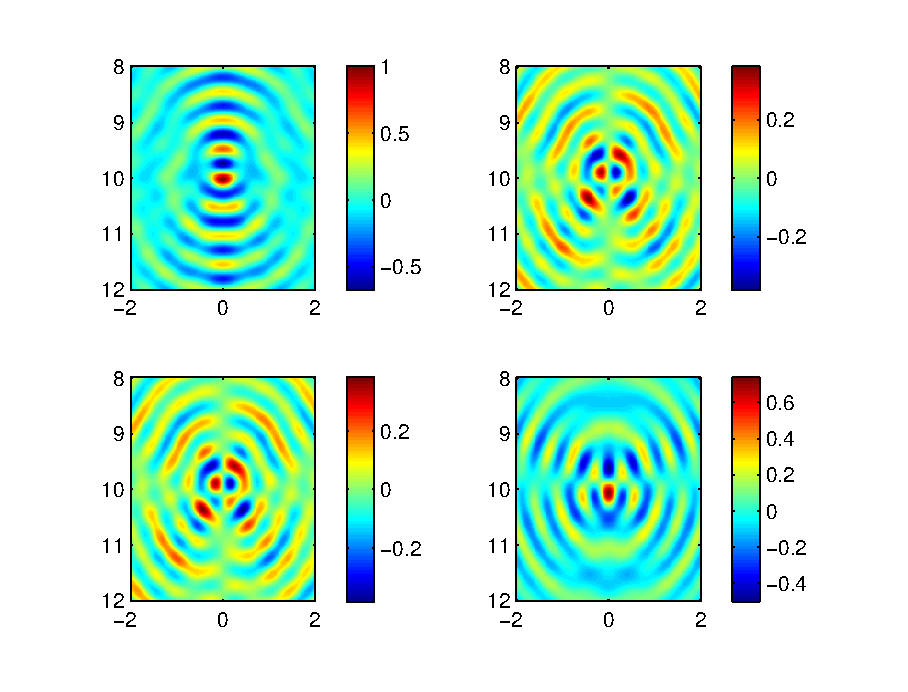
\includegraphics[width=\textwidth]{./Img/graphic/psf_om_2_lm_5_mu_25_im.eps}	
	\caption{$-Im(J_d(z,y))$ for $y=(0,8)^T$, $\omega=2\pi$, $d=100$}\label{figure_green}
\end{figure}
\begin{figure}[htbp]
	\centering
	\includegraphics[width=\textwidth]{./Img/graphic/green_om_2_lm_5_mu_25_im.eps}	
	\caption{$Im(G(z,y))$ for $y=(0,8)^T$, $\omega=2\pi$}\label{figure_psf}
\end{figure}

下面的引理告诉我们,点扩散函数 $\F(z,y)$ 的虚部与弹性波基本解 $\Im\G(z,y)$ 的虚部有相似的函数特性。于是, 利用定理 \ref{J_F_diff} 和引理 \ref{error_jd}, 当 $d\gg h$ 和 $k_s h\gg 1$, 我们可以认为 $\J_d(z,y)$ 的虚部也与弹性波基本解 $\Im\G(z,y)$ 的虚部有相似的函数特性, 见图 \ref{figure_psf} 和 图\ref{figure_green} 所展示。

\begin{remark}
	如图\ref{figure_psf} 和 图\ref{figure_green}中, 每幅图中4副子图, 其中子图的位置对应相应矩阵该位置的函数。其中, 每幅图的采样区域都为 $[-2,2]\times[8,12]$, 角频率 $\om=2\pi$, {Lam\'{e}} 常数 $\lambda=0.5$, $\mu=0.25$。 特别地, 每幅子图中, 颜色越深代表该处的值越大, 因此我们可以看到图\ref{figure_psf} 和 图\ref{figure_green}中对角线上的子图, 他们颜色的最深处正式图的中心位置, 即代表峰值在 $z=y$ 处。
\end{remark}
\begin{thm} \label{thm:3.2}
	对于任意 $z,y\in \R_+^2$, $\F(z,y)^T=\F(z,y)$。 当 $z=y$ 时,  $\Im [\F(z,y)]_{12} = \Im [\F(z,y)]_{21} =0$ 以及
	\be\label{d6}
	-\Im [\F(z,y)]_{ii}\geq \frac{1}{4(\lambda+2\mu)} \ , \ i =1 ,2.
	\ee
	当 $z\neq y$ 时,
	\be\label{d7}
	|\F(z,y)|&\le \frac{C}{\mu}\left(\frac 1{(k_s|z-y|)^{1/2}}+\frac 1{k_s|z-y|}\right),
	\ee
	这里的常数 $C$ 只依赖于 $\kappa$。
\end{thm}

\debproof
将式子 (\ref{d1}) 和式子 (\ref{d2}) 代入式子 (\ref{d4}), 我们可以得到
\be   
\F(z,y)&=&-\frac{1}{2\pi}\int_{-k_p}^{k_p} \frac{\i k_s^2\mu_s}{\mu\gamma(\xi)\delta(\xi)}
\Bigg(
\begin{array}{cc}
	\xi^2 & -\xi\mu_p \\
	-\xi\mu_p & \mu_p^2
\end{array}\Bigg)e^{\i\mu_p (z_2-y_2) +\i\xi(y_1-z_1)}d\xi \nn\\
\hskip-1.5cm& &-\frac{1}{2\pi}\int_{-k_p}^{k_p} \frac{\i k_s^2\mu_p}{\mu\gamma(\xi)\delta(\xi)}
\Bigg(
\begin{array}{cc}
	\mu_s^2 & \xi\mu_s \\
	\xi\mu_s & \xi^2
\end{array}		\Bigg)e^{\i\mu_s (z_2-y_2) +\i\xi(y_1-z_1)}d\xi \nn\\ 
\hskip-1.5cm& &
-\frac{1}{2\pi}\int_{(-k_s,k_s)\bks[-k_p,k_p]} \frac{\i(k_s^2-4\xi^2)\mu_p}{\mu\gamma(\xi)\overline{\delta(\xi)}}
\Bigg(
\begin{array}{cc}
	\mu_s^2 & \xi\mu_s \\
	\xi\mu_s & \xi^2
\end{array}		\Bigg)e^{\i\mu_s (z_2-y_2) +\i\xi(y_1-z_1)}d\xi \nn\\
\hskip-1.5cm&:=&{\rm III}_1+{\rm III}_2+{\rm III}_3. \label{d8}
\ee
由于 $\mu_p(\xi)$ 及 $\mu_s(\xi)$ 关于 $\xi$ 存在对称性, 所以我们易得当 $z=y$ 时, $\Im [\F(z,y)]_{12} = \Im [\F(z,y)]_{21} =0$。

现在我们来证明当 $i=j=1$ 时的不等式(\ref{d6}), 而其他情形时可以被类似证明, 这里将省略细节。 观察到, 当 $\xi\in (-k_p,k_p)$ 时,由引理 \ref{delta} 得 $\delta(\xi)\le k_s^4$ 及易得 $\mu_p\le\mu_s$。 于是当 $z=y$ 时:
\ben
& &-\Im ({\rm III}_1+{\rm III}_2)=\frac{1}{2\pi\mu}\int^{k_p}_{-k_p}\frac{k_s^2\mu_s}{\de(\xi)}d\xi\\
&\geq&\frac{1}{2\pi\mu}\int_{-k_p}^{k_p} \frac{\mu_p}{k_s^2}d\xi = \frac{1}{4(\lambda+2\mu)}.
\een
而当 $\xi\in(-k_s,k_s)\bks[-k_p,k_p]$时,成立 $\mu_p=\i\sqrt{\xi^2-k_p^2}$, 于是我们有
\ben
-{\rm III}_3=\frac{1}{2\pi\mu}\int_{(-k_s,k_s)\bks(-k_p,k_p)} \frac{-\mu_s^2\sqrt{\xi^2-k_p^2}(k_s^2-4\xi^2)}{(\xi^2+\i\mu_s\sqrt{\xi^2-k_p^2})(\varphi^2-\i4\xi^2\mu_s\sqrt{\xi^2-k_p^2})} d\xi.
\een
通过简单的直接计算, 我们有 \ben
\Im[(\xi^2+\i\mu_s\sqrt{\xi^2-k_p^2})(\varphi^2-\i4\xi^2\mu_s\sqrt{\xi^2-k_p^2})]=k_s^2\mu_s\sqrt{\xi^2-k_p^2}(k_s^2-4\xi^2).
\een
 通过分母有理化, 我们可以得到 $-\Im({\rm III}_3)\ge 0$。 因此, 当 $z=y$ 时, 我们有 $-\Im[\F(z,y)]_{11}\ge 1/[4(\lam+2\mu)]$ 。

当 $z\neq y$ 时, 我们可以有如下三角函数表示 $y-z=|y-z|(\cos\phi,\sin\phi)^T$ ,其中 $0\le\phi\le \pi$。 于是, 将此三角变量替换代入 ${\rm III}_1$, 我们可以得到
\ben
{\rm III}_1=\frac{1}{\mu}\int_{0}^{\pi} A(\theta,\kappa) e^{\i k_s |z-y| \cos(\theta-\phi)}d\theta,
\een
显然,简单的代入计算可以得到函数 $A(\theta,\kappa)$ 及其导函数 $\pa A(\theta,\kappa)/\pa\theta$ 在区间 $(0,\pi)$。 而且区间 $(0,\pi)$ 可以分割成若干个互补相交的子区间, 在每个子区间上成立 $|\cos(\theta-\phi)|\ge 1/\sqrt 2$ 或是 $|\sin(\theta-\phi)|\ge 1/\sqrt 2$ 以及 $-\sin(\theta-\phi)$ 在盖子区间上单调。 于是, 当$k_s|z-y|\ge 1$ 时,  Van der Corput 引理 \ref{van} , 我们易得
\ben
|{\rm III}_1|\le \frac C\mu\left(\frac 1{(k_s|z-y|)^{1/2}}+\frac 1{k_s|z-y|}\right).
\een
而当 $k_s|z-y|< 1$ 时,显然有 $|{\rm III}_1|\le C\mu^{-1}\le C\mu^{-1}(k_s|z-y|)^{-1}$。 而针对 ${\rm III}_2+{\rm III}_3$ 的估计可以类似地使用 Van der Corput 引理 \ref{van} 来证明。 引理得证。
\finproof

结合引理 \ref{error_jd}, 定理\ref{J_F_diff}, 定理\ref{thm:3.2} 及图\ref{figure_psf}, 我们发现点扩散函数 $J_d(z,y)$ 确实可以把位于 $y$ 的点源分辨出来, 即在 $z=y$ 处达到峰值, 在 $z$ 远离 $y$ 其值渐渐衰减。如文献 \cite{RTMhalf_aco} 中针对声波点扩散函数的表述, 我们也可以认为弹性波点扩展函数是对寻找弹性点源分辨率的度量函数。

为便于后文分析, 我们介绍如下在范数意义下的估计式。
\begin{lem}\label{lem:4.1}
	令 $k_s h\geq 1, d\gg h$, 存在只依赖于 $\kappa$ 却与 $k_s, h, d, d_D$ 无关的常数 $C$ , 对于任意 $z\in\Om$, $j=1,2$, 成立
	\ben
	& &\|\F(z,\cdot)e_j\|_{H^{1/2}(\Ga_D)}+\|\sigma(\F(z,\cdot)e_j)\nu\|_{H^{-1/2}(\Ga_D)}\le\frac C\mu(1+k_sd_D),\\
	& &\|\R_d(z,\cdot)e_j\|_{H^{1/2}(\Gamma_D)}+\|\sigma(\R_d(z,\cdot)e_j)\nu\|_{H^{-1/2}(\Gamma_D)} \le
	\frac{C}{\mu}(1+k_sd_D)\left[\left(\frac hd\right)^{2}+(k_sh)^{-1/4}\right],
	\een	
	其中 $\R_d(z,\cdot)=\J_d(z,\cdot)-\F(z,\cdot)$.
\end{lem}


\debproof
由 $\F(z,\cdot)$ 的定义 (\ref{d4}), 我们易得:
\ben
|F(z,y)|\leq \frac{C}{\mu}
\een 
于是, 上面第一估计式可有不等式 (\ref{q0}) 立即得到。 第二估计式可有不等式 (\ref{q0}), 由引理 \ref{error_jd} 和定理 \ref{J_F_diff} 立即得到。这里我们将不再赘述细节。 引理得证。
\finproof
\section{逆时偏移算法}
这一节, 我们将提出半空间弹性波散射问题的逆时偏移算法 (Reverse Time Migration, RTM)。 该逆时偏移算法是对文献 \cite{RTMhalf_aco} 中半空间声波散射问题的逆时偏移算法的一个推广。 我们的逆时偏移算法可以分成两步 \cite{zhang2009,Zhang2007}, 第一步为将在半空间表面的孔径 $\Ga_d$ 上接受到的 s-波与 p-波的混合全波数据取复共轭化, 然后反传到半空间中。 第二步,将反传后的数据和入射波数据在采样区域 $\Om$ 内进行互相关, 然后关于各个炮点进行叠加。特别地,类似与文献 \cite{RTMhalf_aco} , 这里的入射波是将点源放在 $\Ga_d$ 上, 然后作为 Dirichlet 边界条件后弹性波方程的解。而反传波是将接受到的数据共轭化后作为 Dirichlet 边界条件后弹性波方程的解。

\begin{alg}\label{alg_rtm}
	假设在 $\Ga_d$ 内均匀分布着 $N_s$ 个发射器, 位于 $x_s, \ s= 1,...,N_s$, 及分布着 $N_r$ 个接收器, 位于 $x_r, \ r=1,...,N_r$。 假设障碍物 $D\subset \Om$。 假设散射数据 $u_q^s(x_r,x_s)$ 为在 $x_r$ 处接受, 由位于 $x_s$ 处的点源沿着极化方向 $q=e_1, e_2$ 激发。
	
	$1^\circ$ 反传: 计算反传波 $v_q(x,x_s)$ 是如下半空间弹性波散射问题的解
	\ben
	& &\Delta_e v_q(x,x_s) + \omega^2 v_q(x,x_s) =0 \ \ \ \ \ \mbox{\rm in } \ \ \R^2_+, \\
	& &v_q(x,x_s)=\frac{|\Ga_0^d|}{N_r}\sum_{r=1}^{N_r}\overline{u_q^s(x_r,x_s)}\delta_{x_r}(x) \ \ \mbox{\rm on }  \ \ \Ga_d.
	\een
	
	$2^\circ$ 互相关: 对于任意 $q\in\R^2$,令入射波 $u^i_q$ 为如下半空间弹性波方程的解
	\ben
	& &\Delta_e u_q^i(x,x_s) + \omega^2 u_q^i(x,x_s) =0 \ \ \mbox{\rm in } \ \ \R^2_+,\ \ \\ & &u^i_q(x,x_s)=q\de_{x_s}(x)\ \ \mbox{on } \ \ \Ga_d.
	\een
	
	对于任意 $z\in\Om$, 计算成像函数:
	\be\label{cor1} 
	I_d(z)=\Im\sum_{q=e_1,e_2}\left\{\frac{|\Gamma_0^d|}{N_s}\sum^{N_s}_{s=1} u^i_q(z,x_s)\cdot v_q(z,x_s)\right\}. 
	\ee
\end{alg}
于是, 由 Green 表示公式可以得到:
\ben
& &u^i_q(x,x_s)=\T_D(x_s,x)^Tq, \\
& &v_q(x,x_s)\cdot e_j=\frac{|\Ga_0^d|}{N_r}\sum_{r=1}^{N_r}\T_D(x_r,x)e_j\cdot\overline{u_q^s(x_r,x_s)},
\een 
于是马上可以得到:
\be\label{cor}
I_d(z)=\Im\sum_{q=e_1,e_2}\left\{\frac{|\Gamma_0^d|^2}{N_sN_r}\sum^{N_s}_{s=1}\sum^{N_r}_{r=1}
[\T_D(x_s,z)^Tq]\cdot[\T_D(x_r,z)^T\overline{u^s_q(x_r,x_s)}]\right\}.
\ee

上面的成像函数是离散形式的, 可以直接用于数值计算。 为了便于后面的理论分析, 我们令 $N_s,N_r\to\infty$, 于是离散形式的成像函数 (\ref{cor1}) 可以看成是采用数值积分对如下连续形式的成像函数的一种积分逼近:
\be
\hat{I}_d(z)=\Im\sum_{q=e_1,e_2}\int_{\Gamma_0^d}\int_{\Gamma_0^d}\,
[\T_D(x_s,z)^Tq]\cdot[\T_D(x_r,z)^T\overline{u^s_q(x_r,x_s)}]\,ds(x_r)ds(x_s).\label{cor2}
\ee


下面我们将障碍物的成像函数 $\hat I_d(z)$ 与前文中的点扩散函数 $\J_d(z,y)$ 联系起来。 有了前文中对 $\J_d(z,y)$ 相关分析结论,我们可以由此来分析半空间反弹性波散射问题的逆时偏移方法的分辨率。下面的定理, 告诉我们当采样点 $z$ 远离障碍物边界的时候, 成像函数在改点的值是非常小的。这种现象反映在后面的数值实验中, 就是在原理边界的时候, 在该处的颜色会非常浅。下面的定理是当障碍物边界为 Dirichlet 边界时的成像函数分辨率分析。 其它边界条件的相关结论可以被类似证明, 我们会不加证明地罗列在后文。
\begin{thm}\label{thm:4.3}
	对于任意 $z\in\Omega$, 令 $\U(z,x)\in\C^{2\times2}$ 且 $\U(z,x)e_j$, $j=1,2$, 是如下弹性波方程的散射解:
	\ben
	& &\Delta_e [\U(z,x)e_j]+ \omega^2[\U(z,x)e_j]= 0 \ \  \ \ x\in\R^2\bks \bar{D},  \\
	& &
	\U(z,x)e_j= -\overline{\F(z,x)}e_j \ \  \ \ x\in\Ga_D.  
	\een
	于是, 成像函数 $\hat{I}_d(z)$ 有如下表达:
	\be
	\hat{I}_d(z)=\Im\sum_{j=1}^2\int_{\Gamma_D}[\sigma(\U(z,x)e_j+\overline{\F(z,x)}e_j)\nu]\cdot [\overline{\F(z,x)}e_j]ds(x)+R_d(z),\label{id}
	\ee
	这里 
	\ben
	|R_d(z)|\leq C\mu^{-2}(1+\|T_1\|)(1+\|T_2\|)(1+k_s d_D)^3\left[\left(\frac hd\right)^{2}+(k_sh)^{-1/4}\right],
	\een
	其中常数 $C$ 仅依赖与 $\kappa$ 而与 $k_s,k_p, h, d, d_D$ 无关。
\end{thm}
\debproof
观察算法中的 (\ref{cor2}) 我们可以得到:
\be\label{g5}
\hat I_d(z)=\Im\sum_{q=e_1,e_2}\int_{\Ga_0^d}[\T_D(x_s,z)^Tq]\cdot\hat v_q(z,x_s)ds(x_s),
\ee
其中 $j=1,2$,
\ben
\hat v_q(z,x_s)\cdot e_j=\int_{\Ga_0^d}\T_D(x_r,z)e_j\cdot\overline{u^s_q(x_r,x_s)}ds(x_r).
\een
利用 (\ref{g2}) 我们得到 
\ben
u^s_q(x_r,x_s)\cdot e_i=\GG(u^s_q(\cdot,x_s),\N(\cdot,x_r)e_i), i=1,2,
\een
 于是有
\ben
\hat v_q(z,x_s)\cdot e_j&=&\int_{\Ga_0^d}\T_D(x_r,z)e_j\cdot\overline{[u^s_q(x_r,x_s)\cdot e_1,u^s_q(x_r,x_s)\cdot e_2]^T}ds(x_r)\\
&=&\GG(\overline{u^s_q(\cdot,x_s)},\left[\int_{\Ga_0^d}\sum^2_{i=1}[\T_D(x_r,z)]_{ij}\overline{\N(\cdot,x_r)}e_ids(x_r)\right]\,).
\een
利用 Neumann Green 函数的空间互易性 
\ben
\N(x,x_r)=\N(x_r,x)^T,
\een
 以及点扩展函数 $\J_d(\cdot,\cdot)$ 的定义 (\ref{jd}), 我们有
\be\nn
& &\int_{\Ga_0^d}\sum^2_{i=1}[\T_D(x_r,z)]_{ij}\overline{\N(x,x_r)}e_ids(x_r)\\ \nn
&=&\int_{\Ga_0^d}\sum^2_{i=1}[\T_D(x_r,z)]_{ij}\overline{\N(x_r,x))^Te_i}ds(x_r)\\ \nn
&=&\int_{\Ga_0^d}(\T_D(x_r,z)e_j)^T\overline{\N(x_r,x)^T)}ds(x_r) \\  \nn
&=&\J_d(z,x)^Te_j. v \label{g6}
\ee
进一步可以推出
 \ben
 \hat v_q(z,x_s)e_j=\GG(\overline{u^s_q(\cdot,x_s)},\J_d(z,\cdot)^Te_j).
 \een
  将上式代入 (\ref{g5}) 中, 我们可以得到
\be\nn
\hat I_d(z)&=&\Im\sum_{j=1}\sum_{q=e_1,e_2}\int_{\Ga_0^d}[\T_D(x_s,z)^Tq\cdot e_j][\hat v_q(z,x_s)\cdot e_j]ds(x_s)
\\  \nn
&=&\Im\sum_{j=1}^2\GG(\sum_{k=1}^2[\T_D(x_s,z)^Te_k\cdot e_j]\overline{u^s_{e_k}(x,x_s)},\J_d(z,\cdot)^Te_j)
\\ 
\label{g3}
&=&\Im\sum_{j=1}^2\GG(\W(z,\cdot)e_j,\J_d(z,\cdot)^Te_j),
\ee
这里 $\W(z,x)\in \C^{2\times 2}$ 是一个 $2\times2$ 的矩阵, 定义为
\ben
\W(z,x)e_j=\int_{\Ga_0^d}\sum^2_{k=1}[\T_D(x_s,z)]_{kj}\overline{u^s_{e_k}(x,x_s)}ds(x_s),\ \ j=1,2.
\een
注意到 $\overline{\W(z,x)}e_j$ 可以看成是 $u^s_{e_k}(x,x_s)$ 加权叠加, 于是它满足如下方程:
\be\label{g7}
& &\De_e[\overline{\W(z,x)}e_j]+\om^2[\overline{\W(z,x)}e_j]=0\ \ \mbox{in } \ \R^2_+\bks\bar D,\ \ \ \\
& & \sigma(\overline{\W(z,x)}e_j)e_2=0\ \ \mbox{on } \ \Ga_0.
\ee
由于在边界 $\Gamma_D$, $u^s_{e_k}(x,x_s)$ 满足 Dirichlet 边界条件,即 $u^s_{e_k}(x,x_s)=-\N(x,x_s)e_k$。 于是利用式 (\ref{g6}) 我们得到
\be\nn
& &\overline{\W(z,x)}e_j\\ \nn
&=&-\int_{\Ga_0^d}\sum^2_{k=1}[\overline{\T_D(x_s,z)}]_{kj}\N(x,x_s)e_kds(x_s) \\
&=&-\overline{\J_d(z,x)}^Te_j.\label{g8}
\ee
现在我们定义矩阵 $\W_d(z,x)\in \C^{2\times 2}$ , 其中向量  $\W_d(z,x)e_j$, $j=1,2$ , 是如下半空间弹性波方程的散射解:
\be
& & \Delta_e [\W_d(z,x)e_j]+ \omega^2 [\W_d(z,x)e_j]= 0 \ \ \ \ \mbox{in }\R^2_+\bks \bar{D},\label{g9}\\
& &\W_d(z,x)e_j= -\overline{\F(z,x)}e_j \ \ \mbox{on } \ \ \Ga_D,\ \ \ \  \\
& &\sigma(\W_d(z,x)e_j)e_2=0 \ \ \ \ \ \ \ \mbox{on }  \ \ \ \Ga_0 \label{g10}
\ee
利用 (\ref{g3}) 我们可以推出:
\be
\hat I_d(z)&=&\Im\sum^2_{j=1}\GG(\W(z,\cdot)e_j,J_d(z,\cdot)^Te_j-\F(z,\cdot)e_j)\nn\\
& &+\Im\sum^2_{j=1}\GG(\W(z,\cdot)e_j-\overline{\W_d(z,\cdot)}e_j,\F(z,\cdot)e_j)\nn\\
& &+\Im\sum^2_{j=1}\GG(\overline{\W_d(z,\cdot)}e_j-\overline{\U(z,\cdot)}e_j,\F(z,\cdot)e_j)\nn\\
& &+\Im\sum^2_{j=1}\GG(\overline{\U(z,\cdot)}e_j,\F(z,\cdot)e_j) \nn \\
&:=&{\rm VI}_1+{\rm VI}_2+{\rm VI}_3+{\rm VI}_4.\label{g11}
\ee
观察 $\F(z,y)$ 的定义 ($\ref{d4}$), 易得 $\F(z,y)^T=\F(z,y)$。 利用引理 \ref{lem:4.1}, 
\ben
& &\|\J_d(z,\cdot)e_j\|_{H^{1/2}(\Ga_D)}+\|\sigma(\J_d(z,\cdot)e_j)\nu\|_{H^{-1/2}(\Ga_D)}\\ &\le&
\|\F(z,\cdot)e_j\|_{H^{1/2}(\Ga_D)}+\|\sigma(\F(z,\cdot)e_j)\nu\|_{H^{-1/2}(\Ga_D)}\\
& &+\|\R_d(z,\cdot)e_j\|_{H^{1/2}(\Ga_D)}+\|\sigma(\R_d(z,\cdot)e_j)\nu\|_{H^{-1/2}(\Ga_D)}\\
&\le&\frac C\mu (1+k_sd_D).
\een
这就意味着,通过 (\ref{g7})-(\ref{g8}) 以及引理 \ref{lem:4.1}, 可以得到:
\ben
|{\rm VI}_1|&\le&\sum_{j=1}^2\Big(\|\W(z,\cdot)e_j\|_{H^{1/2}(\Ga_D)}\|\sigma(\J_d(z,\cdot)^Te_j-\F(z,\cdot)e_j)e_2\|_{H^{-1/2}(\Ga_D)}\\
& &+\|\sigma(\W(z,\cdot)e_j)e_2\|_{H^{-1/2}(\Ga_D)}\|\J_d(z,\cdot)^Te_j-\F(z,\cdot)e_j\|_{H^{1/2}(\Ga_D)}\Big)\\
&\le&\frac C{\mu^2}(1+\|T_1\|)(1+k_sd_D)^2\left[\left(\frac hd\right)^{2}+(k_sh)^{-1/4}\right].
\een
类似地, 通过 (\ref{g7})-(\ref{g8}) 和 (\ref{g9})-(\ref{g10}), 及引理 \ref{lem:4.1} , 可以得到:
\ben
|{\rm VI}_2|\le\frac C{\mu^2}(1+\|T_1\|)(1+k_sd_D)^2\left[\left(\frac hd\right)^{2}+(k_sh)^{-1/4}\right].
\een
对于第三项 ${\rm VI}_3$, 我们可以针对 $\W_d(z,x)$ 和 $\U(z,y)$, 使用定理 \ref{thm:4.2} 和引理 {\ref{lem:4.1}, 可以得到:
	\ben
	|{\rm VI}_3|\le\frac C{\mu^2}(1+\|T_1\|)(1+\|T_2\|)(1+k_sd_D)^3(k_sh)^{-1/2}.
	\een
	最后, 由定义有, 当$z\in\Ga_D$ 时 $\U(z,x)e_j=-\overline{\F(z,x)}e_j$  $\Ga_D$。 于是,可以推出
	\ben
	{\rm IV}_4&=&\Im\sum^2_{j=1}\int_{\Ga_D}(\overline{\U(z,x)}e_j\cdot\sigma(\F(z,x)e_j)\nu-\sigma(\overline{\U(z,x)}e_j)\nu\cdot\F(z,x)e_j)ds(x)\\
	\hskip-1.5cm&=&-\Im\sum^2_{j=1}\int_{\Ga_D}\sigma(\overline{\U(z,x)}e_j+\F(z,x)e_j)\nu\cdot\F(z,x)e_jds(x)\\
	\hskip-1.5cm&=&\Im\sum^2_{j=1}\int_{\Ga_D}\sigma(\U(z,x)e_j+\overline{\F(z,x)}e_j)\nu\cdot\overline{\F(z,x)}e_jds(x).
	\een
	综上所述, 利用式子 (\ref{g11}), 引理得证。
	\finproof


由于本文中关心的障碍物都为扩展障碍物(Extended Obstacles),即为 $k_s d_D\approx 1$。由于 $k_s=2\pi/\lambda_s$, 这里 $\lambda_s$ 为 s-波的波长, 于是意味着障碍物的尺寸与入射波的s-波的波长相当。然后,通过定理 \ref{thm:4.3}, 我可以看到, 当障碍物 $D$ 远离半空间表面 $\Ga_0$ 时, 即 $k_s h \gg 1$, 且孔径较大时,即 $d\gg h$, 我们可以认为 $\R_d(z)$ 是非常小的。于是, 我们在这种情况下可以把式 (\ref{id}) 右端第一项看作是该成像函数的 $\hat I_d(z)$ 的主项
\ben
\hat{I}_d(z)&\approx&\Im\sum_{j=1}^2\int_{\Gamma_D}[\sigma(\U(z,x)e_j+\overline{\F(z,x)}e_j)\nu]\cdot [\overline{\F(z,x)}e_j]ds(x) \\
&:=&\hat{I}_F(z)
\een 

观察 $\F(z,x)$ 的表达式 (\ref{d8}), 对于任意 $z\in\Om$,存在标量函数 $A_j(\xi), B_j(\xi)$, $j=1,2$,可以将 $\F(z,x)$ 表示成
\ben\nn
\F(z,x)e_j&=&\int_{-k_p}^{k_p}A_j(\xi)\left(\begin{array}{c}
	\hskip-6pt-\xi \hskip-6pt \\
	\hskip-6pt \mu_p \hskip-6pt
\end{array}\right)e^{\i(z-x)\cdot(-\xi,\mu_p)^T}d\xi\\ \nn
& &+\int_{-k_s}^{k_s}B_j(\xi)\left(\begin{array}{c}
	\hskip-6pt\mu_s \hskip-6pt\\
	\hskip-6pt\xi \hskip-6pt
\end{array}\right)e^{\i(z-x)\cdot(-\xi,\mu_s)^T}d\xi\\ \nn
&=&\int^\pi_0\tilde A_j(\theta)\tau(\theta)e^{\i k_p(z-x)\cdot\tau(\theta)}d\theta \\  \label{F_theta}
& &+\int^\pi_0\tilde B_j(\theta)\tau(\theta)^\perp e^{\i k_s(z-x)\cdot\tau(\theta)}d\theta,
\een
其中第二个等式使用了变量替换 $\xi=\cos\theta$, 且有
\ben
 & &\tilde A_j(\theta)=k_pA_j(k_p\cos\theta)\sin\theta, \\
 & &  \tilde B_j(\theta)=k_sB_j(k_s\cos\theta)\sin\theta, \\ 
 & &\tau(\theta)=(-\cos\theta,\sin\theta)^T, \ \\ 
 & &\tau(\theta)^\perp=(\sin\theta,\cos\theta)^T.
\een

于是 $\overline{\F(z,x)}e_j$ 可以看成是弹性波 $p$ 平面波加权叠加与 $s$ 平面波的加权叠加之和, 显然对于固定的 $z$, $\overline{\F(z,x)}e_j$ 关于变量 $x$ 满足弹性波方程。 因此, 由 $\U(z,x)e_j$ 的定义, 自然地可以把它看成是以 $\overline{\F(z,x)}e_j$ 为入射波且满住 Dirichlet 边界条件的弹性波散射解。 通过定理 \ref{thm:3.2} , 我们知道 $\overline{\F(z,x)}$ 随着 $|x-z|$ 增大而逐渐衰减。于是易知, 当$x\in \Ga_D$ 时,$\sigma(\U(z,x)e_j+\overline{\F(z,x)}e_j)\nu$ 也随着 $|x-z|$ 增大而逐渐衰减。 因此, 当点 $z$ 远离障碍物边界 $\Ga_D$ 时, $\hat{I}_F(z)$ 变得非常小。 于是, 当 $k_s h \gg 1$ , $d\gg h$ 以及 $z$ 远离障碍物边界 $\Ga_D$ 时, $\hat{I}_d(z)$ 变得非常小, 即此时在 $z$ 点无法成像。

为了分析当 $z$ 靠近障碍物边界时成像函数主项$\hat{I}_F(z)$ 的函数性质, 我们将提出平面入射波在障碍物边界处的散射系数。 类似与声波散射系数, 我们将给弹性波散射系数如下定义。
\subsection{弹性波散射系数}
\begin{definition}\label{scarr_con}
	对于任意单位向量 $\tau\in \R^2$, 令 $u^i_p =\tau e^{\i k_p x\cdot \tau}$ ,  $u^i_s= \tau^\perp e^{\i k_s x\cdot \tau}$ 分别是 $p$ 平面入射波和 $s$ 平面入射波。   令 $u^s_\alpha (x) := u^s_\alpha(x;\tau), \al=p,s$ 为相应的弹性波散射解:
	\be\label{sc1}
	& &\De_e u^s_\alpha + \om^2u^s_\alpha = 0\ \ \mbox{in }   \ \ \R^2\bks\bar{D}, \ \ \ \  \\
	& & u^s_\alpha =-u^i_\alpha \ \ \mbox{on }  \ \ \Ga_D.
	\ee
	于是相应的散射系数 $R_\al(x;\tau)$, $x\in\Ga_D$ 满足如下关系
	\ben
	\sigma(u^s_\alpha(x)+u^i_\alpha(x))\nu(x)= \i k_\alpha R_\alpha(x;\tau)e^{\i k_\alpha x\cdot \tau}  \ \ \ \mbox{on } \ \ \  \Ga_D.
	\een
	其中对于 $\tau=(\tau_1,\tau_2)^T\in\R^2$,, 有$\tau^\perp=(\tau_2,-\tau_1)^T$。
\end{definition}
\begin{remark}
	由全空间弹性波散射问题的唯一性和存在性 \cite{cxz2016,ku63}, 可以认为散射系数的定义是合理的。 类似地, 我们可以针对其它障碍物边界条件, 如 Neumann 边界条件, Robbins 边界条件 等, 也可以定义相应的散射系数。 特别地, 上面定义的散射系数是对文献\cite{RTMhalf_aco} 中的声波散射系数的推广。
\end{remark}

事实上, 由弹性波散射系数的定义可知, 当得知入射波与散射系数时,我们就可以得到在障碍物处表面的弹性总场的法向应力。 于是下面我们将来讨论, 如何去逼近弹性波的散射系数。自然地, 我们先来讨论最简单的情形, 当障碍物为一平面时的散射系数。特别地,先假设平面为 $x_1$ 轴。


我们考虑入射波为 $p$ 平面波 $\hat u_p$ (或是 $s$-wave $\hat u_s$) ,其中入射方向为 $\hat d_0=(\sin t_0, \cos t_0)^T, t_0\in (0,2\pi)$。 反射平面为 $\Gamma := \{x \in \R^2 :x _2 = 0\}$, 于是法向为 $\hat\nu=(0,1)^T$。


\subsubsection{$p$-波情形}
我们定义入射波 $p$ 平面波 \cite[p172]{achenbach1980} 如下:
\ben
& &\hat u_p=A_0(\sin t_0,\cos t_0)^Te^{\i k_p(x_1\sin t_0+x_2 \cos t_0)}.
\een
于是, 反射 $p$ 波可以被表示成:
\ben
& &\hat u_{p,p}=A_1(\sin t_1,-\cos t_1)^Te^{\i k_p(x_1\sin t_1-x_2 \cos t_1)}.
\een
 反射 $s$ 波可以被表示成:
\ben
& &\hat u_{p,s}=A_2(-\cos t_2,-\sin t_2)^Te^{\i k_s(x_1\sin t_2-x_2 \cos t_2)}.
\een
由于在反射面 $\Ga$ 上满足 Dirichlet 边界条件, 于是马上可以得到:
\ben
\hat u_p(x_1,0)+\hat u_{p,p}(x_1,0)+\hat u_{p,s}(x_1,0)=0,\ \ \forall x_1\in\R.
\een
通过简单的计算可以得到:
\ben
& & t_1=t_0, \ \ \frac{\sin t_2}{\sin t_0}=\frac{k_p}{k_s}:=\kappa, \\
& & \frac{A_1}{A_0}=\frac{\cos(t_0+t_2)}{\cos(t_0-t_2)}, \ \ \ \  \\
& & \frac{A_2}{A_0}=\frac{\sin 2t_0}{\cos(t_0-t_2)}.
\een 
于是, 易知当入射角 $t_0\neq0$ 时, 入射波为 p 平面波时, 不仅会引发 p 反射波, 而且有 s 反射波。
特别地, 若我们可以将总场表示成如下向量形式:
\be\label{a1}
\hat u^{\rm total}_p=A_0\hat d_0e^{\i k_px\cdot\hat d_0}+A_1\hat d_1e^{\i k_px\cdot\hat d_1}+A_2\hat d_2^\perp e^{\i k_s x\cdot\hat d_2},
\ee
这里对于任意 $\tau=(\tau_1,\tau_2)^T\in\R^2$, 有 $\tau^\perp=(\tau_2,-\tau_1)^T$, 且其中有:
\be
& &\hat d_1=\hat d_0-2(\hat d_0\cdot\hat\nu)\hat\nu, \\
& &\hat d_2=\kappa\hat d_0-\left[\kappa(\hat d_0\cdot\hat\nu)+{\rm sgn}(\hat d_0\cdot\hat\nu)\sqrt{1-\kappa^2(\hat d_0\cdot\hat\nu^\perp)^2}\,\right]\hat\nu,\\
& &\frac{A_1}{A_0}=\frac{-\hat d_0\cdot\hat d_2}{\hat d_1\cdot\hat d_2}, \ \  \ \ \\
& &\frac{A_2}{A_0}=\frac{2(\hat d_0\cdot\hat\nu)(\hat d_0\cdot\hat\nu^\perp)}{\hat d_1\cdot\hat d_2}.\label{a2}
\ee

\subsubsection{$s$-波情形}
类似地, 我们可以定义 $s$ 平面波如下
\ben
& &\hat u_s=A_0(\cos t_0,-\sin t_0)^Te^{\i k_s(x_1\sin t_0+x_2 \cos t_0)}.
\een
于是, 反射 $p$ 波可以被表示成:
\ben
& &\hat u_{s,p}=A_1(\sin t_1,-\cos t_1)^Te^{\i k_p(x_1\sin t_1-x_2 \cos t_1)}.
\een
反射 $s$ 波可以被表示成:
\ben
& &\hat u_{s,s}=A_2(-\cos t_2,-\sin t_2)^Te^{\i k_s(x_1\sin t_2-x_2 \cos t_2)}.
\een
同理, 由于在反射面 $\Ga$ 上满足 Dirichlet 边界条件, 于是马上可以得到:
\ben
\hat u_s(x_1,0)+\hat u_{s,p}(x_1,0)+\hat u_{s,s}(x_1,0)=0,\ \ \forall x_1\in\R.
\een
通过简单的计算可以得到:
\ben
& &t_2=t_0,\ \ \frac{\sin t_1}{\sin t_0}=\frac{k_s}{k_p}=\kappa_1,\\
& & \frac{A_1}{A_0}=\frac{-\sin 2t_0}{\cos(t_0-t_1)}, \ \ \\
& &\frac{A_2}{A_0}=\frac{\cos(t_0+t_1)}{\cos(t_0-t_1)}
\een
于是, 易知当入射角 $t_0\neq0$ 时, 入射波为 s 平面波时, 不仅会引发 s 反射波, 而且有 p 反射波。
特别地, 若我们可以将总场表示成如下向量形式:
\be\label{b1}
\hat u^{\rm total}_s=A_0\hat d_0^\perp e^{\i k_sx\cdot\hat d_0}+A_1\hat d_1e^{\i k_px\cdot\hat d_1}+A_2\hat d_2^\perp e^{\i k_s x\cdot\hat d_2},
\ee
其中
\be
& &\hat d_1=\kappa_1\hat d_0-\left[\kappa_1(\hat d_0\cdot\hat\nu)+{\rm sgn}(\hat d_0\cdot\hat\nu)\sqrt{1-\kappa_1^2(\hat d_0\cdot\hat\nu^\perp)^2}\,\right]\hat\nu,  \\
& &\hat d_2=\hat d_0-2(\hat d_0\cdot\hat\nu)\hat\nu,\\
& &\label{b2} \frac{A_1}{A_0}=\frac{-2(\hat d_0\cdot\hat\nu)(\hat d_0\cdot\hat\nu^\perp)}{\hat d_1\cdot\hat d_2}, \ \  \  \ \\
& &\frac{A_2}{A_0}=\frac{-\hat d_0\cdot\hat d_1}{\hat d_1\cdot\hat d_2}.
\ee



进一步, 我们来考虑反射面为任意平面的情形。 我们考虑入射波为 $p$ 平面波 $u_p$ (或是 $s$-wave  $u_s$) ,其中入射方向为 $ d_0=(\sin t_0, \cos t_0)^T, t_0\in (0,2\pi)$。 反射平面为 $\Gamma := \{x \in \R^2 : x \cdot \nu = 0\}$ , 该反射面穿过原点, 且其法向量为 $\nu=(\sin\phi,\cos\phi)^T,\phi\in (0,2\pi)$。  我们将其总场表示为;
\be
u_p^{\rm total}=A_0d_0 e^{\i k_p x\cdot d_0}+A_1 d_1 e^{\i k_p x\cdot d_1}+A _2d_2^\perp e^{\i k_s x\cdot d_2},\\
u_s^{\rm total}=A_0d_0^\perp e^{\i k_s x\cdot d_0}+A_1 d_1 e^{\i k_p x\cdot d_1}+A_2 d_2^\perp e^{\i k_s x\cdot d_2},
\ee
这里 $i=0,1,2$, $d_i$ 是单位向量, $A_i$ 是相应的振幅。由于在反射面$\Ga$ 上满足 Dirichlet 边界条件, 意味着有 $u_p^{\rm total}=0, u_s^{\rm total}=0$ , $x\in\Gamma$。 为了将任意平面与 $x_1$ 轴联系起来, 我们令  
$\hat x= S x$, 这里 $S\in\R^{2\times 2}$ 是旋转角度为 $\phi$ 的旋转矩阵, 即为
\ben
S= \left( \begin{array}{ll}
	\cos\phi& -\sin\phi \\
	\sin\phi & \cos\phi
\end{array}\right).
\een
定义 $\hat\nu=S\nu$。下面的定理告诉我们, 当 $u(x)$ 在坐标 $x$ 下满足弹性波方程时, 则$u(x)$ 在旋转后得到的 $S u(x)$ 在旋转后的坐标 $\hat{x}$ 下同样满足弹性波方程。

\begin{lem}\label{axis_trans}
	令 $u(x)\in \C^2$ 且定义如下弹性波算子 $\Delta_e^x$
	\ben
	\Delta_e^x := \left(\begin{array}{ll}
		(\lambda +2\mu)\frac{\pa^2 }{\pa x_1^2}+(\lambda +\mu) \frac{\pa^2}{\pa x_1\pa x_2} +\mu \frac{\pa^2}{\pa x_2^2}\\
		\mu \frac{\pa^2}{\pa x_1^2}+(\lambda +\mu) \frac{\pa^2}{\pa x_1\pa x_2}+(\lambda +2\mu)\frac{\pa^2 }{\pa x_12^2}
	\end{array}\right).
	\een
	假设 u(x) 满足 
	\ben
	\Delta_e^x u(x)+\omega^2 u(x)=0
	\een, 于是我们有 $\hat u(\hat x)$ 满足
	\ben
	\Delta_e^{\hat x} \hat u(\hat x)+\omega^2 \hat u(\hat x)=0
	\een
	 其中 $\hat u(\hat x):= S u(S^T\hat x)$ 或是 $u(x)=S^T\hat u(Sx)$。
\end{lem}

\debproof
利用链式法则,我们有
\ben
& &\frac{\pa^2}{\pa \hat x_1^2}=\cos^2\phi \frac{\pa^2}{\pa  x_1^2}-2\cos\phi\sin\phi \frac{\pa^2}{\pa  x_1\pa x_2}+\sin^2\phi \frac{\pa^2}{\pa  x_2^2} \\
& &\frac{\pa^2}{\pa \hat x_2^2}=\sin^2\phi \frac{\pa^2}{\pa  x_1^2}+2\cos\phi\sin\phi \frac{\pa^2}{\pa  x_1\pa x_2}+\cos^2\phi \frac{\pa^2}{\pa  x_2^2} \\
& &\frac{\pa^2}{\pa \hat x_1 \pa\hat x_2}=\cos\phi\sin\phi\frac{\pa^2}{\pa  x_1^2}+(\cos^2\phi-\sin^2\phi) \frac{\pa^2}{\pa  x_1\pa x_2}-\cos\phi\sin\phi\frac{\pa^2}{\pa  x_2^2}
\een
将上述等式代入 $\Delta_e^{\hat x} \hat u(\hat x)$ 后, 简单的整理可以得证引理。
\finproof
于是易得此时, 反射面 $\Ga$ 在坐标 $\hat x$ 下为 $\Gamma := \{\hat x \in \R^2 :\hat x _2 = 0\}$ 且法向为 $\nu=(0,1)^T$.
利用定理 \ref{axis_trans}, 我们可以得到 $\hat u_p(x):=Su_p(S^T \hat x)$ 和 $\hat u_p^{\rm total}(x):=Su_p(S^T \hat x)$ 在坐标 $\hat x$ 下满足弹性波方程, 且有$ \hat u_p=0, \ \ \hat{x} \in \Ga$, 其中有
\ben
& &\hat u_p=A_0\hat d_0 e^{\i k_p \hat x\cdot \hat d_0} \\
& &\hat u_p^{\rm total}=A_0\hat d_0 e^{\i k_p \hat x\cdot \hat d_0}+A_1 \hat d_1 e^{\i \hat k_p x\cdot \hat d_1}+A _2\hat d_2^\perp e^{\i k_s \hat x\cdot \hat d_2}
\een
其中 $\hat d_i=S d_i, \ i=0,1,2$。于是通过 (\ref{a1})-(\ref{a2}), 我们可以得到 $A_i,\hat d_i, \ i=0,1,2$。 利用 
\ben
& &d_i= S^T d_i, \nu= S^T d_i\\
& &\hat d_i\cdot \hat d_j = d_i\cdot d_j,\ \\
& & \hat \nu\cdot \hat d_i=\nu\cdot d_i, \ i,j=0,1,2.
\een
 最终, 我们有
\ben
& & d_1=\kappa_1 d_0-\left[\kappa_1( d_0\cdot\nu)+{\rm sgn}( d_0\cdot\nu)\sqrt{1-\kappa_1^2( d_0\cdot\nu^\perp)^2}\,\right]\nu,  \\
& & d_2= d_0-2( d_0\cdot\nu)\nu,\\
& & \frac{A_1}{A_0}=\frac{-2( d_0\cdot\nu)( d_0\cdot\nu^\perp)}{ d_1\cdot d_2}, \ \  \  \ \\
& &\frac{A_2}{A_0}=\frac{- d_0\cdot d_1}{ d_1\cdot d_2}
\een
于是我们得到 $u^{\rm total}_p(x)$。
类似地, 对于 $u_s^{\rm total}$, 我们也可以得到:
\ben
& & d_1=\kappa_1 d_0-\left[\kappa_1( d_0\cdot\nu)+{\rm sgn}( d_0\cdot\nu)\sqrt{1-\kappa_1^2( d_0\cdot\nu^\perp)^2}\,\right]\nu,  \\
& & d_2= d_0-2( d_0\cdot\nu)\nu,\\
& & \frac{A_1}{A_0}=\frac{-2( d_0\cdot\nu)( d_0\cdot\nu^\perp)}{ d_1\cdot d_2}, \ \  \  \ \\
& &\frac{A_2}{A_0}=\frac{- d_0\cdot d_1}{ d_1\cdot d_2}
\een
于是总场 $u(x)$ 在反射面 $\Gamma$ 处的法向应力可以计算得到:
\be
\sigma(u_p^{\rm total})\cdot\nu&=&[\i k_p A_0 (\lambda\nu+2\mu(d_0,\nu)d_0)\nn\\
& &+\i k_p A_1 (\lambda\nu+2\mu(d_1,\nu)d_1)\nn\\
& &+\i k_s A_2\mu((d_2,\nu)d_2^\perp+(d_2^\perp,\nu)d_2)]e^{\i k_p x\cdot d_0}\nn\\
&:=&\i k_p A_0 \hat{\mathbf{R}}_p(x,d_0,\nu) e^{\i k_p x\cdot d_0},\label{kir_p}\\
\sigma(u_s^{\rm total})\cdot\nu&=&[\i k_s A_0 \mu((d_0,\nu)d_0^\perp+(d_0^\perp,\nu)d_0)\nn \\
& &+\i k_p A_1 (\lambda\nu+2\mu(d_1,\nu)d_1)\nn\\
& &+\i k_s A_2\mu((d_2,\nu)d_2^\perp+(d_2^\perp,\nu)d_2)]e^{\i k_s x\cdot d_0}\nn\\
&:=&\i k_s A_0\hat {\mathbf{R}}_s(x,d_0,\nu) e^{\i k_s x\cdot d_0}.\label{kir_s}
\ee
其中, 上式中针对 $u_p^{\rm total}$ 利用了条件: 当$x\in \Ga$ 时,
\ben
e^{\i k_p x\cdot d_0}=e^{\i k_p x\cdot d_1} =e^{\i k_s x\cdot d_2},
\een
针对 $u_s^{\rm total}$ 利用了条件:当$x\in \Ga$ 时,
\ben
e^{\i k_s x\cdot d_0}=e^{\i k_p x\cdot d_1} =e^{\i k_s x\cdot d_2}.
\een
这里的 $\hat{\mathbf{R}}_p(x,d_0,\nu)$ ($\hat{\mathbf{R}}_s(x,d_0,\nu)$) 就是 p 平面波 (s 平面波) 入射到法向为 $\nu$ 的平面时的散射系数。

下面我们就要利用平面的反射系数来近似凸的障碍物的散射系数。 对于一个凸的障碍物 $D$, 我们依据入射波方向 $d$, 将其表面分成两部分: 
\ben
x \in \pa D^{-}_d=\{x\in \pa D, \nu(x)\cdot d<0\}
\een
 和 
 \ben
 x \in \pa D^{+}_d=\{x\in \pa D, \nu(x)\cdot d\geq0\},
 \een
  即通常称为阳面和阴面。 类似与声波中的散射的 Kirchhoff 近似 \cite{bleistein2013mathematics,melrose1985near,colton-kress}, 我们可以认为在阴面区域时, 散射系数为0 ; 而在阳面区域, 我们局部地把每一个点 $x$ 的小领域是一个法向为$\nu(x)$ 的平面。 于是, 关于障碍物 $D$ 的散射系数, 我们作如下弹性波 Kirchhoff 近似:
\be\label{kir}
\mathbf{R}_\alpha(x;d)\approx\left\{ \begin{array}{ll}
	\hat {\mathbf{R}}_\alpha(x;d,\nu(x))    \ \  \  \mbox{if} \ \ x \in \pa D^{-}_d=\{x\in \pa D, \nu(x)\cdot d<0\},\\ 
	0 \ \ \ \ \ \ \ \  \ \  \ \ \ \ \ \ \ \  \ \ \ \ \ \ \mbox{if} \ \ x \in \pa D^{+}_d=\{x\in \pa D, \nu(x)\cdot d\geq0\}.
\end{array} \right.
\ee
\begin{remark}
	在高频情况下,$k_\al\gg1, \ \al=p,s$, 可以得到此时的波长是很小的,$\lambda_\al\ll 1, \ \al=p,s$, 所以凸边界上的每一点附近的一小段相比较于很小尺寸的波长是平坦的, 故可以看成平面。
\end{remark}
为便于分析, 对于$\al=s,p$, 我们记
\ben
& &\mathbf{R}_\alpha(x;d)=(\mathbf{R}_\alpha^1(x;d),\mathbf{R}_\alpha^2(x;d))^T,   \\
& &\hat {\mathbf{R}}_\alpha(x;d,\nu(x)) =(\hat {\mathbf{R}}_\alpha^1(x;d,\nu(x)) ,\hat {\mathbf{R}}_\alpha^2(x;d,\nu(x)) )^T.
\een
下面我们将用几个数值实验来对比真实的散射系数与 Kirchhoff 逼近的散射系数。 为了合成真实的散射系数, 我们需要计算 $\sigma(u^s_\alpha+u^i_\alpha)\cdot \nu$。 由于当入射波为平面波时, 散射波可以表示成以基本解 $\G(x,y)$ 为积分核的单层位势,
\ben
u^s(x)=\int_{\Ga_D} - \G(y,x)^T\sigma(u^s(y)+u^i(y))\nu ds(y) \ \ \ \   \ \ x\in \ \R^2\bks\bar D,
\een 
由于 $\G(x,y)$ 在 $x=y$ 处是弱奇异的, 令 $x\to \Ga_D$, 由 边界条件 
\ben
u^s(x)+u^i(x)=0 \ \ \ \ x\in \Ga_D
\een
可以得到如下边界积分方程:
\ben
u^i(x)=\int_{\Ga_D}  \G(y,x)^T\sigma(u^s(y)+u^i(y))\nu ds(y) \ \ \ \   \ \ x\in \  \Ga_D,
\een 
于是利用 Nystr\"{o}m 方法 \cite{colton-kress} 离散上述积分方程,可以求得 $\sigma(u^s_\alpha+u^i_\alpha)\cdot \nu$ 。于是, 我们可以计算真实的散射系数:
\be
\mathbf{R}_\alpha^j(x;d)=\frac{\sigma(u^s(y)+u^i(y))\nu\cdot e_j}{\i k_\alpha e^{\i k_\alpha x\cdot d} }.
\ee
然后利用式子 (\ref{kir_p}) 和 (\ref{kir_s}) 来计算 $\hat {\mathbf{R}}_\alpha(x;d)=(\hat {\mathbf{R}}_\alpha^1(x;d),\hat {\mathbf{R}}_\alpha^2(x;d))^T$。

特别地, 在该数值实验中, 我们取 {Lam\'{e}} 常数 $\lambda=1/2$, $\mu=1/4$ 以及入射波
\ben
& &u^i_p=(\cos t,\sin t )^T e^{\i k_p(x_1 \cos t +x_2\sin t)} \\
& &u^i_s=(\sin t,-\cos t)^T e^{\i k_s(x_1 \cos t +x_2\sin t)}
\een 其中
$t\in[0,2\pi]$。 
我们针对两种形状的边界做实验, 它们的参数表达如下:
\ben
\mbox{圆:}\ \ \ \ & & x_1=\cos(\theta),\ \ x_2=\sin(\theta);\ \  \\
\mbox{梨形:}\ \ \ \  & & \rho = 0.5(2+0.3\cos(3\theta)), \\
 & &x_1=\sin\frac{\pi}{4}\rho(\cos\theta-\sin\theta),x_2=\sin \frac{\pi}{4}\rho(\cos\theta+\sin\theta),
\een
其中
$\theta\in[0,2\pi]$ (见图 \ref{shape})。


\begin{figure}[htbp]
	\centering
	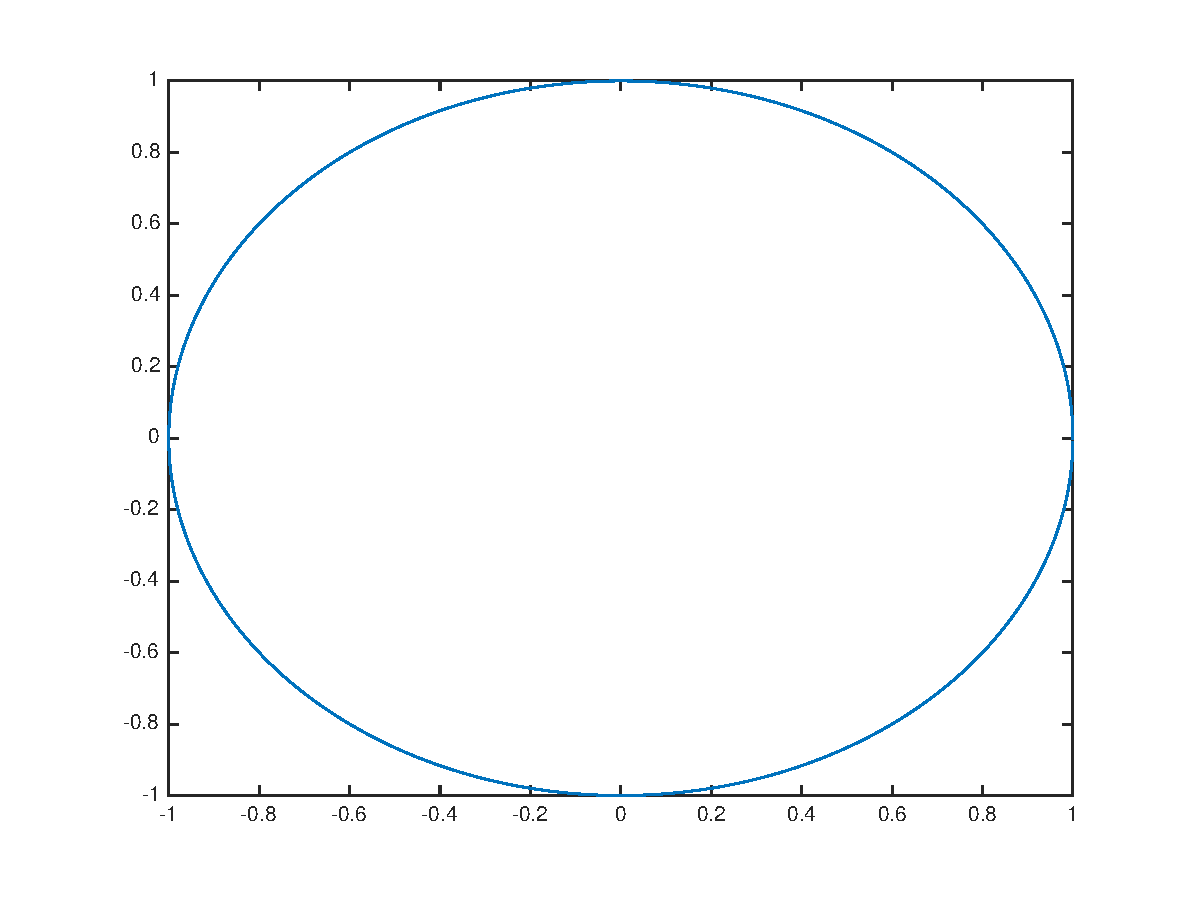
\includegraphics[width=0.48\textwidth]{./Img/figure_sc_elastic/circle.eps}
	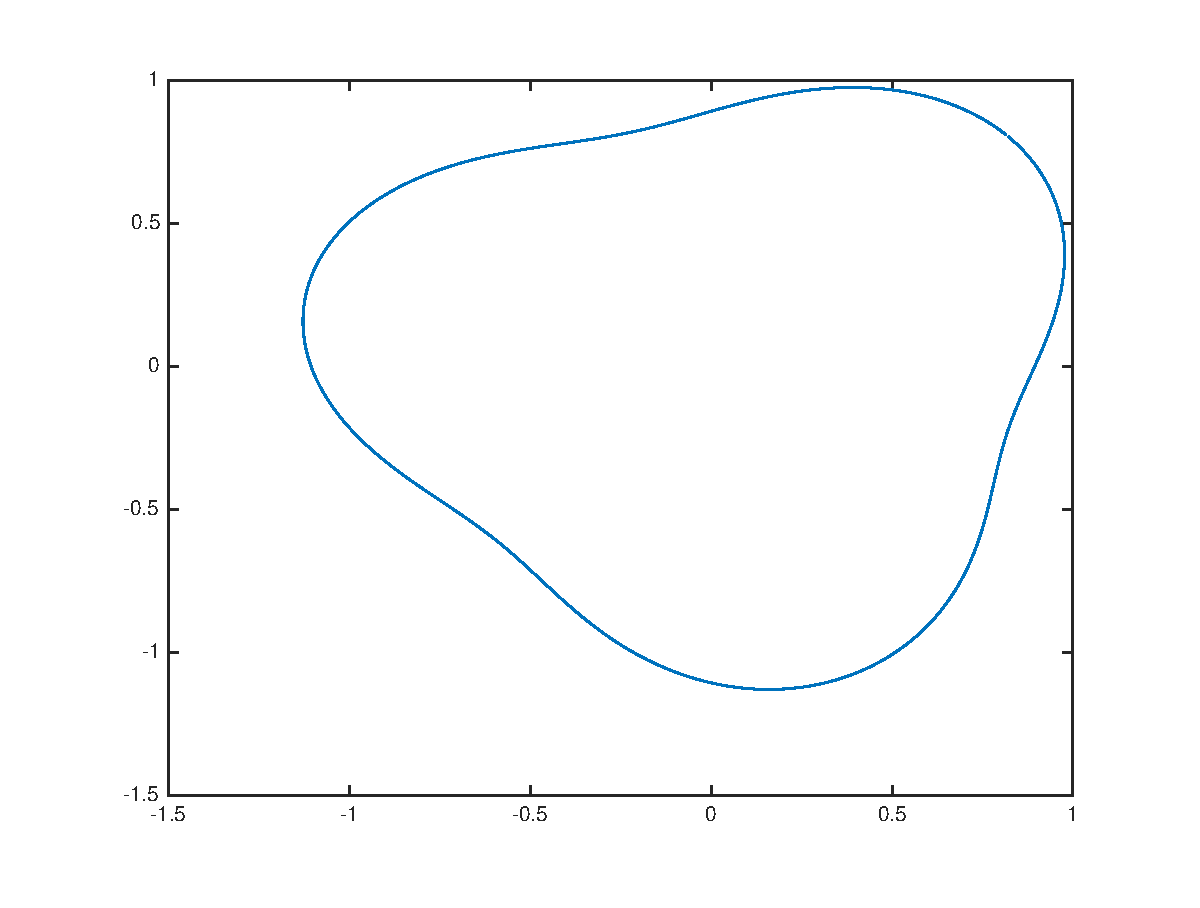
\includegraphics[width=0.48\textwidth]{./Img/figure_sc_elastic/pear.eps}
	\caption{散射系数实验中的障碍物形状:第一个是圆,第二个是梨形}\label{shape}
\end{figure}


为了比较不同角频率情况下,散射系数的逼近情况,我们分别取 $\omega= \pi,2\pi,4\pi,8\pi$。如图 \ref{figure_2}-\ref{figure_9} 所示,其中每一幅图对应某种形状的 $\mathbf{R}_\alpha^i(x;d) \ , \  \hat {\mathbf{R}}_\alpha^i(x;d,\nu(x)), \ \al=s,p,  \ i=1,2$ 的对比。
\begin{figure}[htbp]
	\centering
	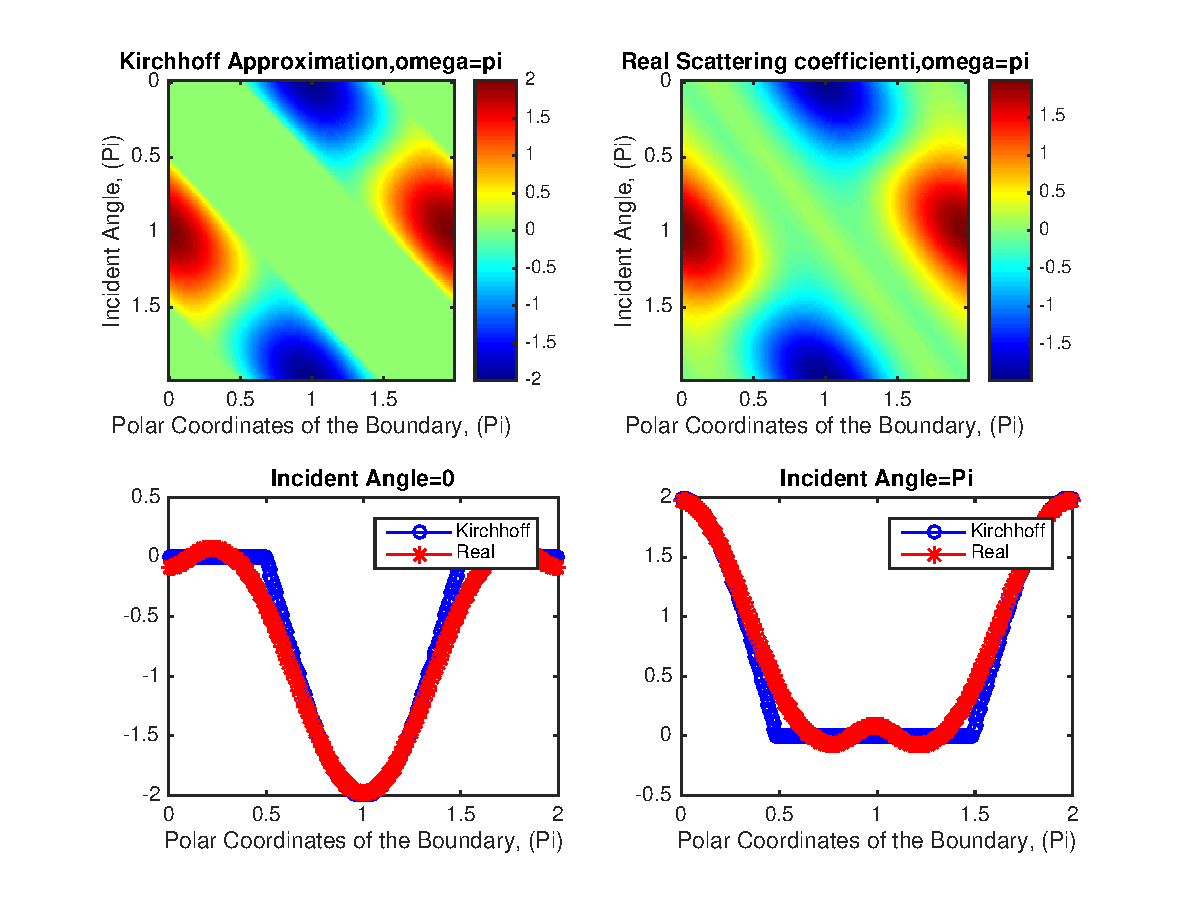
\includegraphics[width=0.48\textwidth]{./Img/figure_sc_elastic/sc_p1_circle_1.eps}
	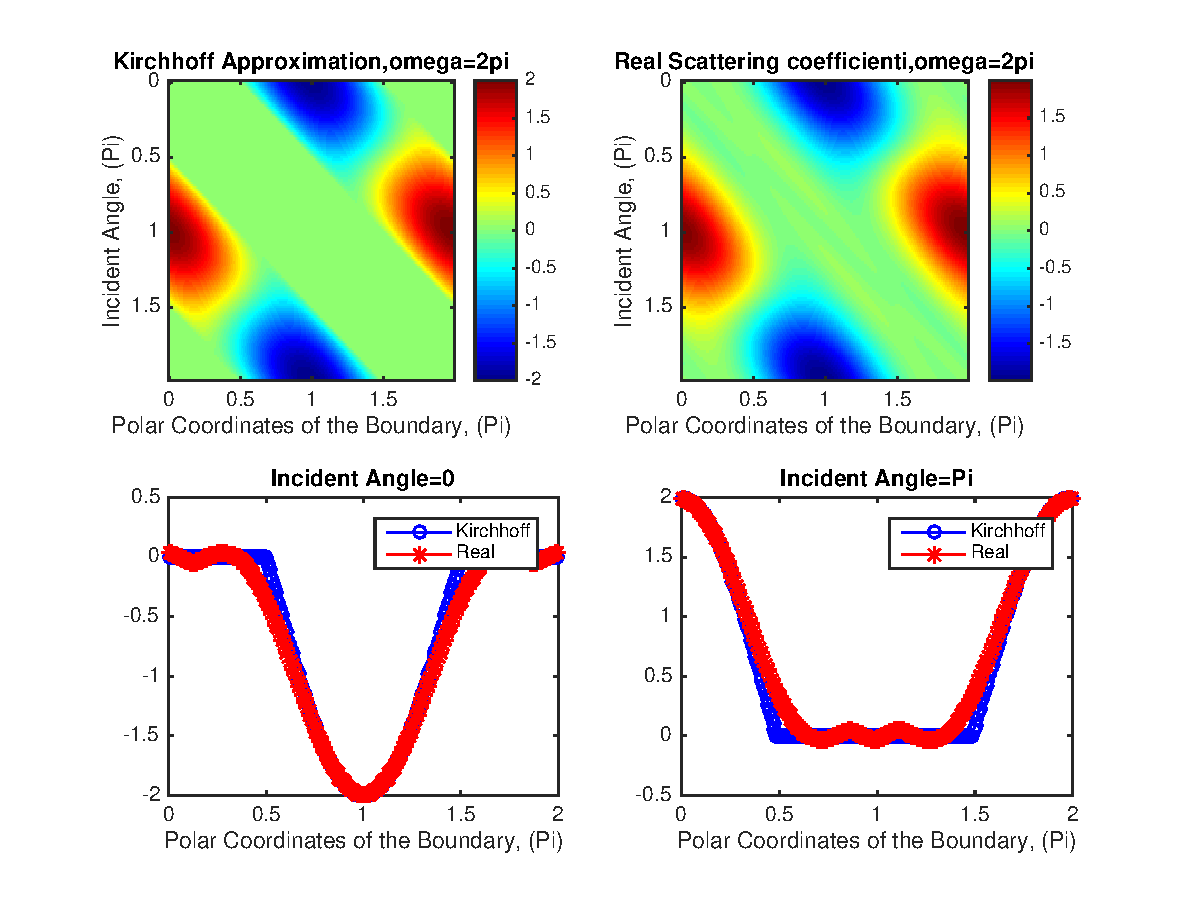
\includegraphics[width=0.48\textwidth]{./Img/figure_sc_elastic/sc_p1_circle_2.eps}
	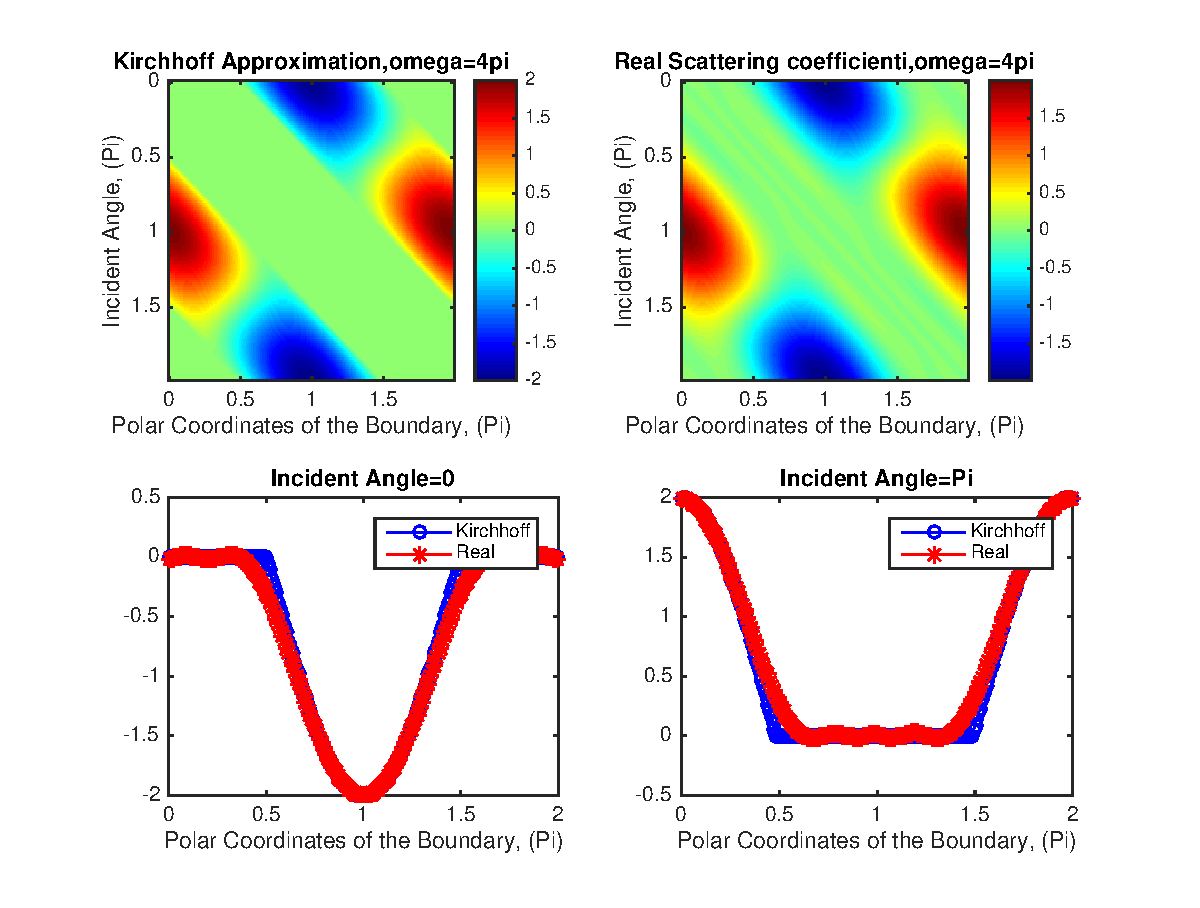
\includegraphics[width=0.48\textwidth]{./Img/figure_sc_elastic/sc_p1_circle_4.eps}
	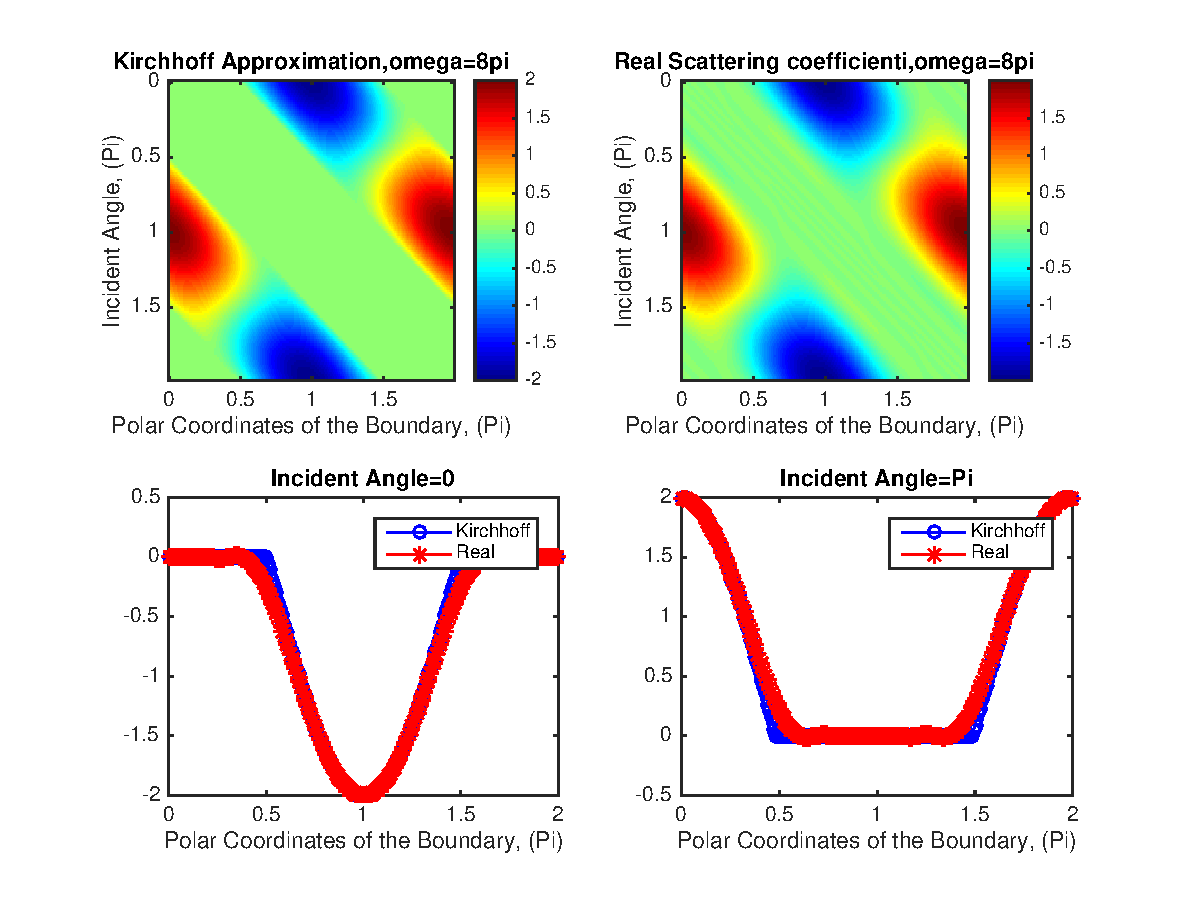
\includegraphics[width=0.48\textwidth]{./Img/figure_sc_elastic/sc_p1_circle_8.eps}		
	\caption{圆形的$\mathbf{R}_p^1$ 和 $\hat {\mathbf{R}}_p^1$ .}\label{figure_2}
\end{figure}

 每幅图含四幅针对不同角频率的子图, 每幅子图中第一行中的第一列代表真实的散射系数,第二列代表 Kirchhoff 逼近的散射系数; 第一行中的横坐标是边界的参数化 $\theta/2\pi$,纵坐标是入射方向 $t/2\pi$。第二行是入射角为 $0$ 和 $\pi$ 对于的图, 其中每幅图中红线代表真实的散射系数,蓝线代表 Kirchhoff 逼近的散射系数。
\begin{figure}[htbp]
	\centering
	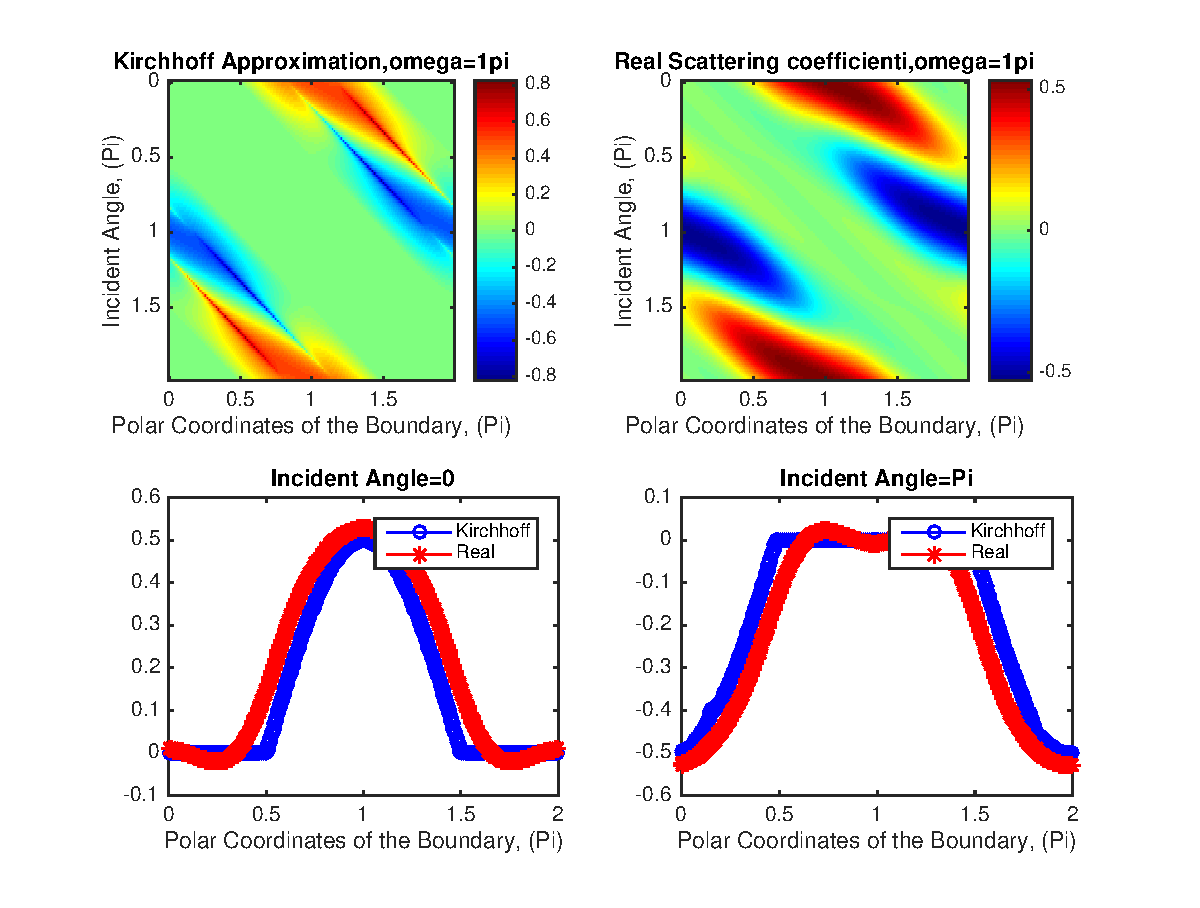
\includegraphics[width=0.48\textwidth]{./Img/figure_sc_elastic/sc_s2_circle_1.eps}
	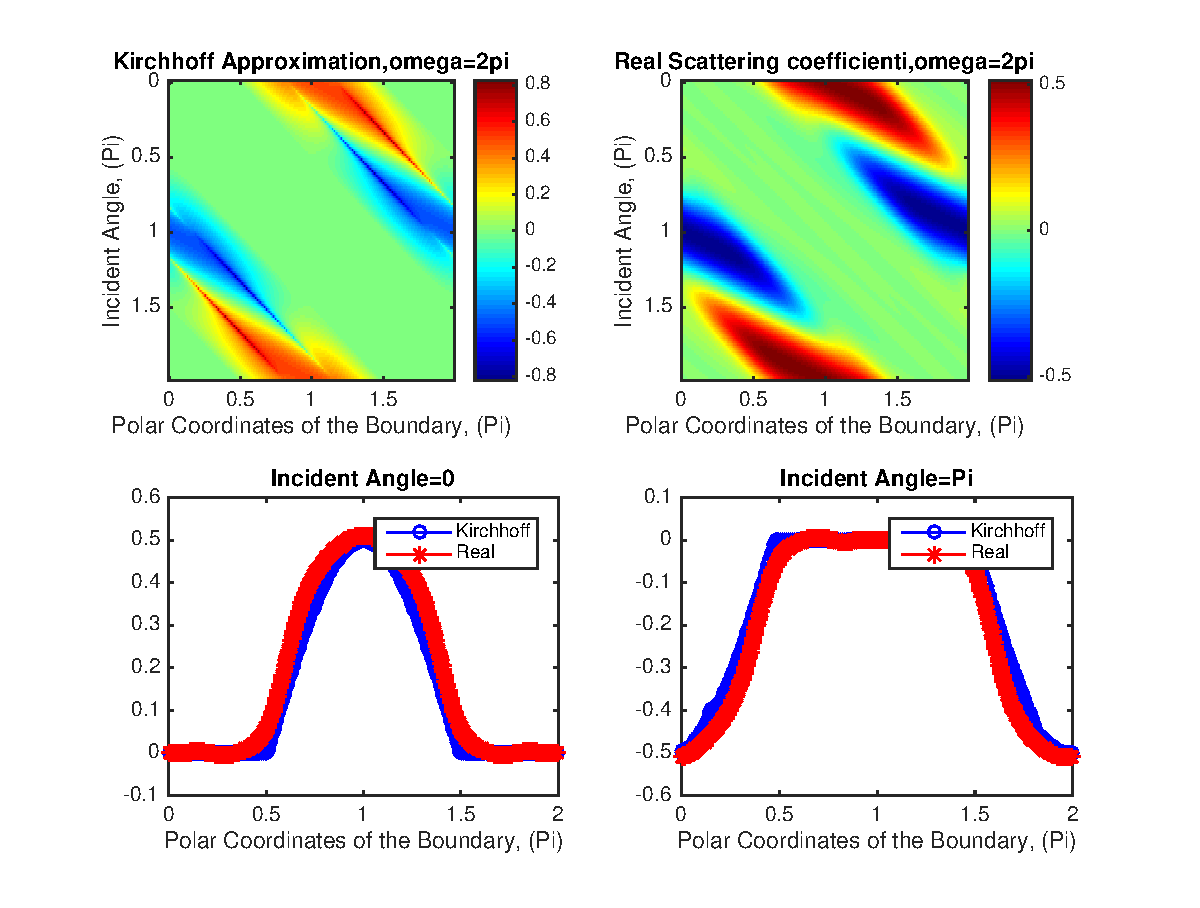
\includegraphics[width=0.48\textwidth]{./Img/figure_sc_elastic/sc_s2_circle_2.eps}
	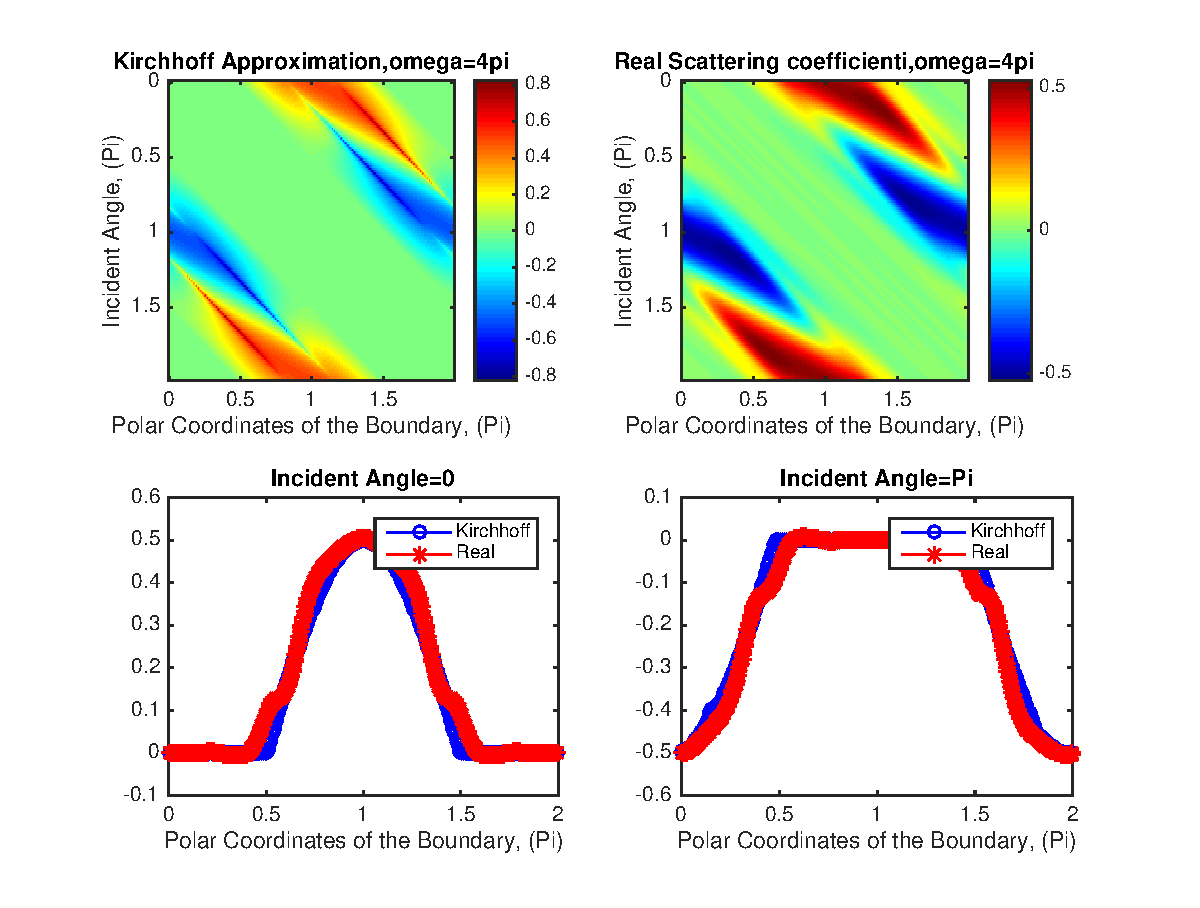
\includegraphics[width=0.48\textwidth]{./Img/figure_sc_elastic/sc_s2_circle_4.eps}
	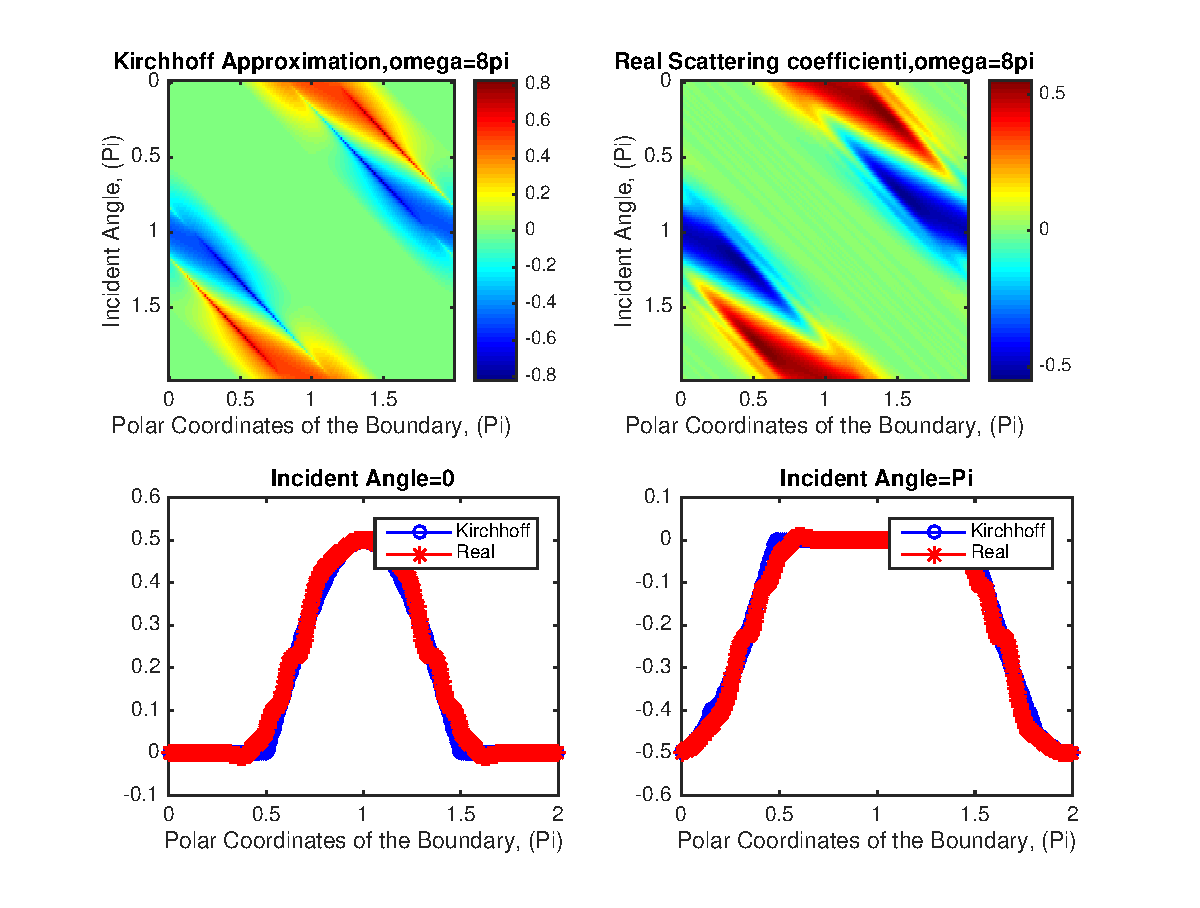
\includegraphics[width=0.48\textwidth]{./Img/figure_sc_elastic/sc_s2_circle_8.eps}		
	\caption{圆形的 $\mathbf{R}_s^2$ 和 $\hat {\mathbf{R}}_s^2$ }\label{figure_5}
\end{figure}
由图\ref{figure_2}-\ref{figure_9}, 我们可以看到, 当角频率比较大时,Kirchhoff 逼近 (\ref{kir}) 的效果是非常好, 符合高频光学近似。 然后, 我们发现当角频率不是很大的是, Kirchhoff 逼近的效果还是非常理想的。

\begin{figure}[htbp]
	\centering
	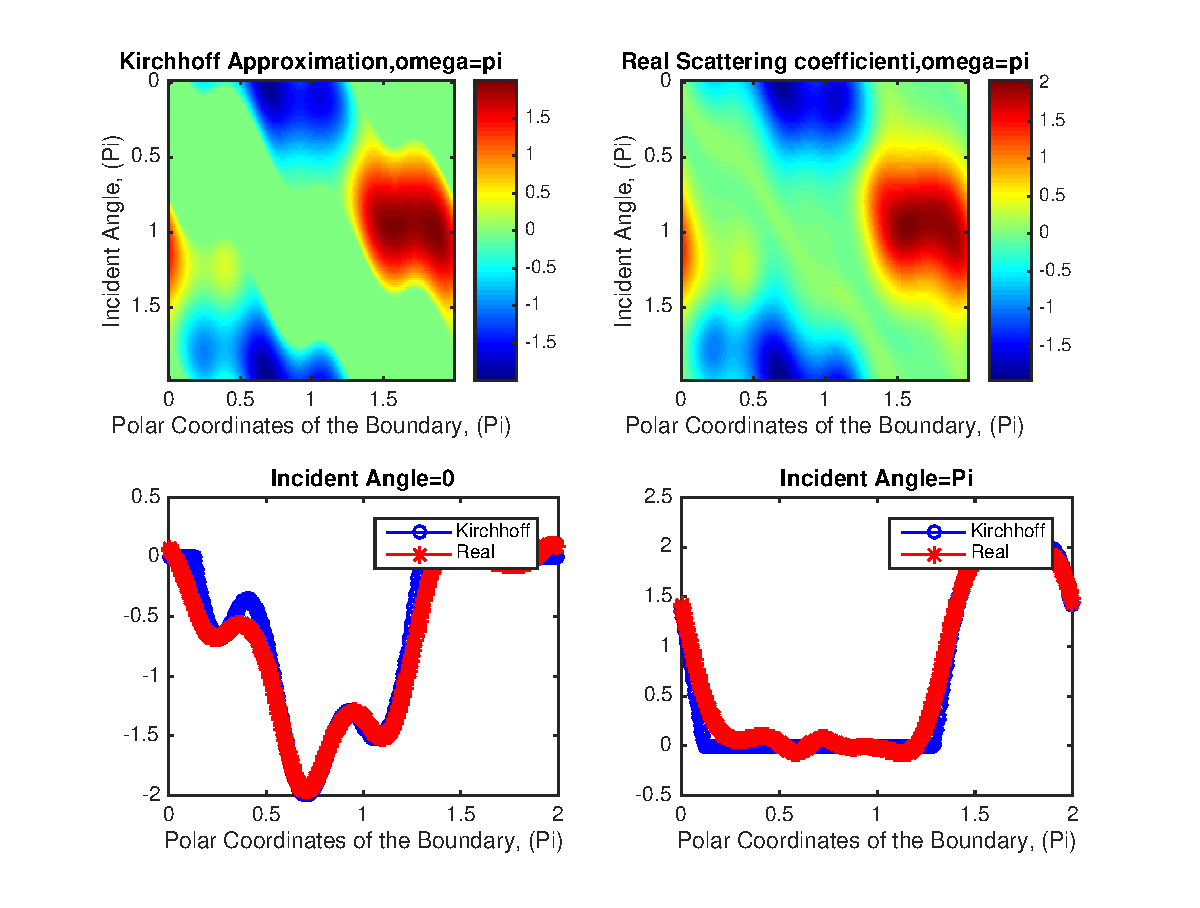
\includegraphics[width=0.48\textwidth]{./Img/figure_sc_elastic/sc_p1_pear_1.eps}
	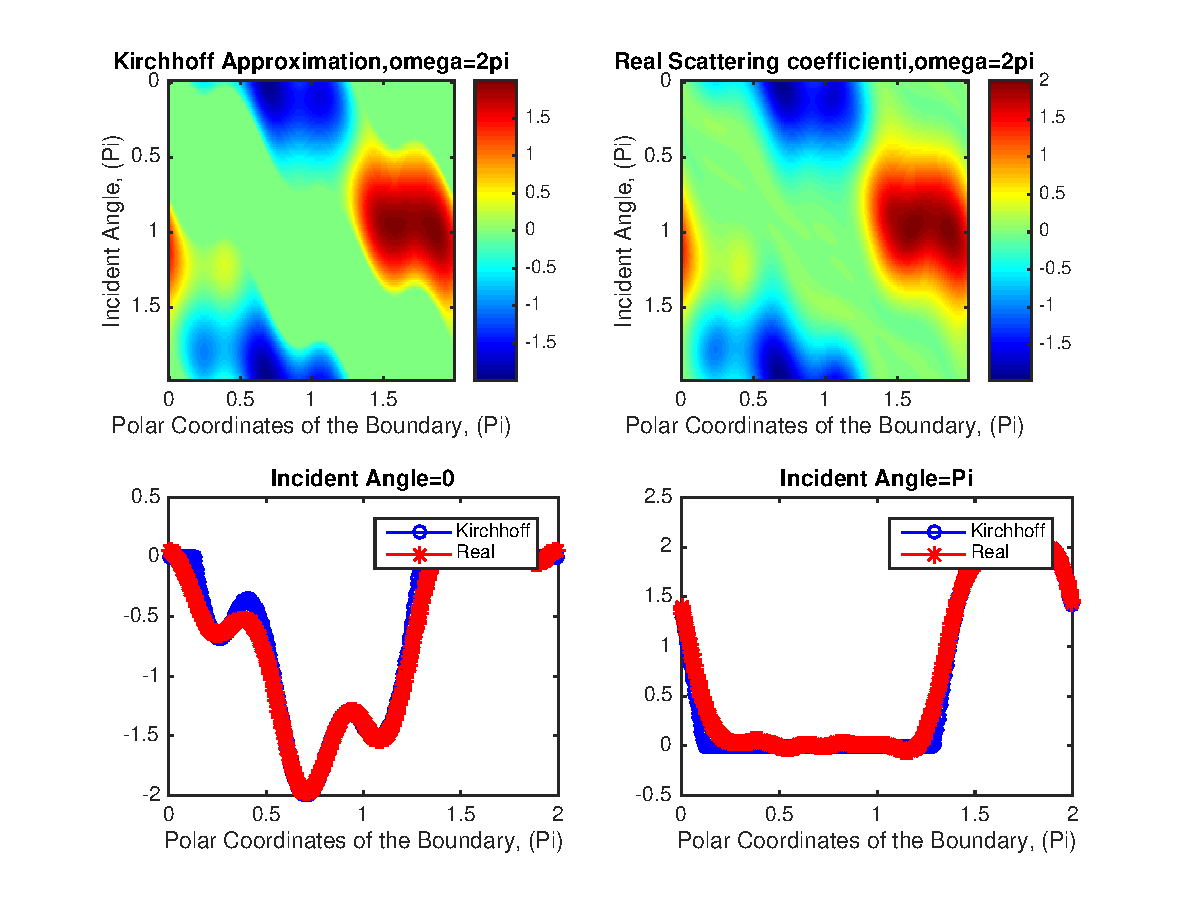
\includegraphics[width=0.48\textwidth]{./Img/figure_sc_elastic/sc_p1_pear_2.eps}
	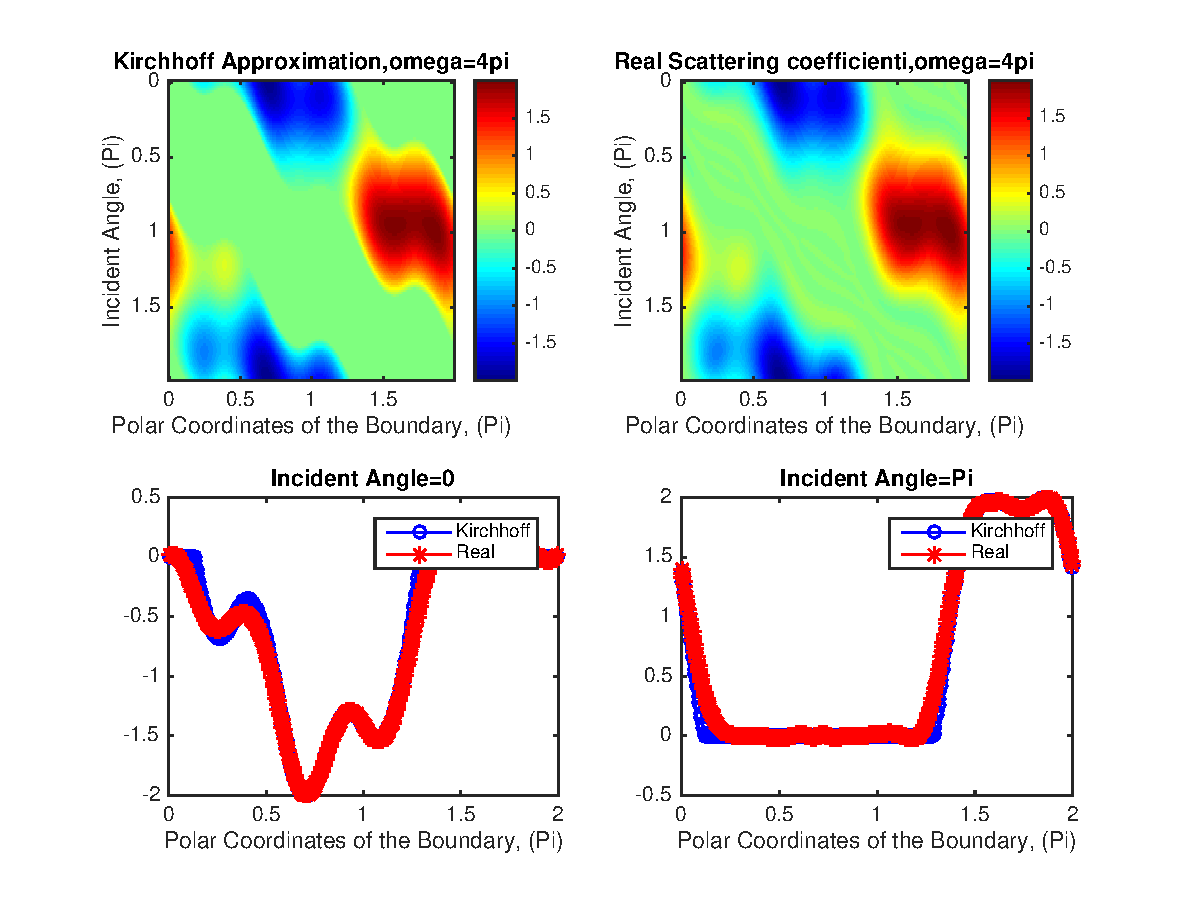
\includegraphics[width=0.48\textwidth]{./Img/figure_sc_elastic/sc_p1_pear_4.eps}
	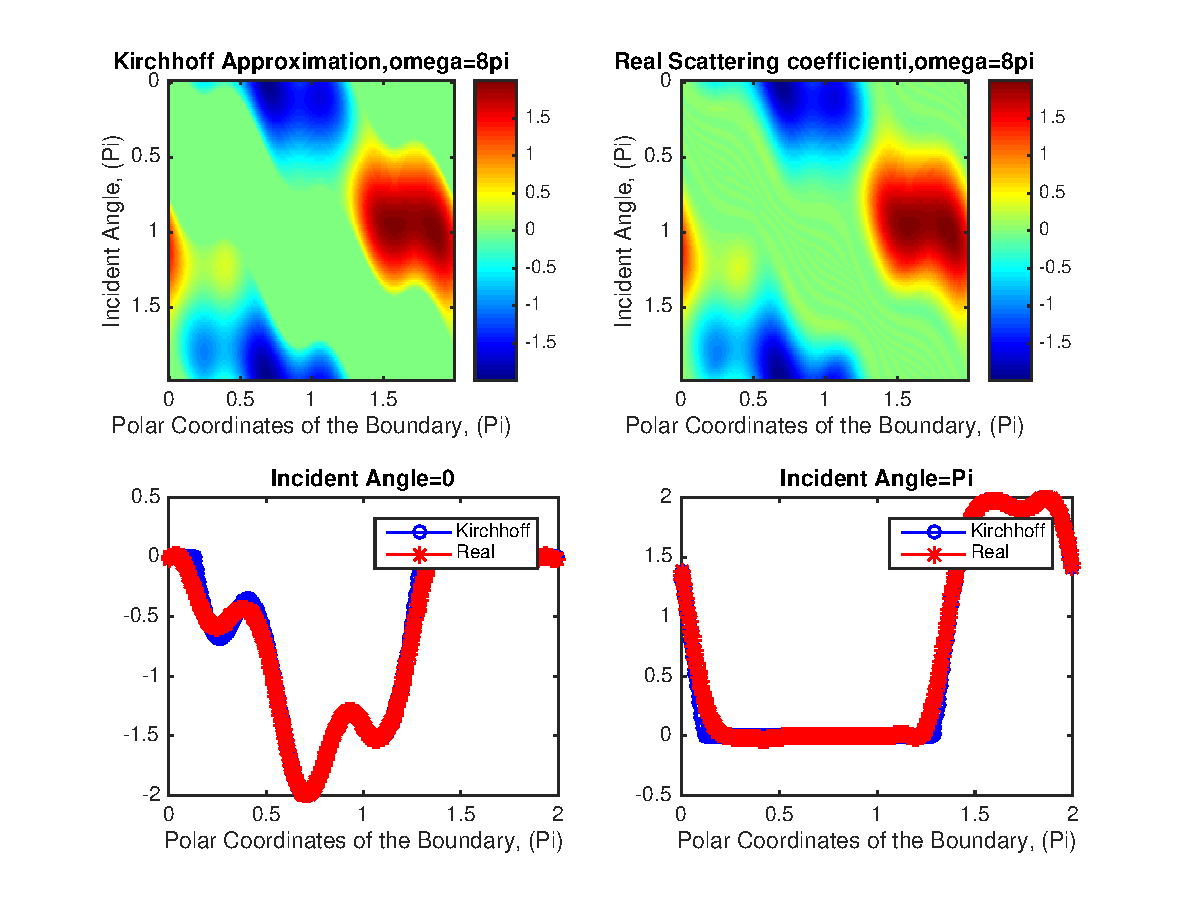
\includegraphics[width=0.48\textwidth]{./Img/figure_sc_elastic/sc_p1_pear_8.eps}		
	\caption{梨形的 $\mathbf{R}_p^1$ 和 $\hat {\mathbf{R}}_p^1$ }\label{figure_6}
\end{figure}



\begin{figure}[htbp]
	\centering
	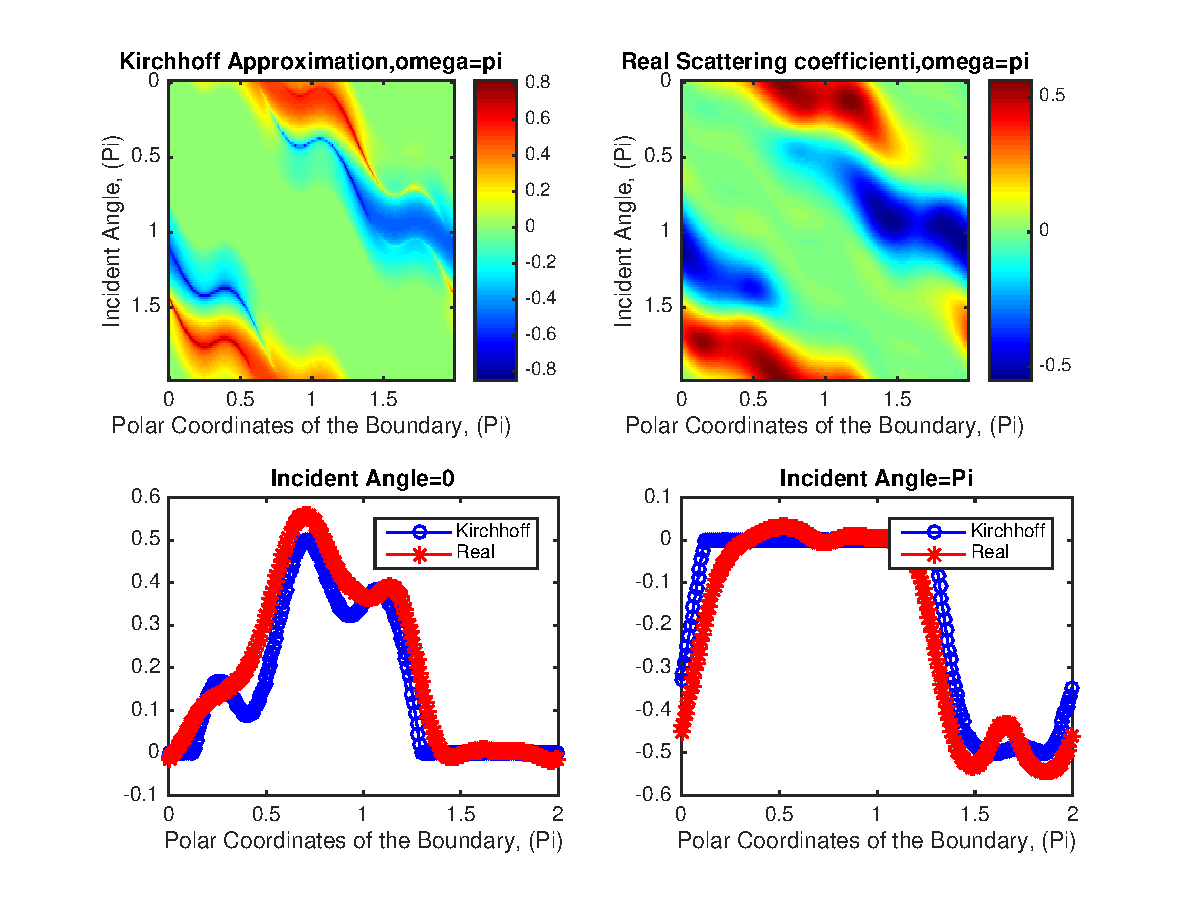
\includegraphics[width=0.48\textwidth]{./Img/figure_sc_elastic/sc_s2_pear_1.eps}
	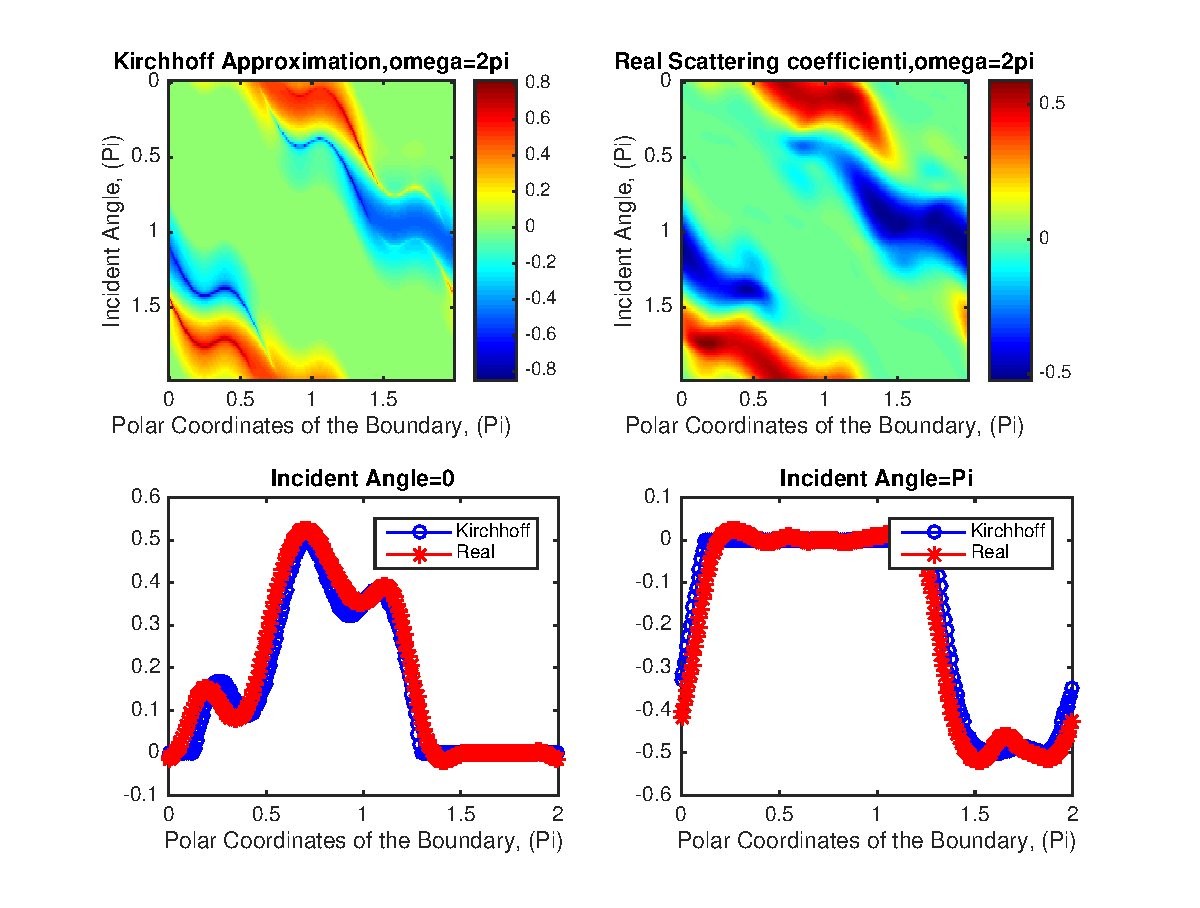
\includegraphics[width=0.48\textwidth]{./Img/figure_sc_elastic/sc_s2_pear_2.eps}
	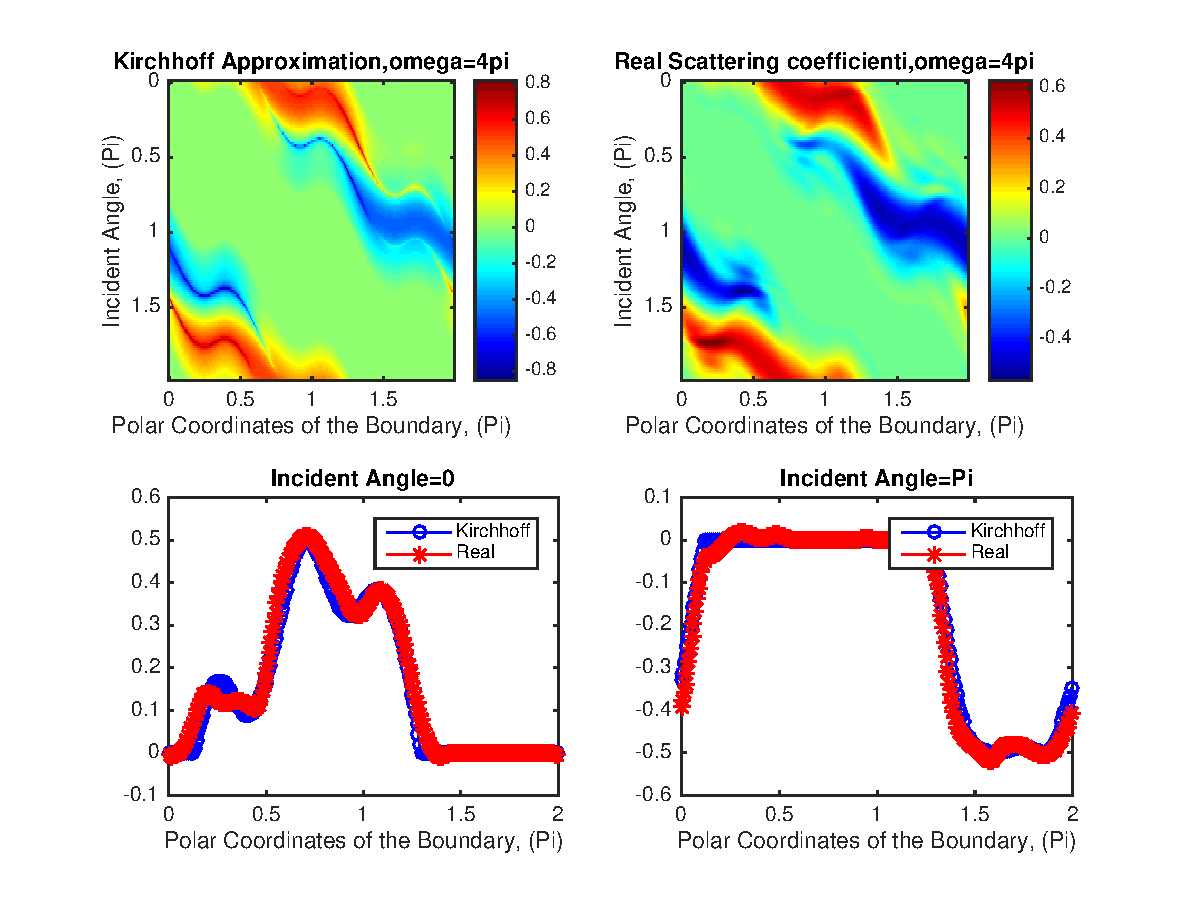
\includegraphics[width=0.48\textwidth]{./Img/figure_sc_elastic/sc_s2_pear_4.eps}
	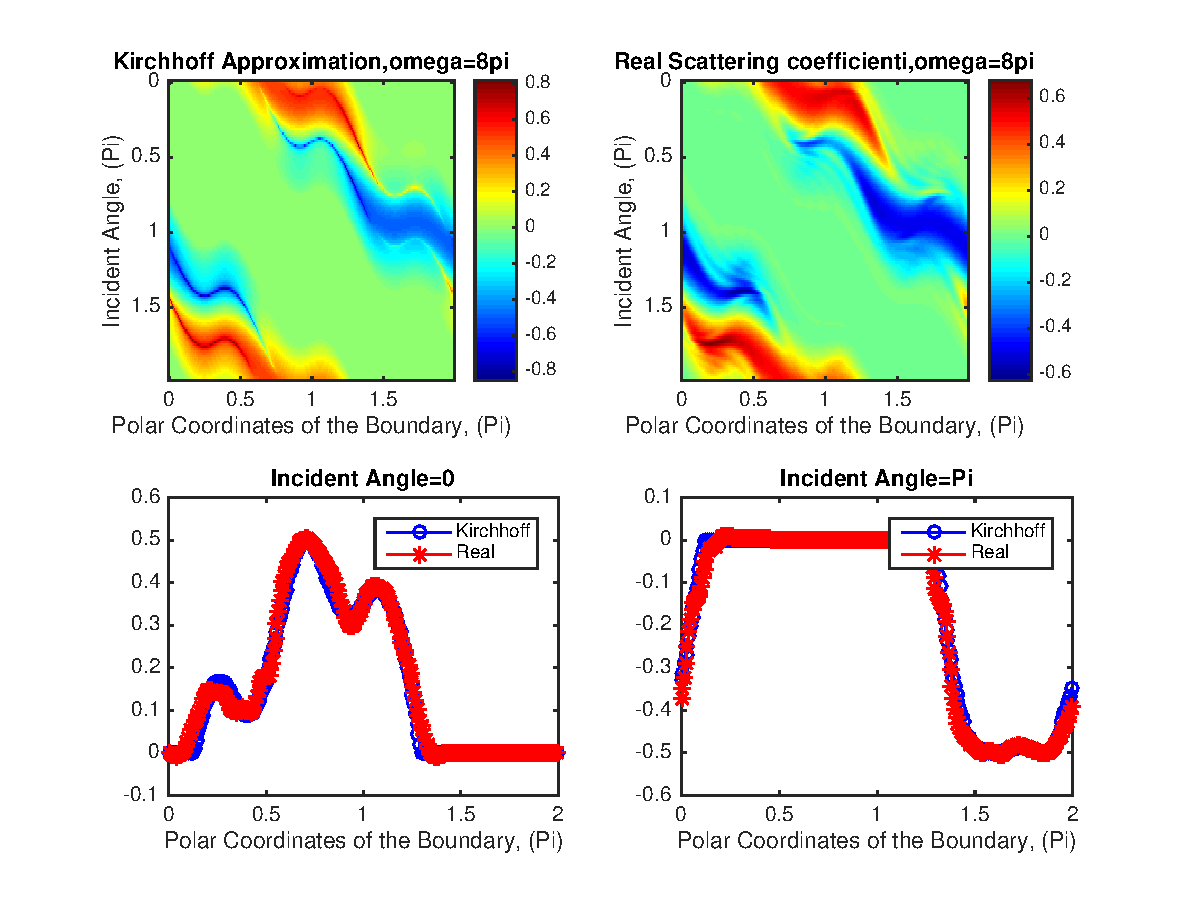
\includegraphics[width=0.48\textwidth]{./Img/figure_sc_elastic/sc_s2_pear_8.eps}		
	\caption{梨形的 $\mathbf{R}_s^2$ 和 $\hat {\mathbf{R}}_s^2$ }\label{figure_9}
\end{figure}



于是由式子 (\ref{F_theta})以及定理 \ref{thm:4.3}, 易得对于任意 $z\in\Ga_D$,
\ben
\hat I_d(z)&\approx&\Im\sum^2_{j=1}\int_{\Ga_D}\left[
\int^\pi_0\overline{\tilde A_j(\theta)}\i k_pR_p(x;\tau(\theta))e^{\i k_p(x-z)\cdot\tau(\theta)}d\theta\right]\cdot\overline{\F(z,x)}e_j ds(x)\\
& &+\Im\sum^2_{j=1}\int_{\Ga_D}\left[
\int^\pi_0\overline{\tilde B_j(\theta)}\i k_sR_s(x;\tau(\theta))e^{\i k_s(x-z)\cdot\tau(\theta)}d\theta\right]\cdot\overline{\F(z,x)}e_j ds(x).
\een
于是利用 Kirchhoff 有 
\be\label{sc4}
R_\alpha(x;\tau)\approx 0\ \ \mbox{if } x \in \Ga_D^{+}(\tau)=\{x\in \Ga_D, \nu(x)\cdot \tau>0\},\ \ \al=p,s.
\ee

 为了后文分析, 我们引入下面著名的驻相引理, 见  \cite[Theorem 7.7.5]{hor}.
 \begin{lem}\label{phase}
 	令振幅函数 $g\in C^2_0(\R)$ 及相函数 $f\in C^2(\R)$ 存在驻相点 $t_0$ ,即为 $f'(t_0)=0$, $f''(t_0)\not=0$, 且当 $t\not=t_0$ 时有 $f'(t)\not=0$ 。 于是对于任意 $\lambda>0$,存在常数 $C$ 成立
 	\ben
 	\left|\int_{\R}g(t)e^{\i\lambda f(t)}dt-g(t_0)e^{\i\lambda f(t_0)}\left(\frac{\lambda f''(t_0)}{2\pi\i}\right)^{-1/2}\right|
 	\le C\lambda^{-1}\|g''\|_{C(\R)}.
 	\een
 \end{lem}

 这里,我们假设障碍物 $D$ 是凸的 。令 $x(s)$, $0<s<L$, 是障碍物边界 $\Ga_D$ 的关于弧长的参数化表示。 定义 $x_{\pm}(\theta)$ 是边界 $\Ga_D$ 上满足 $\nu(x_\pm(\theta))=\pm\tau(\theta)$ 的点。令相函数 $f(s)= (x(s)-z)\cdot\tau(\theta)$ 且有 
 \ben
 f'(s)=x'(s)\cdot\tau(\theta),  \ \ f''(s)=x''(s) \cdot\tau(\theta).
 \een
 显然有 $f'(s_\pm)=\pm x'(s_\pm)\cdot\nu(x(s_\pm)), f''(s_\pm)=\pm x''(s_\pm)\cdot \nu(yx(s_\pm))= \pm\kappa(x(s_\pm))|x'(s_\pm)|^2$, 其中 $\kappa$ 表示 $\Ga_D$ 的曲率。
因此,利用驻相引理和 Kirchhoff 逼近 (\ref{sc4}) 我们可以得到:
\ben
\hat I_d(z)&\approx&\Im\sum^2_{j=1}\sqrt{2\pi k_p}
\int^\pi_0\overline{\tilde A_j(\theta)}e^{\i k_p(x_-(\theta)-z)\cdot\tau(\theta)+\i\frac\pi 4}\,\frac{R_p(x_-(\theta);\tau(\theta))\cdot\overline{\F(z,x_-(\theta))}e_j}{\sqrt{\kappa(x_-(\theta))}}d\theta\\
& &+\Im\sum^2_{j=1}\sqrt{2\pi k_s}
\int^\pi_0\overline{\tilde B_j(\theta)}e^{\i k_s(x_-(\theta)-z)\cdot\tau(\theta)+\i\frac\pi 4\,}\frac{R_s(x_-(\theta);\tau(\theta))
	\cdot\overline{\F(z,x_-(\theta))}e_j}{\sqrt{\kappa(x_-(\theta))}}d\theta.
\een
由于 $\nu(x_-(\theta))=-\tau(\theta)$, 通过 (\ref{kir_p}) 和 (\ref{kir_s}) 我们可以得到
\be\label{sc5}
& &R_p(x_-(\theta);\tau(\theta))\approx-2(\lam+2\mu)\tau(\theta),\ \ \\ 
\label{sc6} & &R_s(x_-(\theta);\tau(\theta))\approx-2\mu\tau(\theta)^\perp.
\ee

现在, 我们来观察边界 $\Ga_D$ 上的点 $z$。 当$\nu(z)\cdot\tau(\theta)>0$ 时,其中 $\theta\in (0,\pi)$, 此时 $z$ 点位于 $\Ga_D$ 背对于 $\Ga_0$ 的那一部分。同时,此时 $x_-(\theta)$ 位于 $\Ga_D$ 正对于 $\Ga_0$ 的那一部分。 于是, $z$ 距离 $x_-(\theta)$ 就较远, 因此得到 $\F(z,x_-(\theta))e_j\approx 0$, 然后有  $\hat{I}_d(z)\approx0$。 这就说明,只利用 $\Ga_0$ 上收集的数据无法将障碍物背对于 $\Ga_0$ 那部分成像, 而且这一结论在后文中的数值算例中也得到证实。 
另一方面, 如果 $z$ 位于 $\Ga_D$ 正对于 $\Ga_0$ 的阳面, 利用 (\ref{sc5}),(\ref{sc6}) , 我们可以发现 $\hat I_d(z)$ 正是 $[\kappa(x_-(\theta))]^{-1/2}$ 的加权和, 其中 $x_-(\theta)$ 在$\Ga_D$ 上 $z$ 附近的那部分点。综上所述, 成像函数 $\hat{I}_d(z)$ 可以将障碍物边界成像, 且仅能将障碍物的阳面成像。


\section{其它类型障碍物的RTM分辨率分析}
在这一节中, 我们将考虑在半空间弹性介质中利用 RTM 算法 \ref{alg_rtm} 来重构具有阻抗边界条件的不可穿透障碍物和可穿透障碍物。

对于具有阻抗边界的不可穿透的障碍物,我们接收到的测量数据为 $u_q(x_r,x_s)=u_q^s(x_r,x_s)+\N(x_r,x_s)q$, $q=e_1, e_2$, 其中 $u^s_q(x,x_s)$ 是如下半空间弹性波方程的散射解:
\ben
& &\Delta_e u^s_q(x,x_s) + \omega^2 u^s_q(x,x_s) =0\ \ \mbox{\rm in } \R^2_+\bks \bar{D}, \\
& &\sigma(u^s_q(x,x_s))\nu+\i\eta(x)u^s_q(x,x_s)=-[\sigma(\N(x,x_s)q)\nu+\i\eta(x)\N(x,x_s)q]\ \ \mbox{\rm on } \Ga_D, \\ 
& &\sigma(u^s_q(x,x_s))e_2=0 \ \ \mbox{\rm on } \Ga_0,
\een
这里在 $\Ga_D$ 上 $\eta\in L^\infty(\Ga_D)$ 以及 $\eta\ge 0$,特别地, 当 $\eta=0$ 时, 上面的障碍物边界条件对应的是 Neumann边界条件,因此这里我们不在单独讨论满足 Neumann 边界条件的障碍物。 对定理 \ref{thm:4.3} 稍作修改, 我们可以得到如下针对具有阻抗边界的不可穿透型障碍物的 RTM 方法的分辨率分析的定理, 这里我们不在赘述定理证明。
\begin{thm}\label{thm:5.1}
	对于任意 $z\in\Omega$, 令 $\U(z,x)\in\C^{2\times2}$, 其中 $\U(z,x)e_j$, $j=1,2$ 是如下弹性波方程的散射解:
	\ben
	\hskip-1cm& & \Delta_e[\U(z,x)e_j]+ \omega^2[\U(z,x) e_j]= 0 \ \ \mbox{\rm in }\R^2\bks \bar{D},\\
	\hskip-1cm& &\sigma(\U(z,x)e_j)\nu+\i\eta(x)[\U(z,x)e_j]= -[\sigma(\overline{\F(z,x)}e_j)\nu+\i\eta(x)\overline{\F(z,x)}e_j ]\ \ \mbox{\rm on} \ \Ga_D.
	\een
	于是针对具有阻抗边界的不可穿透障碍物的散射数据 $u^s_q(x_r,x_s)$,RTM 成像函数(\ref{cor2}) 有如下表示
	\ben
	\hat{I}_d(z)&=&-\Im\sum_{j=1}^2\int_{\Gamma_D} [\U(z,x)e_j+\overline{\F(z,x)}e_j]\cdot[\sigma(\overline{\F(z,x)}e_j)\nu+\i\eta(x)\overline{\F(z,x)}e_j]ds(x)\ \\
	& &+R_d(z),\ \ \ \ \ \ \ \ \forall z\in\Om,
	\een
	这里 $|R_d(z)|\leq C\mu^{-2}(1+k_s d_D)^3\left[\left(\frac hd\right)^{2}+(k_sh)^{-1/4}\right]$ 其中常数 $C$ 仅依赖于 $\kappa$ 而与 $k_s,k_p, h, d, d_D$ 无关。
\end{thm}

对于可穿透型障碍物, 我们接收到的测量数据为 $u_q(x_r.x_s)=u_q^s(x_r,x_s)+\N(x_r,x_s)q$, $q=e_1,e_2$, 其中 $u^s_q(x,x_s)$ 是如下弹性波方程的散射解:
\ben
& &\Delta_e u^s_q(x,x_s) + \omega^2n(x) u^s_q(x,x_s) =-\om^2(n(x)-1)\N(x,x_s)q\ \ \mbox{\rm in } \R^2_+, \\
& &\sigma(u^s_q(x,x_s))e_2=0 \ \ \mbox{\rm on }\Ga_0, 
\een
这里 $n(x)\in L^{\infty}({\R^2_+})$ 是正函数,且当 $x\notin D$ 时,$n(x)==1$。类似地, 对定理 \ref{thm:4.3} 稍作修改, 我们可以得到如下针对可穿透型障碍物的 RTM 方法的分辨率分析的定理, 这里我们不在赘述定理证明。

\begin{thm}\label{resolution2}
	对于 $z\in\Omega$, 令 $\U(z,x)\in\C^{2\times2}$ 其中 $\U(z,x)e_j$, $j=1,2$ 是如下弹性波方程的散射解:
	\ben
	& & \Delta_e [\U(z,x)e_j] + \omega^2n(x)[\U(z,x)e_j]= -\omega^2(n(x)-1)\overline{\F(z,x)}e_j \ \ \mbox{\rm in }\R^2.
	\een
	于是针对可穿透型障碍物的散射数据 $u^s_q(x_r,x_s)$,RTM 成像函数(\ref{cor2}) 有如下表示
	\ben
	\hat{I}_d(z)=\Im\sum_{j=1}^2 \int_{D}\omega^2(n(x)-1)[(\U(z,x)e_j+\overline{\F(z,x)}e_j)\cdot\overline{\F(z,x)}e_j]dx+R_d(z),
	\een
	这里 $|R_d(z)|\leq C\mu^{-2}(1+k_s d_D)^3\left[\left(\frac hd\right)^{2}+(k_sh)^{-1/4}\right]$ 其中常数 $C$ 仅依赖于 $\kappa$ 而与 $k_s,k_p, h, d, d_D$ 无关。
\end{thm}


\section{数值测试}

在这一节中, 我们将呈现若干数值实验来展示 
RTM 算法的有效性。 为了合成散射数据, 我们对要计算的半空间弹性波方程的散射解 $u^s_q(x,x_s)$ 表示成以 Neumann Green 函数 $\N(x,y)$ 为积分核的单层位势,然后通过 Dirichlet 边界条件,与入射波 $u^i_q(x,x_s)$ 组合成边界积分方程。
由于当$ x=y$ 时,Neumann Green 函数 $\N(x,y)$ 只具有弱奇异性,即$\log |x-y|$。于是, 我们可以利用 Nystr\"{o}m 方法 \cite{colton-kress} 来离散边界 $\Ga_D$ 上的积分方程。 针对边界的离散剖分, 我们采用一致网格, 且每一个 p 入射波长均匀设置 10 个网格点。发射器和接收器均匀地分布在 $\Ga_d$ 上, 且对于所有数值实验, 都取 $h = 10, d = 50$ 及 {Lam\'{e}} 常数 $\lambda=1/2$, $\mu=1/4$。 下面实验中的各种障碍物形状, 其边界参数化表示如下: 
\ben
\mbox{圆形:}\ \ \ \ &&x_1=\rho\cos(\theta),\ \ x_2=\rho\sin(\theta);\ \ \\
\mbox{风筝形:}\ \ \ \ &&x_1=\cos(\theta) + 0.65\cos(2\theta) - 0.65,\ \ x_2=1.5 \sin (\theta);\ \ \\
\mbox{$p$-叶形:}\ \ \ \ &&r(\theta)=1+0.2\cos(p\theta); \\
\mbox{花生形:}\ \ \ \ &&x_1 = \cos \theta + 0:2 \cos 3\theta; x_2 = \sin \theta + 0:2 \sin 3\theta; \\
\mbox{方形:}\ \ \ \ &&x_1 = \cos3 \theta + \cos \theta; x_2 = \sin3\theta + \sin \theta.
\een
这里
$\theta\in[0,2\pi]$。且这里的数值成像函数为:
\ben
I_d(z)=\Im\sum_{q=e_1,e_2}\left\{\frac{|\Gamma_0^d|^2}{N_sN_r}\sum^{N_s}_{s=1}\sum^{N_r}_{r=1}
[\T_D(x_s,z)^Tq]\cdot[\T_D(x_r,z)^T\overline{u^s_q(x_r,x_s)}]\right\}.
\een

\bigskip

在下文中,我们所谓的 Dirichlet, Neumann 或是阻抗 (Impedance) 障碍物, 就意味着该障碍物是不可穿透的,而且其边界 $\Ga_D$ 满足 Dirichlet, Neumann 或是 阻抗边界条件。


\bigskip
\textbf{算例 1}. 这里我们只考虑  Dirichlet 障碍物来成像, 而变量是障碍物的形状, 包括圆形,花生形,四叶草形 以及旋转后的方形。 同样地, 
我们考虑针对 Dirichlet 障碍物,  Neumann 障碍物, 阻抗障碍物, 以及可穿透障碍物进行成像。 每个成像区域都为 $\Om=(-2,2) \times (8, 12)$ 且其样本点网格取为 $201 \times 201$。 我们设置发射器和接收器数量为 $N_s = N_r = 401$。 这里针对单频, 我们取角频率 $\om = 3\pi,4\pi$ ; 针对多频,取 $\om=\pi\times[2:0.5:8]$ ,再将成像函数值叠加。
\begin{figure}[htbp]
	\centering
	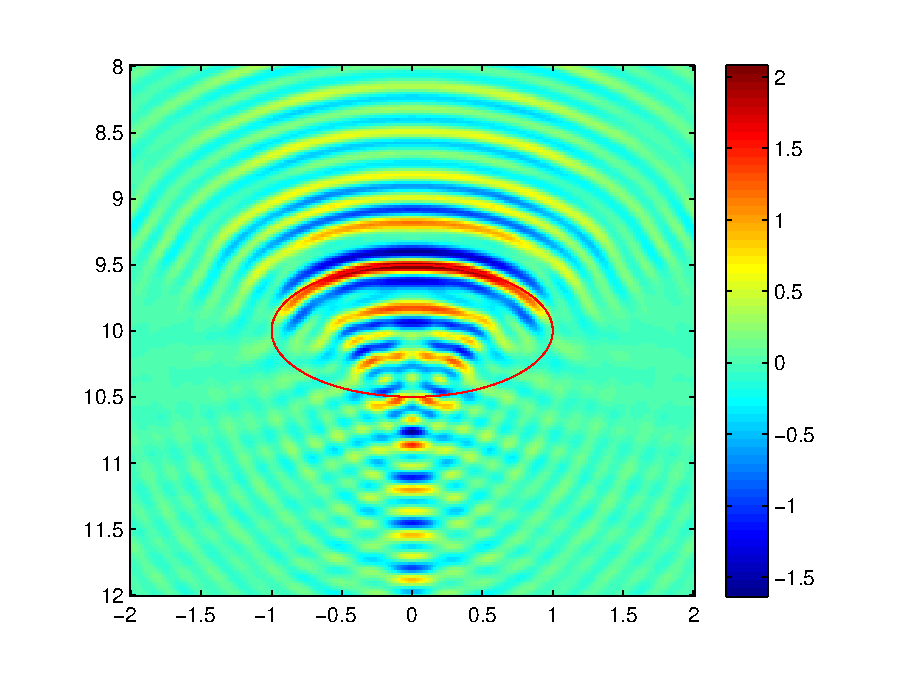
\includegraphics[width=0.32\textwidth]{./Img/graphic/circle_3pi.eps}
	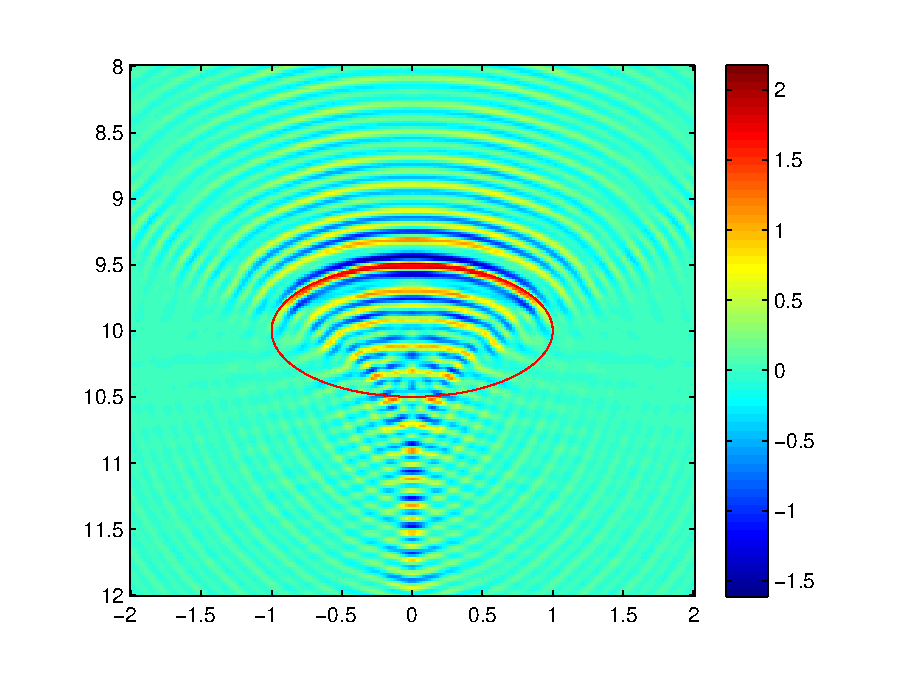
\includegraphics[width=0.32\textwidth]{./Img/graphic/circle_5pi.eps}
	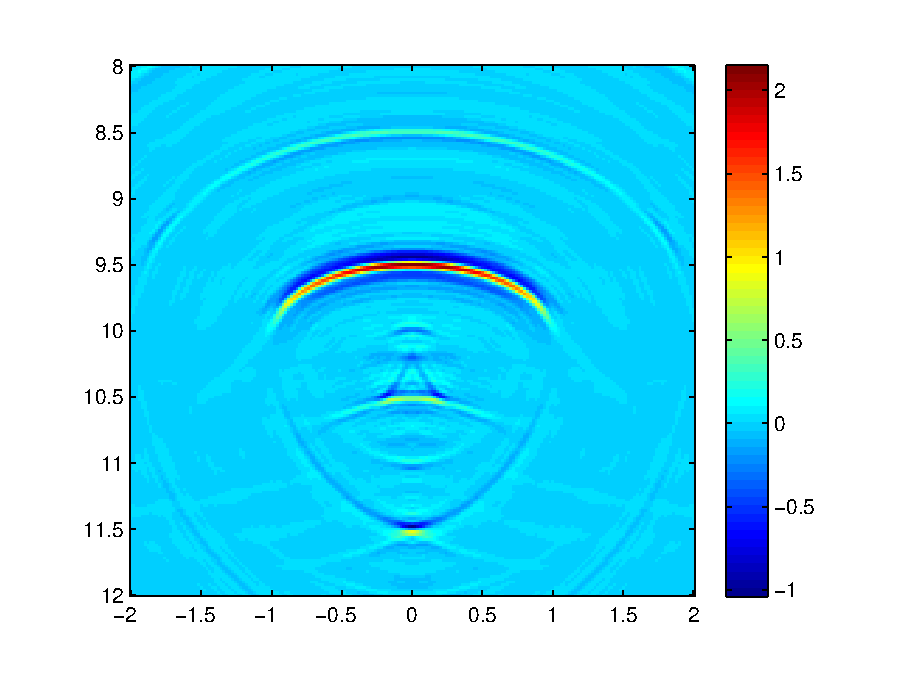
\includegraphics[width=0.32\textwidth]{./Img/graphic/circle.eps}
	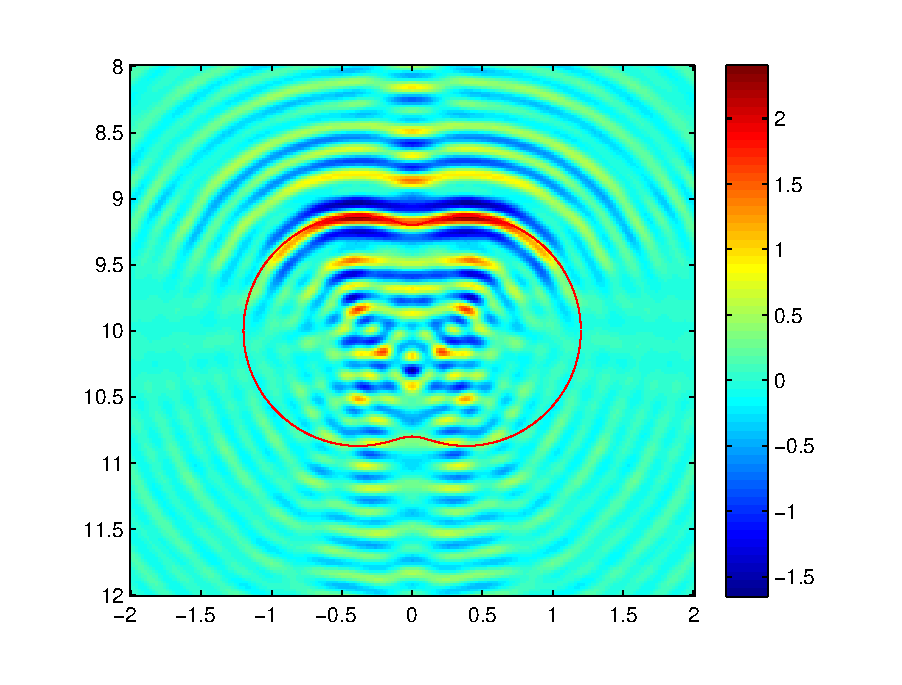
\includegraphics[width=0.32\textwidth]{./Img/graphic/peanut_3pi.eps}
	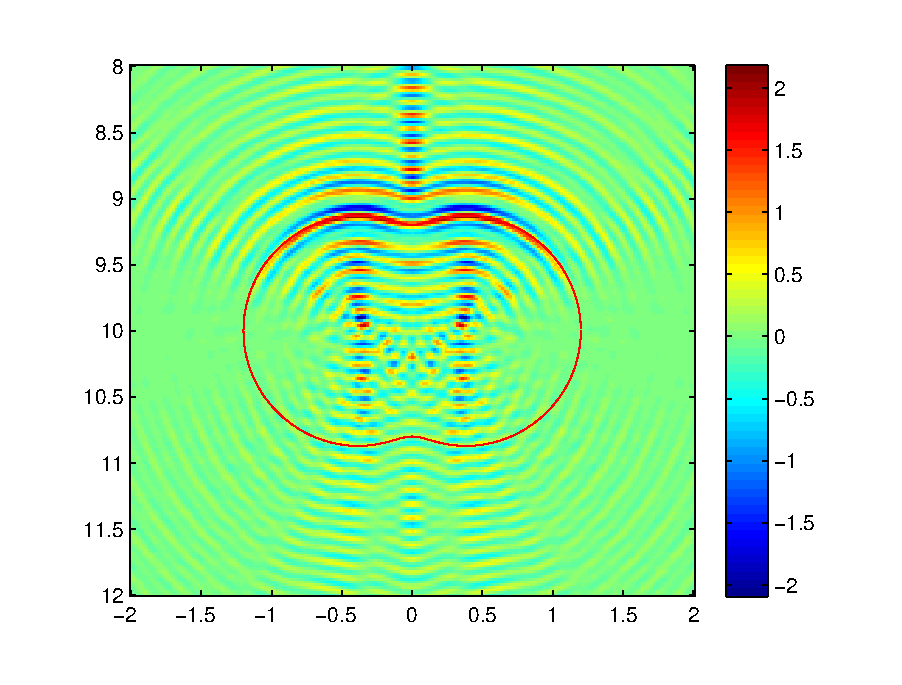
\includegraphics[width=0.32\textwidth]{./Img/graphic/peanut_5pi.eps}
	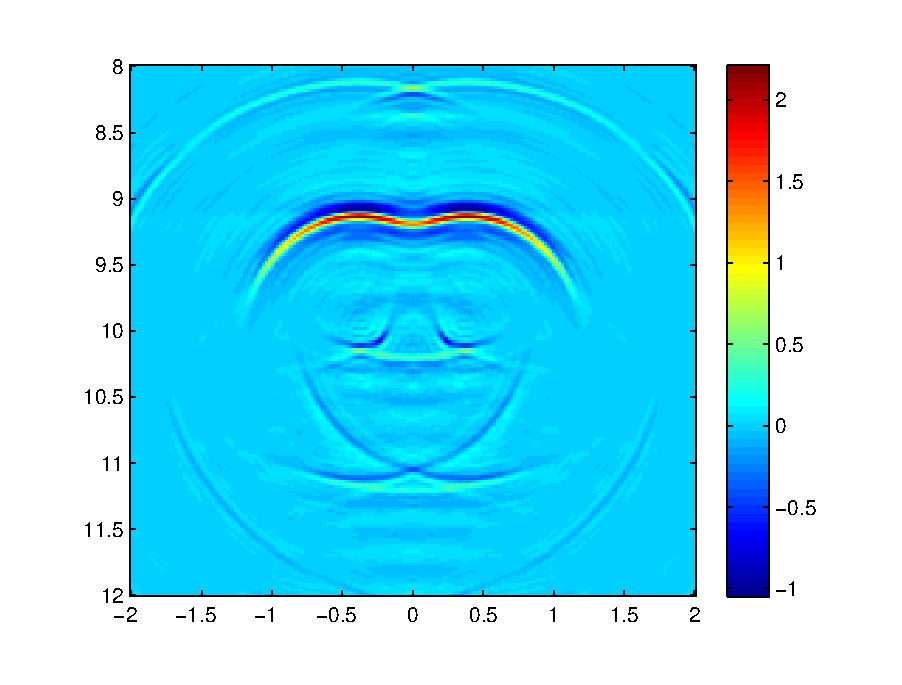
\includegraphics[width=0.32\textwidth]{./Img/graphic/peanut.eps}
	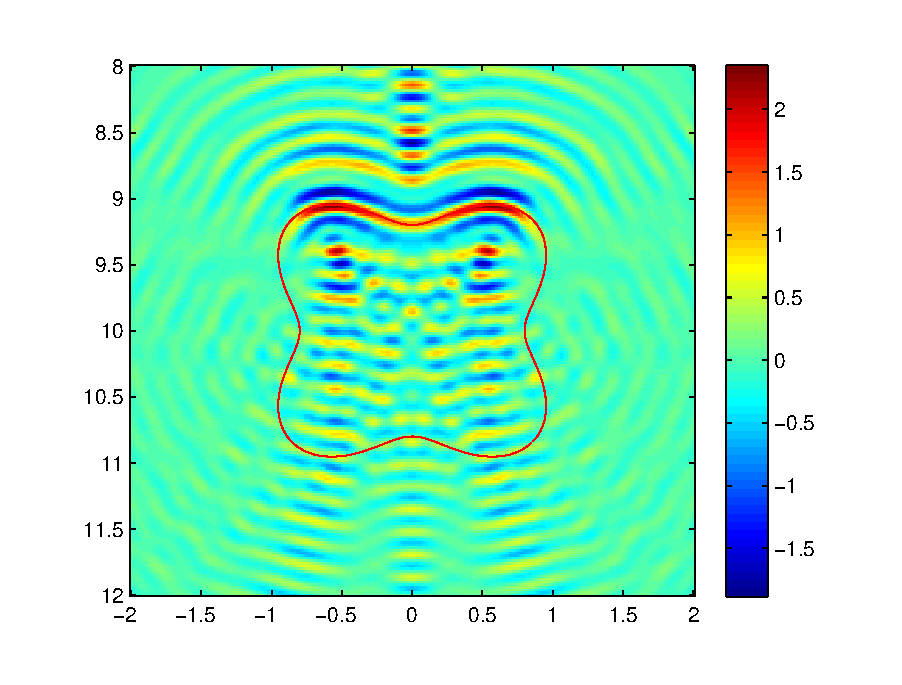
\includegraphics[width=0.32\textwidth]{./Img/graphic/p_leaf_3pi.eps}
	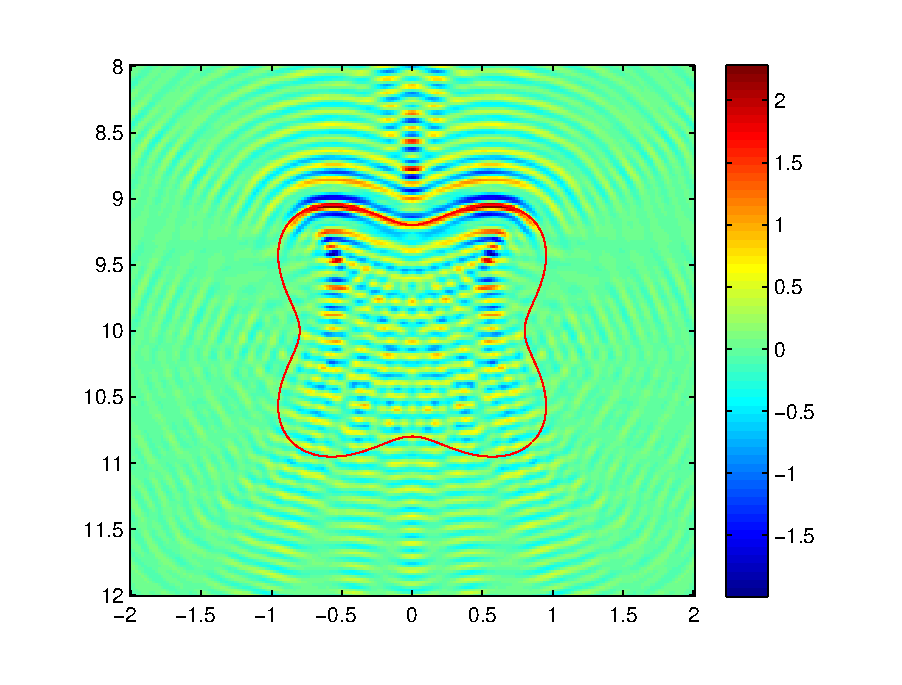
\includegraphics[width=0.32\textwidth]{./Img/graphic/p_leaf_5pi.eps}
	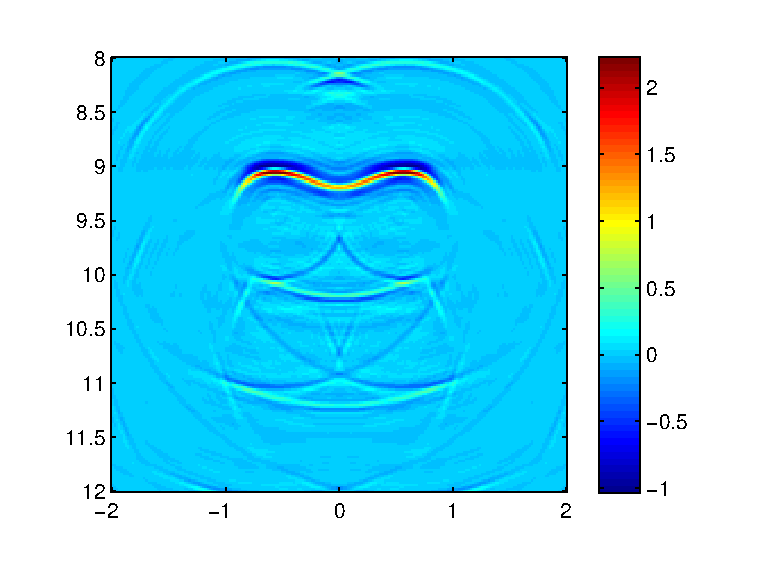
\includegraphics[width=0.32\textwidth]{./Img/graphic/p_leaf.eps}
	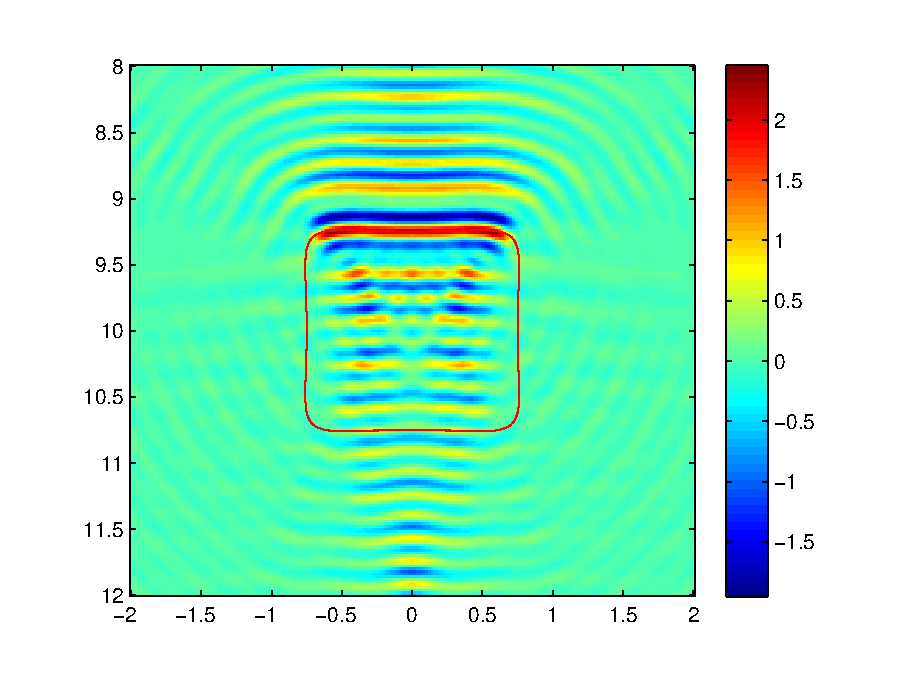
\includegraphics[width=0.32\textwidth]{./Img/graphic/rectangle_3pi.eps}
	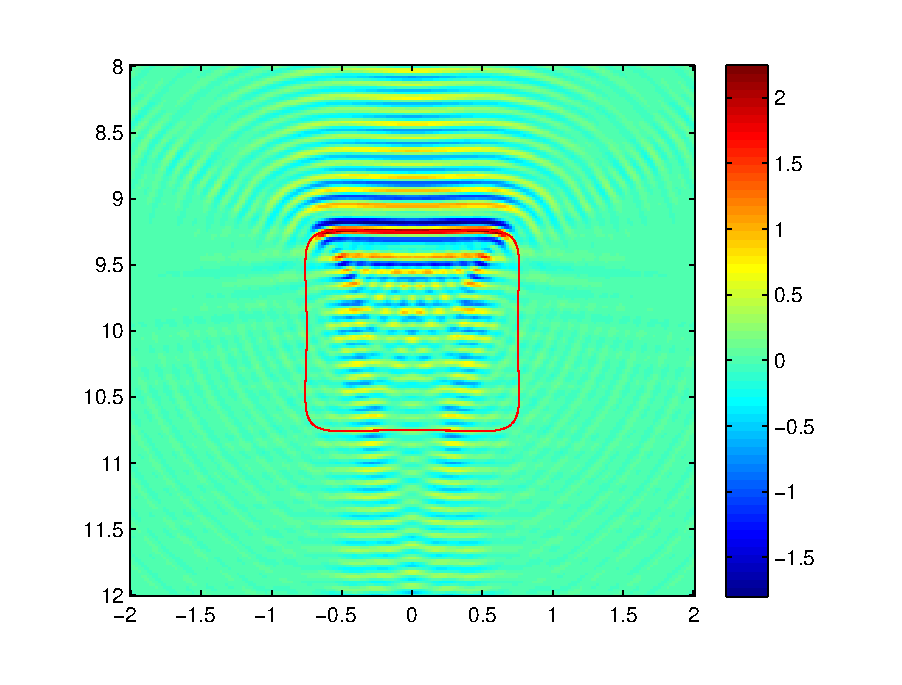
\includegraphics[width=0.32\textwidth]{./Img/graphic/rectangle_5pi.eps}
	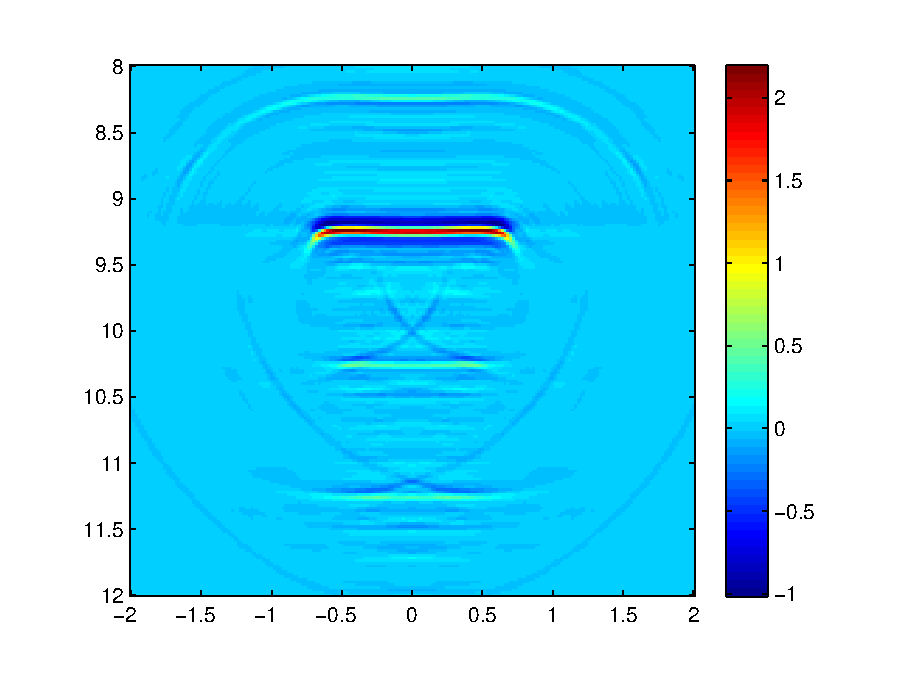
\includegraphics[width=0.32\textwidth]{./Img/graphic/rectangle.eps}
	
	\caption{算例 1: 从上到下是不同形状的 Dirichlet 障碍物,依次是圆形,花生形,四叶草形 以及旋转后的方形的成像结果。 其中,第一列是关于单频的, 其角频率为 $\om=3\pi$, 第二列是关于单频的, 其角频率为 $\om=5\pi$ 以及第三列是关于多频叠加的}\label{figure_21}
\end{figure}
如图 \ref{figure_21}, 针对不同形状的障碍物, RTM 算法都可以将其上沿给成像出来。 而且, 当对多个单频成像进行叠加后得到的多频成像结果可以显著提高单频的成像效果。

\bigskip
\textbf{算例 2}.
我们考虑针对 Dirichlet 障碍物,  Neumann 障碍物, 阻抗障碍物, 以及可穿透障碍物进行成像。 每个成像区域都为 $\Om=(-2,2) \times (8, 12)$ 且其样本点网格取为 $201 \times 201$。 我们设置发射器和接收器数量为 $N_s = N_r = 401$, 角频率为 $\om=2\pi$。 
\begin{figure}[htbp]
	\centering
	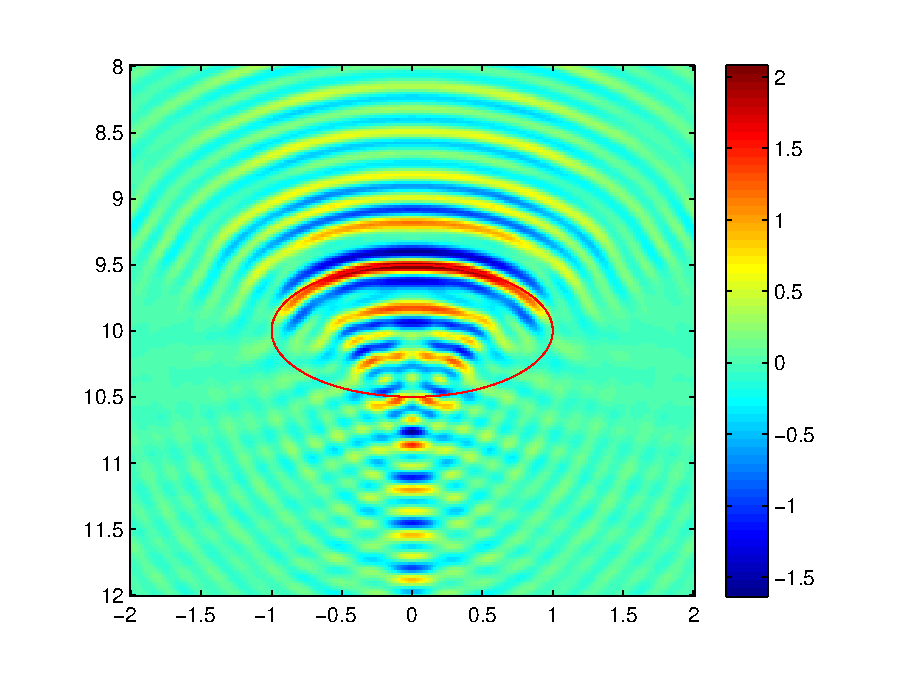
\includegraphics[width=0.24\textwidth]{./Img/graphic/circle_3pi.eps}
	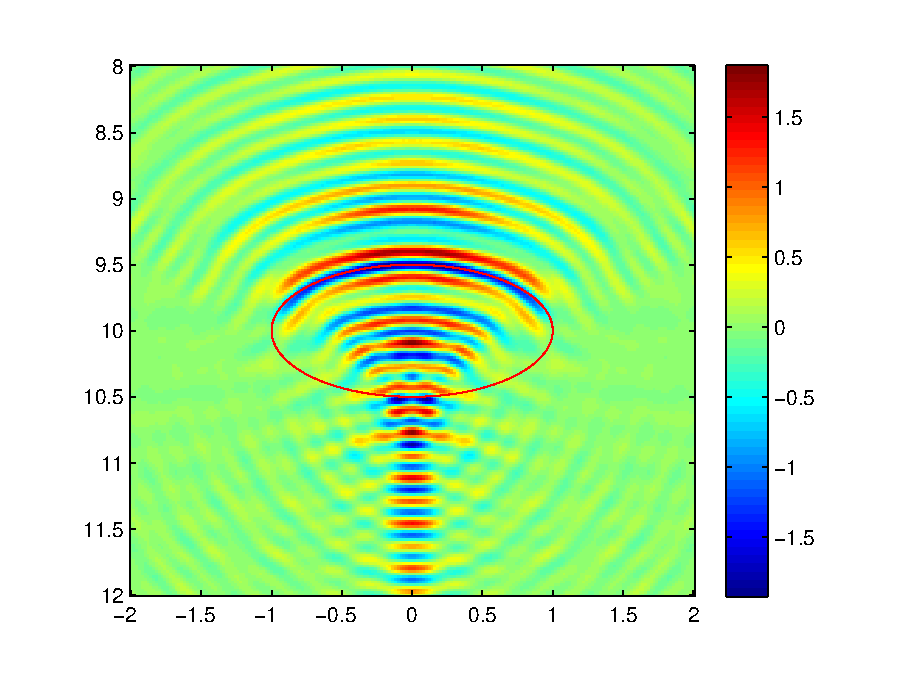
\includegraphics[width=0.24\textwidth]{./Img/graphic/circle_3pi_neumann.eps}
	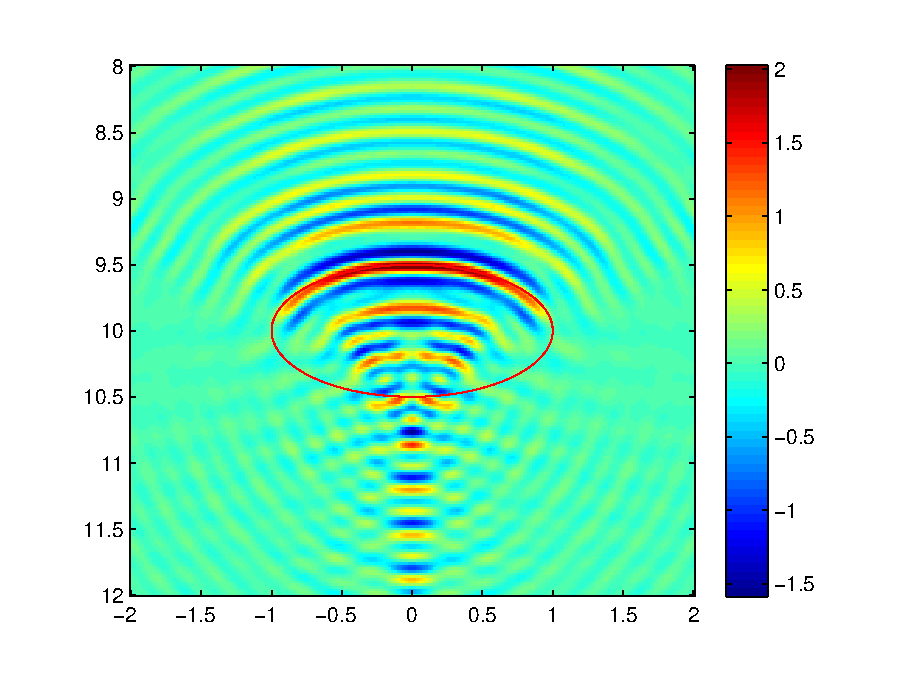
\includegraphics[width=0.24\textwidth]{./Img/graphic/circle_3pi_impedance_1.eps}
	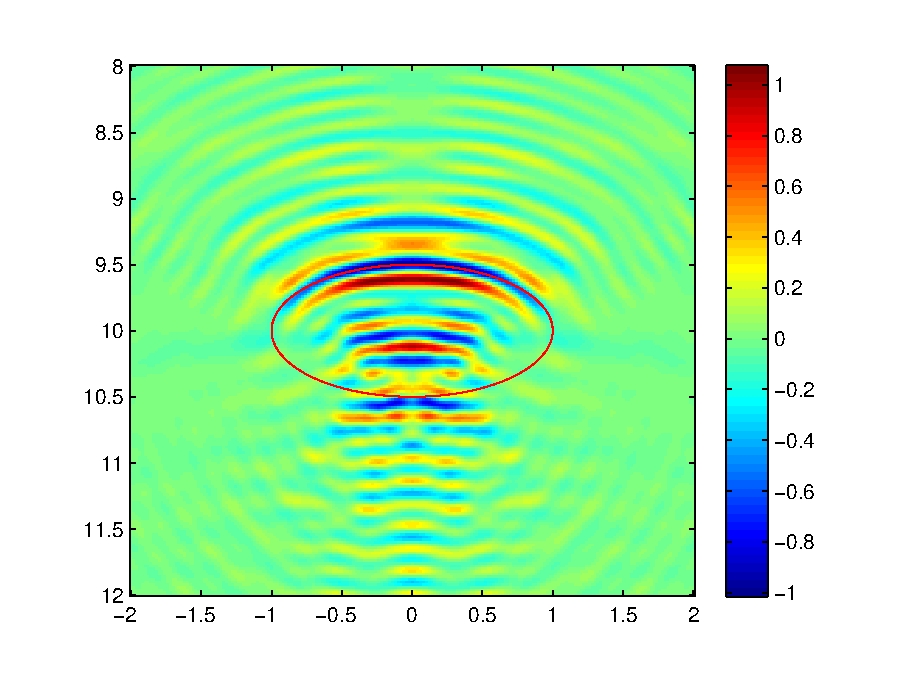
\includegraphics[width=0.24\textwidth]{./Img/graphic/circle_3pi_transmission.eps}
	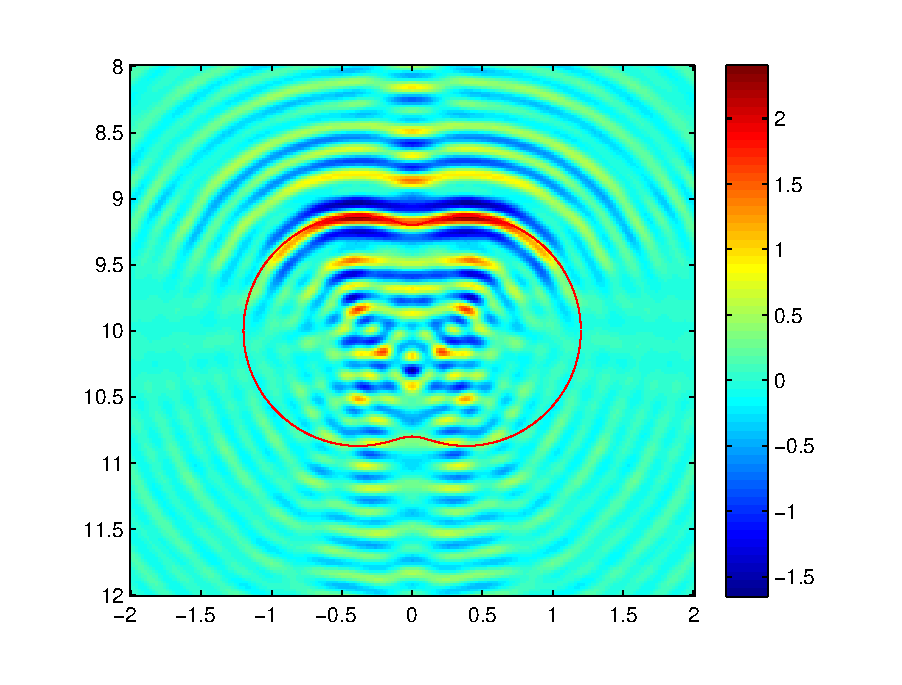
\includegraphics[width=0.24\textwidth]{./Img/graphic/peanut_3pi.eps}
	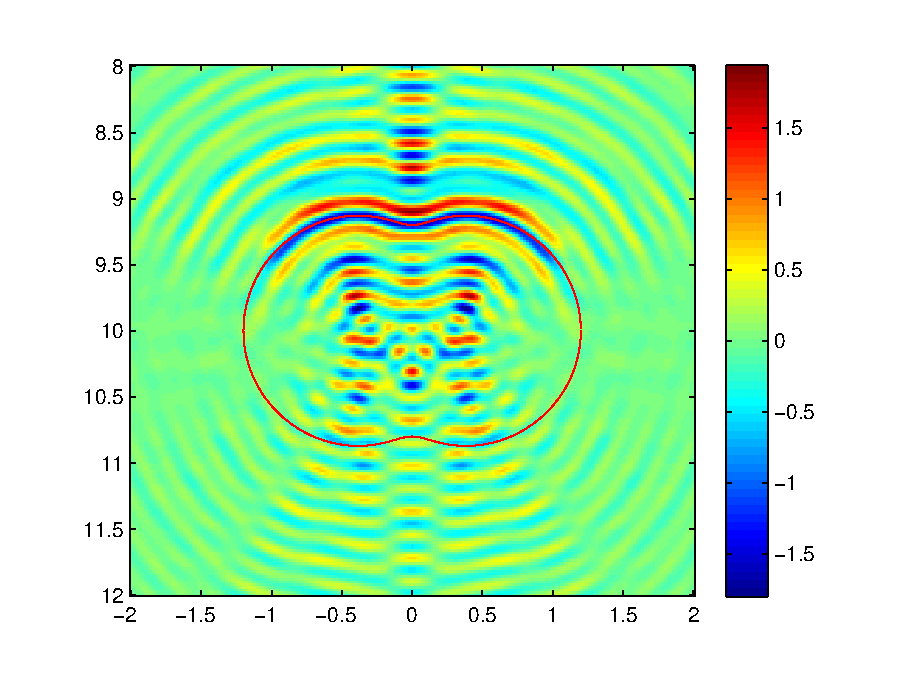
\includegraphics[width=0.24\textwidth]{./Img/graphic/peanut_3pi_neumann.eps}
	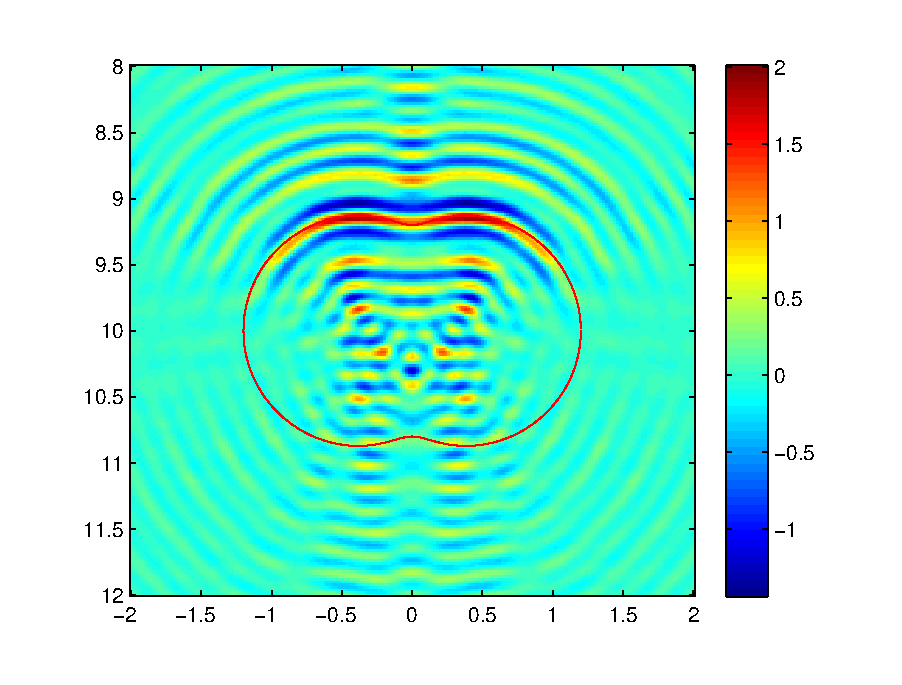
\includegraphics[width=0.24\textwidth]{./Img/graphic/peanut_3pi_impedance_1.eps}
	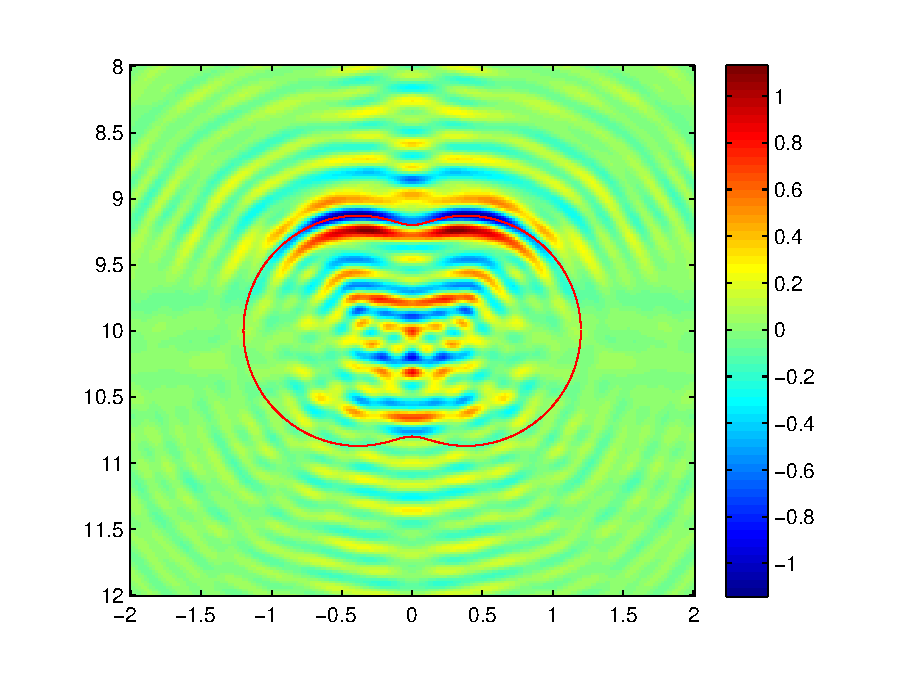
\includegraphics[width=0.24\textwidth]{./Img/graphic/peanut_3pi_transmission.eps}
	\caption{算例 2: 从左到右: Neumann 障碍物, 阻抗障碍物, 以及衍射指数为$n(x)=0.25$ 可穿透障碍物的成像结果 ; 第一行中的障碍物为圆形,第二行中的障碍物为花生。} \label{figure_11}
\end{figure}

成像结果见图 \ref{figure_11} 所示。我们可以清晰可见,对于不可穿透障碍物, 障碍物的上边界都被 RTM 方法成像出来,且这部分边界刚好是正对着分布着发射器和接收器的半空间表面 $\Ga_0$,相比较下, 位于障碍物边界的阴暗部分的点以及远离边界的点的成像函数值都是非常小的。

显然, 成像算法(\ref{cor})与障碍是否可穿透, 可穿透时是哪种边界条件无关。在不知道障碍物边界的先验信息下,如图\ref{figure_11}所示,针对不同类型的障碍物, RTM 方法都可以成像。

\bigskip
\textbf{算例 3} 我们考虑来针对两个障碍物同时成像。第一个模型是在水平方向上并排两个障碍物; 第二个模型是一个圆和一个花生在竖直方向上排列 (圆上花生下);第三个模型是一个圆和一个花生在竖直方向上排列 (圆下花生上)。 针对单频的成像实验, 我们取角频率为 $\om=3\pi$ , 而针对多频的成像实验, 我们取多频角频率为 $\om=\pi\times[2:0.5:8]$ 。 如图 \ref{figure_31} 所示,是第一个模型的成像结果。 其成像区域为 $\Om=(-4, 4) \times (8,12)$ , 采样网格点数量 $401 \times 201$。我们设置发射器和接收器数量为 $N_s = N_r = 301$。 如图 \ref{figure_32}和\ref{figure_33} 所示,是第二个模型和第三个模型的成像结果。 其成像区域为 $\Om=(-4, 4)\times (8,12)$ , 采样网格点数量 $401 \times 401$。 我们设置发射器和接收器数量为 $N_s = N_r = 301$。在图 \ref{figure_31} ,图 \ref{figure_32}和图\ref{figure_33} 中的多频 RTM 成像只是简单地将每个不同的单频 RTM 成像结果直接叠加而得。 我们可以发现, 通过这样简单的多个单频叠加后, 成像质量得到显著地提高。
 
\begin{figure}[htbp]
	\centering
	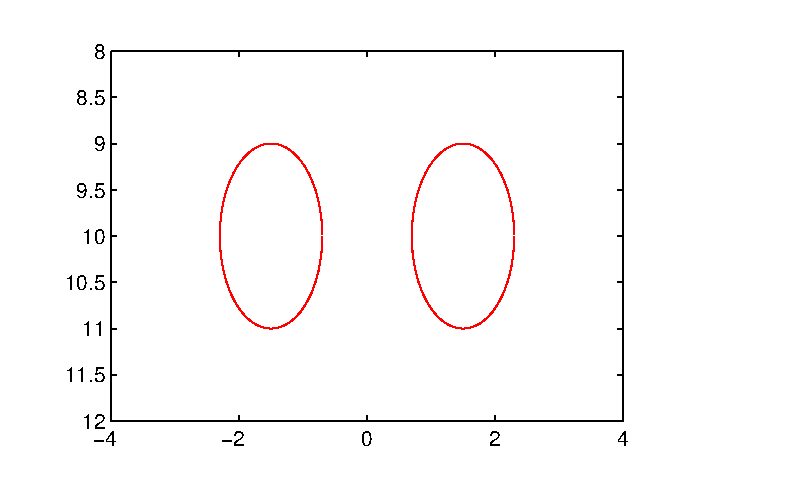
\includegraphics[width=0.32\textwidth,height=0.16\textheight]{./Img/graphic/bi_circle_profile.eps}
	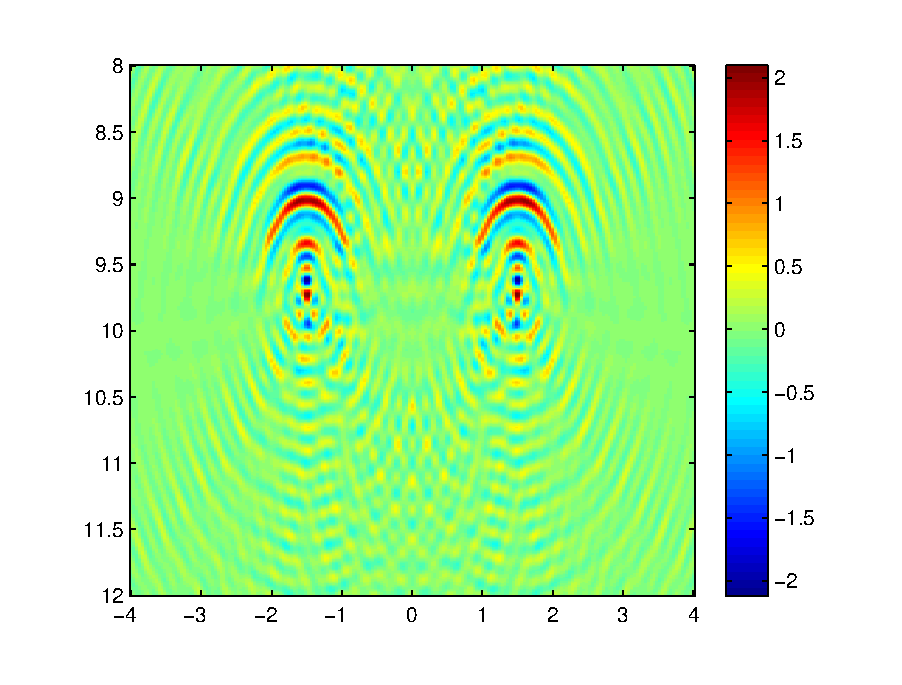
\includegraphics[width=0.32\textwidth]{./Img/graphic/bi_circle_3pi.eps}
	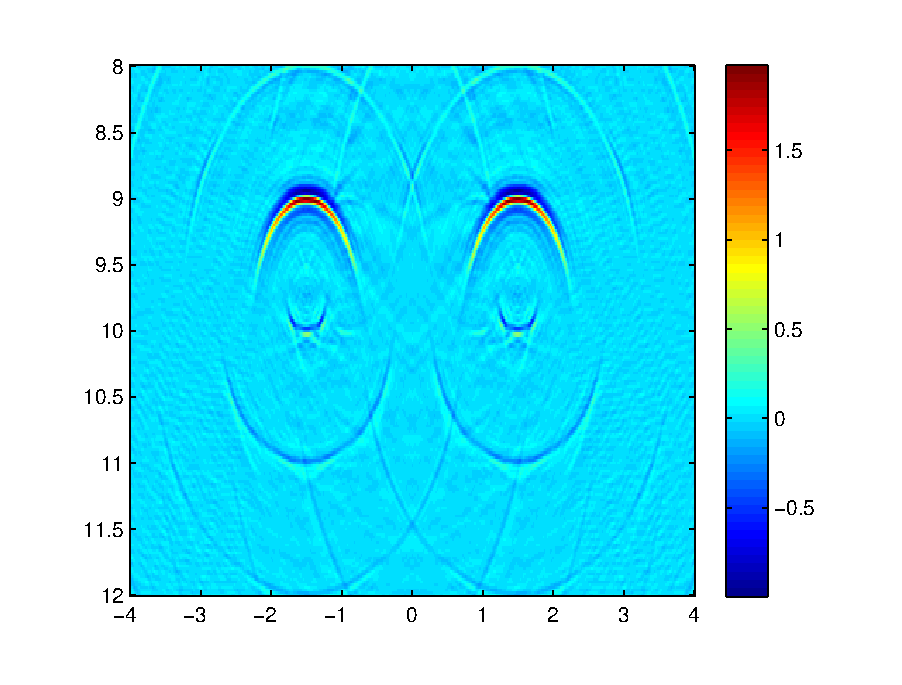
\includegraphics[width=0.32\textwidth]{./Img/graphic/bi_circle.eps}
	
	\caption{算例 3: 从左到右分别为,  真实的两个障碍物:圆, 关于单频角频率为 $\om=3\pi$的成像结果, 关于多频叠加的成像结果。}\label{figure_31}
\end{figure}

\begin{figure}[htbp]
	\centering
	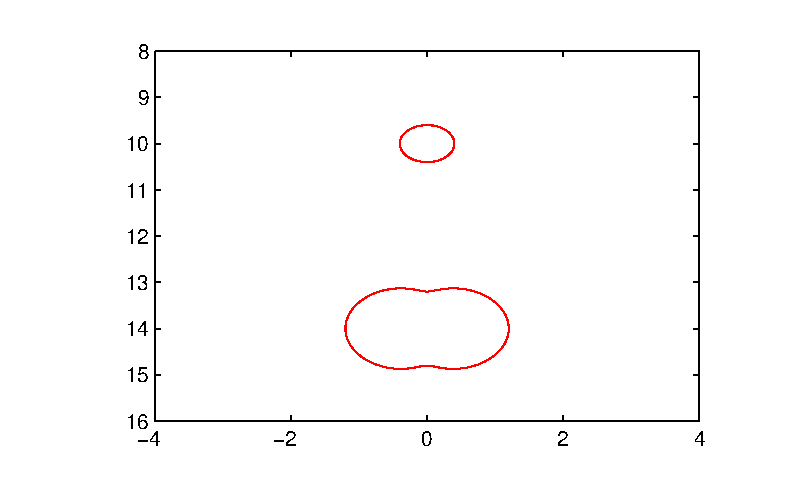
\includegraphics[width=0.32\textwidth,height=0.16\textheight]{./Img/graphic/circle_0_4_peanut_1_profile.eps}
	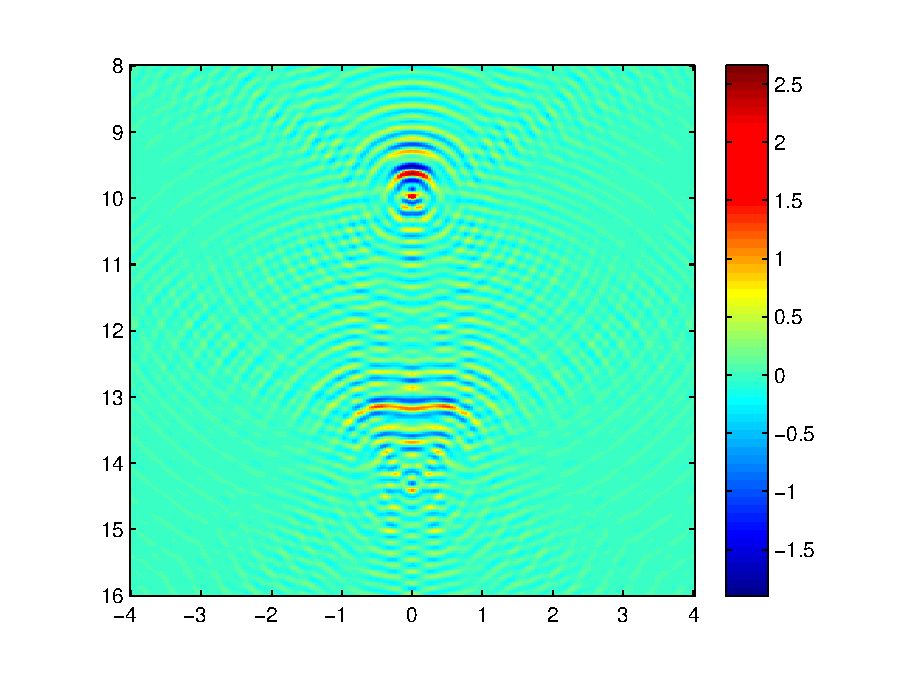
\includegraphics[width=0.32\textwidth]{./Img/graphic/circle_0_4_peanut_1_3pi_1.eps}
	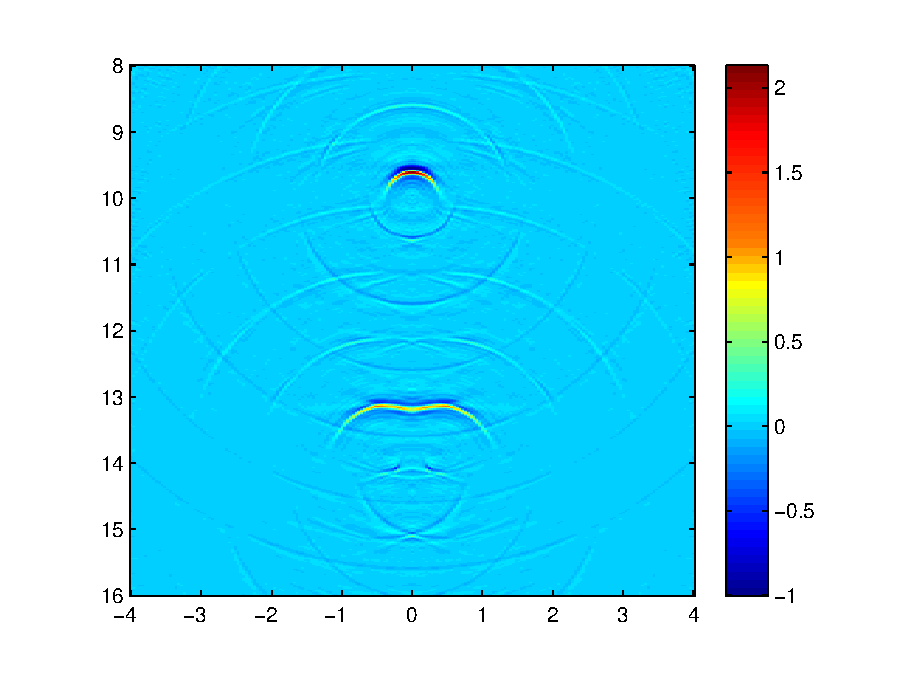
\includegraphics[width=0.32\textwidth]{./Img/graphic/circle_0_4_peanut_1_multi_1.eps}
	
	\caption{算例 3: 从左到右分别为,  真实的两个障碍物:圆上和花生下, 关于单频角频率为 $\om=3\pi$的成像结果, 关于多频叠加的成像结果。}\label{figure_32}
\end{figure}


\begin{figure}[htbp]
 	\centering
 	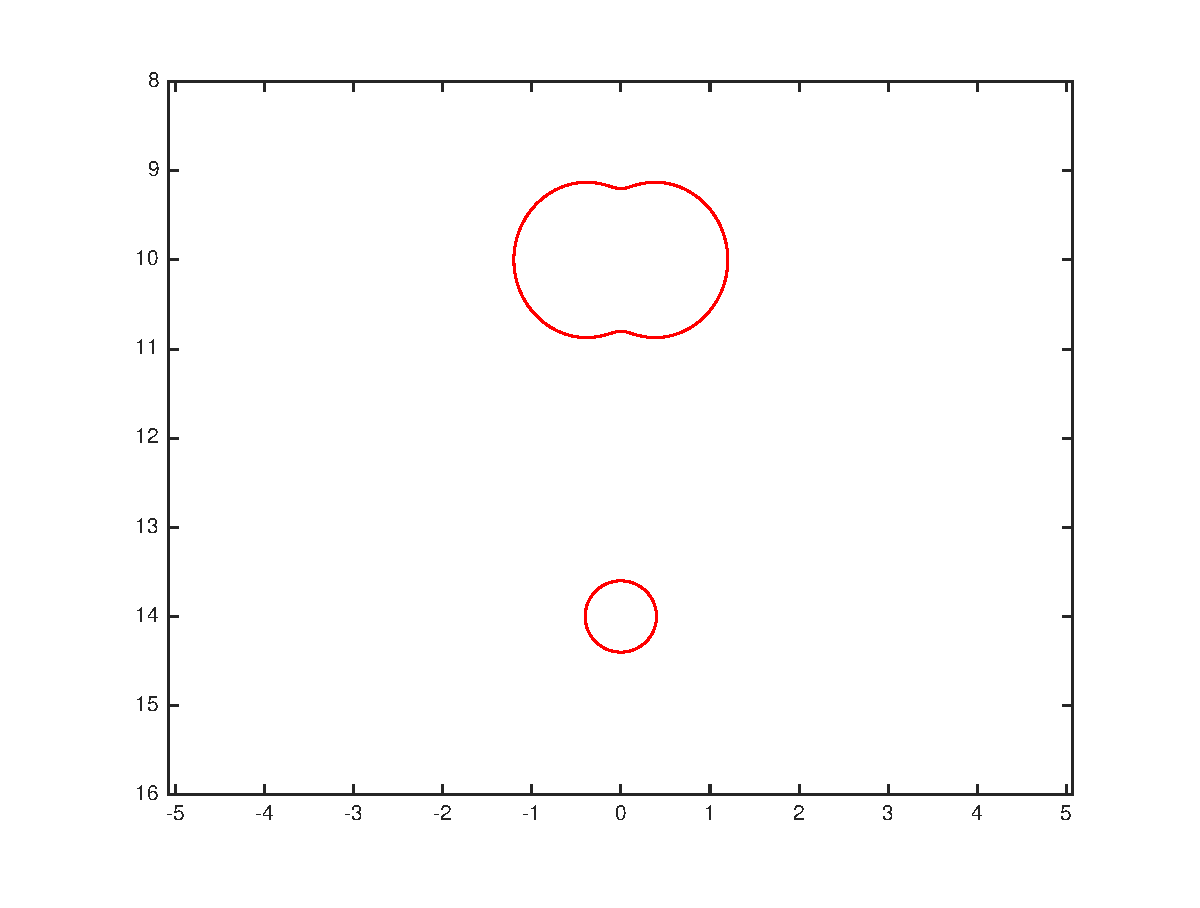
\includegraphics[width=0.32\textwidth,height=0.16\textheight]{./Img/graphic/circle_0_4_peanut_1_profile_reverse.eps}
 	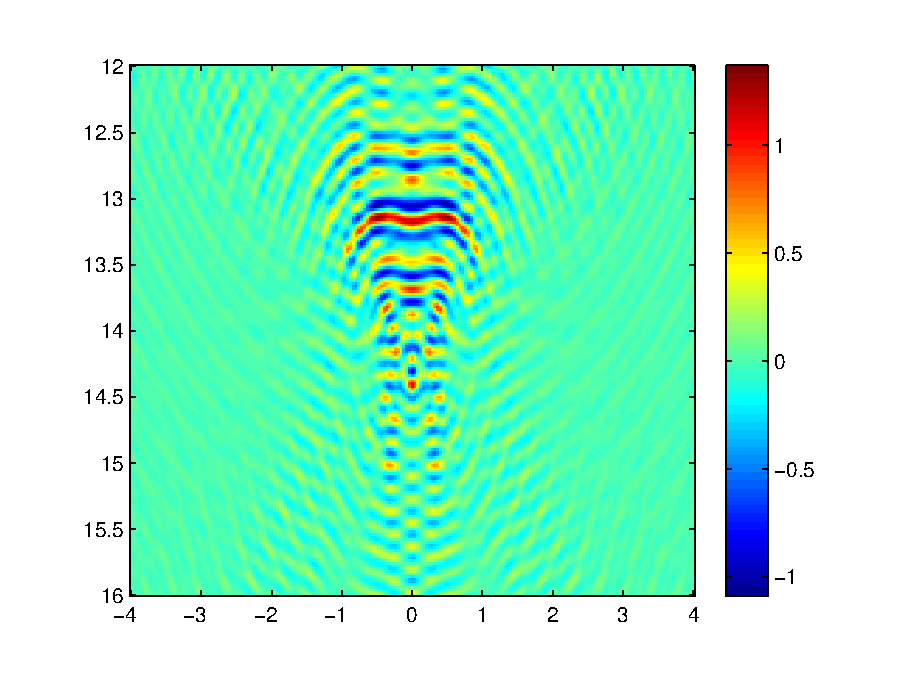
\includegraphics[width=0.32\textwidth]{./Img/graphic/circle_0_4_peanut_1_3pi_down.eps}
 	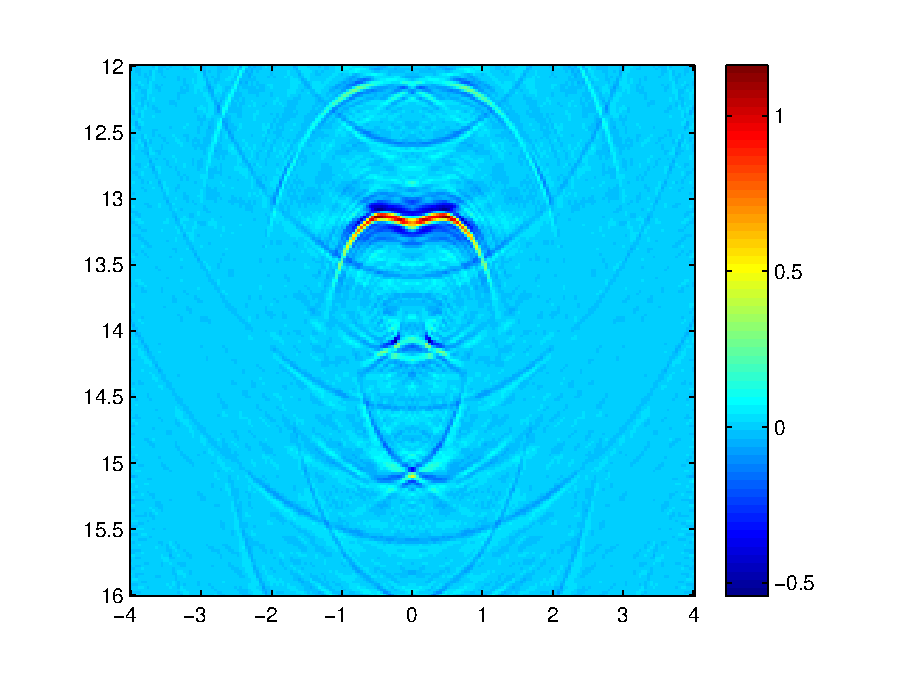
\includegraphics[width=0.32\textwidth]{./Img/graphic/circle_0_4_peanut_1_multi_down.eps}
 	
 	\caption{算例 3: 从左到右分别为,  真实的两个障碍物:圆下和花生上, 关于单频角频率为 $\om=3\pi$的成像结果, 关于多频叠加的成像结果。}\label{figure_33}
 \end{figure}

  如图 \ref{figure_32} 所示, 我们发现即使圆形挡在花生的上面, RTM 算法还是可以将圆和花生的上沿都给成像出来, 进一步说明了 RTM 算法的有效性。而如图 \ref{figure_33} 所示,我们法向当大一号的花生挡在圆的上面时,只能将花生的上沿给成像出来, 而无法对圆成像,我们可以猜测在这种情况下由于花生的阻挡,可能在 $\Ga_0$ 上接受到关于圆的信息是极少的。
  
\bigskip
\textbf{算例 4}
我们考虑半空间弹性波 RTM 算法关于复加性 Gaussian 噪声的稳定性。 这里加性 Gaussian 噪声定义为 
\ben
u_{\rm noise}=u_s+\nu_{\rm noise},
\een
其中 $u_s$ 合成的散射数据, $\nu_{\rm noise}$ 是 Gaussian 噪声, 且均值为0, 其标准差是散射数据 $|u_s|$ 中最大值的 $\sigma$ 倍, 即为 $\nu_{\rm noise}=\frac{\sigma \max |u_s|}{\sqrt{2}}(\ep_1+\i\ep_2)$ 和 $\ep_i\thicksim \mathcal{N}(0,1)$。

\begin{figure}[htbp]
	\centering
	\includegraphics[width=0.32\textwidth]{./Img/graphic/bi_circle_4pi_error2.eps}
	\includegraphics[width=0.32\textwidth]{./Img/graphic/bi_circle_4pi_error4.eps}
	\includegraphics[width=0.32\textwidth]{./Img/graphic/bi_circle_4pi_error6.eps}
	\includegraphics[width=0.32\textwidth]{./Img/graphic/bi_circle_multi_2_8_error2.eps}
	\includegraphics[width=0.32\textwidth]{./Img/graphic/bi_circle_multi_2_8_error4.eps}
	\includegraphics[width=0.32\textwidth]{./Img/graphic/bi_circle_multi_2_8_error6.eps}
	
	\caption{算例 4: 从左到右,分别是含有噪声水平 $\mu =  0.2; 0.3; 0.4$ Dirichlet 障碍物的成像结果。 其中第一行是关于单频成像, 其角频率为 $\om=4\pi$, 第二行是多个单频成像的叠加}\label{figure_4}
\end{figure}

如图 \ref{figure_4} 所示, 即使在加了加性 Gaussian 噪声后, 单频 RTM 成像算法还是可以把障碍物的上沿给清晰成像,说明了该算法的稳定性。  而且在通过多个角频率 $\omega = \pi\times [2:0.5:8]$ 的成像结果叠加后, 其成像质量显著提高,而且消除了 Gaussian 噪声的影响。

从上述数值结果, 我们可以看出,利用同一个成像函数,在不需要障碍的任何先验信息下,都能够对障碍物的上边界做到有效成像。由于,散射体嵌入在一个半空间中,发射面和接受面都在半空间表面, 所以无法对下边界成像也是符合物理意义的。

\section{本章小结}

本章基于逆时偏移的思想提出了针对半空间弹性波反散射障碍物问题的直接成像法。与地球物理领域中现行的做法不同是, 我们不再对反传波进行波场分离, 然后再与相应分离的入射波场做互相关。 这里我们直接利用反传的混合耦合波场与入射波做互相关。当背景介质是均匀各项同性时, 基于波场分解的逆时偏移算法也可以用本章类似的论证来得到分辨率分析。 然而, 当背景介质是非均匀时,Helmholtz 分解很难再将混合耦合波场精确分解。 此时, 本章讨论的直接成像法可以很容易的推广到非均匀背景介质情形, 甚至是各向异性的背景介质。

观察本章的数值成像函数 $\ref{cor}$, 这里只涉及到矩阵与向量的乘法,相比于线性采样法或是分解法, 该算法不需要求解积分方程。与迭代法相比, 该算法不需要知道障碍物的先验信息。因此, 本章提出的半空间反散射问题的逆时偏移算法是一种快速有效的数值重构算法。
